\chapter{椭圆曲线与模形式}\label{ch:5}

\begin{quote}\small\itshape
{\emergencystretch=3em Fermat 是有史以来最令人着迷的数学人物之一，是解析几何的创立者（与 Descartes 共同创立）、微积分的奠基人之一，以及无可争议的现代数论奠基人.\par}
\end{quote}
\vspace{-0.5em}
\hfill \small \cite{weil1973}.

我们希望理解 $\mathbb{Q}$ 上椭圆曲线 $E$ 的 $L$-函数 $L(E/\mathbb{Q}, s)$, 即希望理解数列
\[
N_2, N_3, N_5, \dots, N_p, \dots, \qquad N_p = \#E_p(\mathbb{F}_p),
\]
或等价地数列 $a_2, a_3, a_5, \dots, a_p, \dots$, 其中 $a_p = p + 1 - N_p$. 没有直接方法做到这一点. 相反, 我们将看到模曲线与模形式的研究如何导向那些可能是 $\mathbb{Q}$ 上椭圆曲线的 $L$-函数的函数, 然后看到 Wiles 等人如何证明 $\mathbb{Q}$ 上椭圆曲线的所有 $L$-函数确实来自模形式.

\section{\texorpdfstring{Riemann 曲面 $X_0(N)$}{Riemann 曲面 X0(N)}}\label{sec:5.1}

\subsection*{群作用\index{qunzuoyong@群作用(group action)}下的 Riemann 曲面商}

我们需要把 Riemann 曲面定义为其他更简单的 Riemann 曲面在群作用下的商. 这可以相当复杂. 下面的例子会有帮助.

\begin{example} \label{thm:5.1.1} 
令 $n\in\mathbb{Z}$ 按 $z\mapsto z + n$ 作用在 $\mathbb{C}$ 上. 拓扑上 $\mathbb{C}/\mathbb{Z}$ 是圆柱面. 记 $\pi\colon\mathbb{C}\to\mathbb{C}/\mathbb{Z}$ 为商映射. 则 $\mathbb{C}/\mathbb{Z}$ 有唯一的复结构使 $\pi$ 是 Riemann 曲面的局部同构. $\mathbb{C}/\mathbb{Z}$ 的开子集上的函数 $f\colon U\to\mathbb{C}$ 对此结构全纯 (分别地亚纯), 当且仅当 $f\circ\pi$ 全纯 (分别地亚纯). 故 $U\subset\mathbb{C}/\mathbb{Z}$ 上的全纯函数可等同于 $\pi^{-1}(U)$ 上在 $\mathbb{Z}$ 下不变 (即满足 $g(z+1) = g(z)$) 的全纯函数 $g$. 例如 $q(z) = e^{2\pi iz}$ 定义 $\mathbb{C}/\mathbb{Z}$ 上的全纯函数. 事实上它给出同构 $\mathbb{C}/\mathbb{Z}\to\mathbb{C}^{\times}$, 其逆 $\mathbb{C}^{\times}\to\mathbb{C}/\mathbb{Z}$ (由定义) 是 $(2\pi i)^{-1}\log$.
\end{example}

\begin{example} \label{thm:5.1.2} 
设 $D$ 为单位开圆盘 $\{z \mid |z| < 1\}$, $\Gamma$ 为作用在 $D$ 上并固定 $0$ 的有限群. Schwarz 引理 (\cite[III, 3]{cartan1963}) 表明 $D$ 的固定 $0$ 的自同构是映射 $z\mapsto\zeta z$, $|\zeta| = 1$, 故
\[
\operatorname{Aut}(D) = \{z\in\mathbb{C} \mid |z| = 1\}\cong\mathbb{R}/\mathbb{Z}.
\]
由此 $\Gamma$ 是有限循环群. 设 $z\mapsto\zeta z$ 生成之, 且 $\zeta$ 的阶为 $m$. 则 $z^m$ 在 $\Gamma$ 下不变, 故定义 $\Gamma\setminus D$ 上的函数, 它事实上是同胚 $\Gamma\setminus D\to D$, 从而定义 $\Gamma\setminus D$ 上的复结构.

设 $\pi\colon D\to\Gamma\setminus D$ 为商映射. 开集 $U\subset\Gamma\setminus D$ 上的全纯函数空间可等同于 $\pi^{-1}(U)$ 上满足 $g(\zeta z) = g(z)$ (对所有 $z$) 的全纯函数空间, 故形如 $g(z) = h(z^m)$ ($h$ 全纯). 注意若 $\pi(Q) = P = 0$, 则 $\operatorname{ord}_P(f) = \frac{1}{m}\operatorname{ord}_Q(f\circ\pi)$.
\end{example}

设 $\Gamma$ 为作用在 Riemann 曲面 $X$ 上的群. $\Gamma$ 的基本区域 (fundamental domain) 是 $X$ 的连通开子集 $D$ 满足:
\begin{enumerate}[label=\textup{(\alph*)}]
\item $D$ 中没有两个点在 $\Gamma$ 的同一轨道中;
\item $D$ 的闭包 $\bar{D}$ 含每个轨道至少一个元素.
\end{enumerate}
例如,
\[
D = \{z\in\mathbb{C} \mid 0 < \Re(z) < 1\}
\]
是 $\mathbb{Z}$ 如 \ref{thm:5.1.1} 作用在 $\mathbb{C}$ 上的基本区域, 而
\[
D_0 = \{z\in D \mid 0 < \arg z < 2\pi/m\}
\]
是 $\mathbb{Z}/m\mathbb{Z}$ 如 \ref{thm:5.1.2} 作用在单位圆盘上的基本区域.

\subsection*{Riemann 曲面 $X(\Gamma)$}

设 $\Gamma$ 为 $\SL_2(\mathbb{Z})$ 中有限指数的子群. 我们想在商 $\Gamma\setminus\mathbb{H}$ 上定义 Riemann 曲面结构. 可以做到, 但所得曲面不紧. 相反, 需形成商 $\Gamma\setminus\mathbb{H}^*$, 其中 $\mathbb{H}^*$ 真包含 $\mathbb{H}$.

\paragraph{$\SL_2(\mathbb{Z})$ 在上半平面上的作用 (The action of $\SL_2(\mathbb{Z})$ on the upper half-plane)}
回忆 (III, \S\ref{sec:3.1}) $\SL_2(\mathbb{Z})$ 按规则
\[
\begin{pmatrix}a & b\\ c & d\end{pmatrix}z = \frac{az+b}{cz+d}
\]
作用在 $\mathbb{H} = \{z \mid \Im(z) > 0\}$ 上. 注意 $-I$ 平凡作用, 故该作用穿过模群 (modular group)\index{moqun@模群(modular group)} $\PSL_2(\mathbb{Z}) \overset{\text{def}}{=} \SL_2(\mathbb{Z})/\{\pm I\}$.

令
\[
S = \begin{pmatrix}0 & -1\\ 1 & 0\end{pmatrix}, \quad z\mapsto Sz = -\frac{1}{z}
\]
(``反演对称''), 与
\[
T = \begin{pmatrix}1 & 1\\ 0 & 1\end{pmatrix}, \quad z\mapsto Tz = z + 1
\]
(平移). 在 $\PSL_2(\mathbb{Z})$ 中, $S^2 = 1$, $(ST)^3 = 1$.

\begin{proposition} \label{thm:5.1.3} 
设
\[
D = \left\{z\in\mathbb{H} \;\Big|\; |z| > 1, \ -\frac{1}{2} < \Re(z) < \frac{1}{2}\right\}.
\]
\begin{minipage}[t]{0.62\textwidth}
\begin{enumerate}[label=\textup{(\alph*)}]
\item $D$ 是 $\PSL_2(\mathbb{Z})$ 的基本区域; 且 $\bar{D}$ 中两个元素 $z\neq z'$ 在同一轨道当且仅当
\begin{enumerate}[label=\textup{(\roman*)}]
\item $\Re(z) = \pm\frac{1}{2}$ 且 $z' = z\mp 1$ (即 $z' = Tz$ 或 $z = Tz'$); 或
\item $|z| = 1$ 且 $z' = -1/z = Sz$.
\end{enumerate}
特别地, $z$ 与 $z'$ 位于 $\bar{D}$ 的边界中.

\end{enumerate}
\begin{enumerate}[label=\textup{(\alph*)}]\setcounter{enumi}{1}
\item 设 $z\in\bar{D}$. $z$ 在 $\PSL_2(\mathbb{Z})$ 中的稳定子是 $\{1\}$, 除以下三种情形:
\begin{enumerate}[label=\textup{(\roman*)}]
\item $z = i$, 稳定子 $\langle S\rangle$;
\item $z = \rho = e^{2\pi i/6}$, 稳定子 $\langle TS\rangle$;
\item $z = \rho^2 = e^{2\pi i/3}$, 稳定子 $\langle ST\rangle$.
\end{enumerate}
群 $\PSL_2(\mathbb{Z})$ 由 $S$ 与 $T$ 生成.
\end{enumerate}
\end{minipage}%
\hfill
\begin{minipage}[t]{0.35\textwidth}
  \[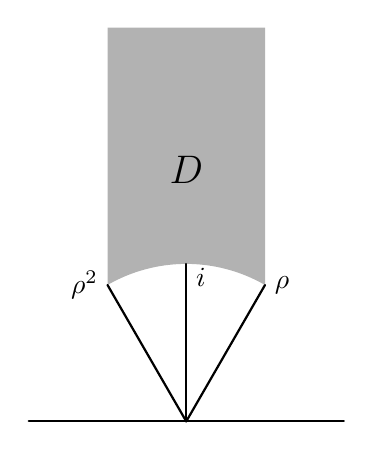
\begin{tikzpicture}[scale=2, line cap=round, line join=round]
        % 1. 定义基本参数
        % 这里的几何关系基于单位圆: rho = e^{i*pi/3}, rho^2 = e^{i*2pi/3}
        % 点的坐标: rho = (0.5, sqrt(3)/2), rho^2 = (-0.5, sqrt(3)/2)
        \def\sqthree{1.732/2} % sqrt(3)/2 约等于 0.866
        
        % 2. 绘制灰色阴影区域 D
        % 区域边界: 左垂直线 x=-0.5, 右垂直线 x=0.5, 下边界是单位圆弧
        \fill[gray!60] (-0.5, 2.5) -- (-0.5, \sqthree) 
            arc (120:60:1) -- (0.5, 2.5) -- cycle;

        % 3. 绘制辅助直线
        % 底部水平线 (实轴)
        \draw[thick] (-1, 0) -- (1, 0);
        
        % 从原点出发的三条射线
        \draw[thick] (0,0) -- (-0.5, \sqthree) coordinate (rho2);
        \draw[thick] (0,0) -- (0, 1) coordinate (i_point);
        \draw[thick] (0,0) -- (0.5, \sqthree) coordinate (rho);

        % 4. 绘制阴影区域的边界线（只画下方弧线, 两侧通常在示意图中由阴影界定）
        % 如果需要强化边界, 可以取消下面这行的注释: 
        % \draw[thick] (-0.5, 2.5) -- (-0.5, \sqthree) arc (120:60:1) -- (0.5, 2.5);

        % 5. 添加标签
        % D 标签在区域中心
        \node at (0, 1.6) {\Large $D$};
        
        % rho^2 标签（左侧）
        \node[left] at (rho2) {$\rho^2$};
        
        % rho 标签（右侧）
        \node[right] at (rho) {$\rho$};
        
        % i 标签（垂直线与圆弧交点处）
        % 原图中 i 放在交点右侧
        \node[below right, yshift=2pt] at (0, 1) {$i$};

    \end{tikzpicture}
    \]
\end{minipage}
\end{proposition}

\begin{proof}
定义 $G$ 为由 $S$ 和 $T$ 生成的 $\PSL_2(\mathbb{Z})$ 的子群 $\langle S, T \rangle$, 并设 $z \in \mathbb{H}$. 我们将证明存在一个 $g \in G$ 使得 $gz \in \bar{D}$. 若 $g = \begin{pmatrix} a & b \\ c & d \end{pmatrix} \in G$, 则
\[ \Im(gz) = \frac{\Im(z)}{|cz + d|^2} \]
对于任何 $N$, 满足 $|cz + d| < N$ 的整数对 $c, d \in \mathbb{Z}$ 只有有限多个, 因此可以选择 $g$ 使得 $|cz + d|$ 最小; 此时 $\Im(gz)$ 最大. 接下来我们选择 $n$ 使得
\[ -\frac{1}{2} \le \Re(T^n gz) \le \frac{1}{2}. \]
那么 $T^n gz \in \bar{D}$, 否则 $|T^n gz| < 1$, 并且
\[ \Im(ST^n gz) = \frac{\Im(T^n gz)}{|T^n gz|^2} > \Im(T^n gz) = \Im(gz), \]
这与 $g$ 的选择相矛盾. 我们已经证明了 $G \cdot \bar{D} = \mathbb{H}$; 特别地, $\PSL_2(\mathbb{Z}) \cdot \bar{D} = \mathbb{H}$. 

(b) 的证明以及 (a) 的其余部分是常规的 \cite[VII, 1.2]{serre1973}. 

对于 (c), 设 $h \in \PSL_2(\mathbb{Z})$, 并在 $D$ 中选择一个点 $z_0$. 存在 $G$ 中的元素 $g$ 使得 $ghz_0 \in \bar{D}$. 由于 $ghz_0$ 和 $z_0$ 处于同一个 $\PSL_2(\mathbb{Z})$ 轨道上, 根据 (a) 可知它们相等, 于是 (b) 表明 $gh = 1$. 因此 $h \in G$. 
\end{proof}

\begin{remark} \label{thm:5.1.4} 
\begin{enumerate}[label=\textup{(\alph*)}]
\item 可以证明模群 $\PSL_2(\mathbb{Z})$ 具有群展示(group presentation) $\langle S, T \mid S^2, (ST)^3 \rangle$. 换句话说, 它是 2 阶群 $\langle S \rangle$ 与 3 阶群 $\langle ST \rangle$ 的自由积. 许多有趣的有限群（例如, 除了四个之外的所有散在有限单群）都是由一个 2 阶元素和一个 3 阶元素生成的, 因此它们是 $\PSL_2(\mathbb{Z})$ 的商群. 
\item 设 $\Gamma$ 是 $\SL_2(\mathbb{Z})$ 的一个有限指数子群, 并记
\[ \SL_2(\mathbb{Z}) = \Gamma \gamma_1 \cup \dots \cup \Gamma \gamma_m \quad (\text{不交并}). \]
那么 $D' = \bigcup \gamma_i D$ 满足作为 $\Gamma$ 基本域的条件, 除了它可能不是连通的. 然而, 我们可以选取 $\gamma_i$ 使得 $D'$ 的闭包是连通的, 在这种情况下, 闭包的内部将成为 $\Gamma$ 的一个基本域. 
\end{enumerate}
\end{remark}

\subsection*{扩充上半平面}

$\SL_2(\mathbb{Z})$ 的元素通过射影线性变换作用于 $\mathbb{P}^1(\mathbb{C})$: 
\[ \begin{pmatrix} a & b \\ c & d \end{pmatrix} (z_1 : z_2) = (az_1 + bz_2 : cz_1 + \dd z_2). \]
我们将 $\mathbb{H}$、$\mathbb{Q}$ 和 $\{\infty\}$ 识别为 $\mathbb{P}^1(\mathbb{C})$ 的子集, 对应关系如下: 
\begin{align*}
    z &\leftrightarrow (z : 1) \quad z \in \mathbb{H} \\
    r &\leftrightarrow (r : 1) \quad r \in \mathbb{Q} \\
    \infty &\leftrightarrow (1 : 0).
\end{align*}

$\SL_2(\mathbb{Z})$ 在 $\mathbb{P}^1(\mathbb{C})$ 上的作用稳定了 $\mathbb{H}^* \stackrel{\text{def}}{=} \mathbb{H} \cup \mathbb{Q} \cup \{\infty\}$. 事实上: 
\begin{itemize}
    \item 若 $z \in \mathbb{H}$, 则 $\begin{pmatrix} a & b \\ c & d \end{pmatrix} (z : 1) = (az + b : cz + d) = \left( \frac{az+b}{cz+d} : 1 \right)$, 
    \item 若 $r \in \mathbb{Q}$, 则 $\begin{pmatrix} a & b \\ c & d \end{pmatrix} (r : 1) = (ar + b : cr + d) = 
    \begin{cases} 
        \left( \frac{ar+b}{cr+d} : 1 \right) & r \neq -\frac{d}{c} \\
        \infty & r = -\frac{d}{c},
    \end{cases}$
    \item $\begin{pmatrix} a & b \\ c & d \end{pmatrix} \infty = (a : c) = 
    \begin{cases} 
        \left( \frac{a}{c} : 1 \right) & c \neq 0 \\
        \infty & c = 0.
    \end{cases}$
\end{itemize}

在从 $\mathbb{H}$ 转换到 $\mathbb{H}^*$ 的过程中, 我们增加了一个额外的 $\SL_2(\mathbb{Z})$ 轨道. $\mathbb{H}^*$ 中不在 $\mathbb{H}$ 内的点被称为\emph{尖点 (cusps)}. 

\subsection*{$\mathbb{H}^*$ 上的拓扑}

我们按照以下方式赋予 $\mathbb{H}^*$ 拓扑: $\mathbb{H}$ 上的拓扑继承自 $\mathbb{C}$; 
集合
\[ \{z \mid \Im(z) > M\}, \quad M > 0 \]
构成了 $\infty$ 的一个基本邻域系; 集合
\[ \{z \mid |z - (a + ir)| < r\} \cup \{a\} \]
构成了 $a \in \mathbb{Q}$ 的一个基本邻域系. 可以证明 $\mathbb{H}^*$ 是Hausdorff空间, 且 $\SL_2(\mathbb{Z})$ 的作用是连续的. 

% TikZ 图表
\begin{center}
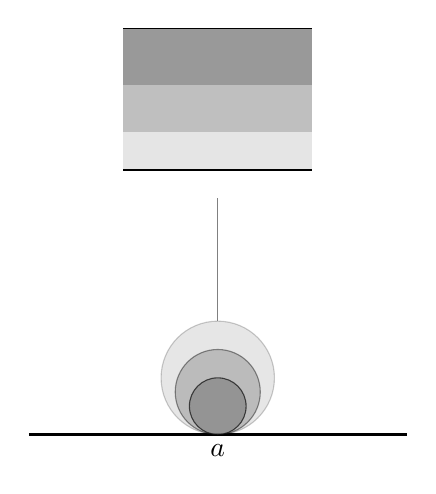
\begin{tikzpicture}[scale=1.2]
    % 绘制实轴
    \draw[thick] (-2,0) -- (2,0);
    \node[below] at (0,0) {$a$};

    % 绘制 a 处的邻域（圆/Horoballs）
    \foreach \r in {0.6, 0.45, 0.3} {
        \filldraw[fill=gray, opacity={1.1-\r*1.5}] (0,\r) circle (\r);
    }

    % 垂直连接线
    \draw[thin, gray] (0, 1.2) -- (0, 2.5);

    % 绘制无穷远处的邻域（水平带）
    \fill[gray!80] (-1, 3.7) rectangle (1, 4.3);
    \fill[gray!50] (-1, 3.2) rectangle (1, 3.7);
    \fill[gray!20] (-1, 2.8) rectangle (1, 3.2);
    \draw (-1, 2.8) -- (1, 2.8);
    \draw (-1, 4.3) -- (1, 4.3);

\end{tikzpicture}
\end{center}

\subsection*{$\Gamma \backslash \mathbb{H}^*$ 上的拓扑}

回想一下, 如果 $\pi: X \to Y$ 是一个满射且 $X$ 是拓扑空间, 那么 $Y$ 上的商拓扑定义为: 集合 $U$ 是开集当且仅当 $\pi^{-1}(U)$ 是开集. 通常情况下, 豪斯多夫空间在群作用下的商空间不一定是豪斯多夫空间, 即使轨道是闭的——这需要不同的轨道具有不交的开邻域. 

设 $\Gamma$ 是 $\SL_2(\mathbb{Z})$ 的有限指数子群. 离散群 $\Gamma$ 连续作用于 $\mathbb{H}$, 并且可以证明该作用是固有的\footnote{因此, 可以说 $\Gamma$ 在 $\mathbb{H}$ 上连续且固有地作用. 但在文献中, 通常称 $\Gamma$ 作用是“固有不连续的 (properly discontinuously)”. 参见 Lee 2003, p. 225 关于此术语的讨论. }. 即, 对于 $\mathbb{H}$ 中的任意一对点 $x, y$, 存在 $x$ 的邻域 $U$ 和 $y$ 的邻域 $V$ 使得集合
\[ \{ \gamma \in \Gamma \mid \gamma U \cap V \neq \emptyset \} \]
是有限的. 特别地, 这意味着 $\mathbb{H}$ 中每个点的稳定子群 (stabilizer) 都是有限的（这点我们已经知道了）. 


\begin{proposition} \label{thm:5.1.5}
\begin{enumerate}[label=\textup{(\alph*)}]
\item 对 $\mathbb{H}$ 的所有紧集 $A$ 与 $B$, $\{\gamma\in\Gamma \mid \gamma A\cap B\neq\varnothing\}$ 有限.
\item 每个 $z\in\mathbb{H}$ 有邻域 $U$ 使对 $\gamma\in\Gamma$, $\gamma U$ 与 $U$ 不相交, 除非 $\gamma z = z$.
\item 对 $\mathbb{H}$ 中不在同一 $\Gamma$-轨道中的点 $x, y$, 存在 $x$ 的邻域 $U$ 与 $y$ 的邻域 $V$ 使对所有 $\gamma\in\Gamma$ 有 $\gamma U\cap V = \varnothing$.
\end{enumerate}
\end{proposition}

\begin{proof}
\begin{enumerate}[label=\textup{(\alph*)}]
\item 由 $\Gamma$ 连续且真作用容易推出.

\item 设 $V$ 为 $z$ 的紧邻域, $S$ 为使 $V\cap\gamma V\neq\varnothing$ 但 $\gamma$ 不固定 $z$ 的 $\gamma\in\Gamma$ 的集合. 由 (a), $S$ 有限. 对每个 $\gamma\in S$, 选取 $z$ 的邻域 $V_\gamma$ 与 $\gamma z$ 的邻域 $W_\gamma$ 不相交, 令
\[
U = V\cap\bigcap_{\gamma\in S}(V_\gamma\cap\gamma^{-1}W_\gamma).
\]
对 $\gamma\in S$, $\gamma U\subset W_\gamma$. 因 $W_\gamma$ 与 $V_\gamma$ 不相交且 $V_\gamma$ 含 $U$, 这蕴含 $\gamma U$ 与 $U$ 不相交.

\item 选取 $x$ 的紧邻域 $A$ 与 $y$ 的紧邻域 $B$, 令 $S$ 为使 $\gamma A\cap B\neq\varnothing$ 的 (有限) $\gamma$ 集. 因 $\gamma x\neq y$, 对每个 $\gamma\in S$ 存在 $\gamma x$ 与 $y$ 的不相交邻域 $U_\gamma$ 与 $V_\gamma$. 则 $U = A\cap\bigcap_{\gamma\in S}\gamma^{-1}U_\gamma$ 与 $V = B\cap\bigcap_{\gamma\in S}V_\gamma$ 分别是 $x$ 与 $y$ 的邻域, 使对所有 $\gamma\in\Gamma$, $\gamma U$ 与 $V$ 不相交.
\end{enumerate}
\end{proof}

\begin{corollary} \label{thm:5.1.6}
空间 $\Gamma\setminus\mathbb{H}$ 是 Hausdorff 的.
\end{corollary}

\begin{proof}
设 $x$ 与 $y$ 是 $\mathbb{H}$ 中不在同一 $\Gamma$-轨道中的点, 按上一命题的 (c) 选取 $x$ 与 $y$ 的邻域 $U$ 与 $V$. 则 $\Gamma U$ 与 $\Gamma V$ 是 $\Gamma x$ 与 $\Gamma y$ 的不相交邻域.
\end{proof}

\begin{proposition} \label{thm:5.1.7}
空间 $\Gamma\setminus\mathbb{H}^*$ 是 Hausdorff 的且紧致.
\end{proposition}

\begin{proof}
由推论 \ref{thm:5.1.6}, 为证 $\Gamma\setminus\mathbb{H}^*$ Hausdorff, 只剩检验尖点附近, 留给读者 (见下一小节). 空间 $\Gamma\setminus\mathbb{H}^*$ 是 $\SL_2(\mathbb{Z})\setminus\mathbb{H}^*$ 的商, 后者紧致, 因 $\bar{D}\cup\{\infty\}$ 紧致.
\end{proof}

\subsection*{$\Gamma_0(N)\setminus\mathbb{H}^*$ 上的复结构}

我们将特别感兴趣的 $\SL_2(\mathbb{Z})$ 的子群是 Hecke 子群\index{Hecke@Hecke 子群(Hecke subgroups)}
\[
\Gamma_0(N) = \left\{\begin{pmatrix}a & b\\ c & d\end{pmatrix}\;\Big|\; c\equiv 0\pmod{N}\right\}.
\]
记 $\Gamma_0(1) = \SL_2(\mathbb{Z})$. 整数 $N$ 称为 $\Gamma_0(N)$ 的级 (level)\index{ji@级(level)}.

现在定义 $\Gamma_0(N)\setminus\mathbb{H}^*$ 上的复结构. 对 $z_0\in\mathbb{H}$, 选取 $z_0$ 的邻域 $V$ 使
\[
\gamma V\cap V\neq\varnothing\Rightarrow\gamma z_0 = z_0,
\]
令 $U = \pi(V)$——它开, 因 $\pi^{-1}U = \bigcup\gamma V$ 开.

若 $z_0$ 在 $\Gamma_0(N)$ 中的稳定子是 $\pm I$, 则 $\pi\colon V\to U$ 是同胚, 以 $\varphi$ 记其逆, 要求 $(U, \varphi)$ 是坐标邻域.

若 $z_0$ 在 $\Gamma_0(N)$ 中的稳定子 $\neq\{\pm I\}$, 则它是 $2m$ 阶循环群且 $m = 2$ 或 $3$ (它在 $\Gamma_0(N)/\{\pm I\}$ 中的像阶为 $2$ 或 $3$)——见 \ref{thm:5.1.3}b. 分式线性变换
\[
\lambda\colon\mathbb{H}\to D, \quad z\mapsto\frac{z - z_0}{z - \bar{z}_0},
\]
把 $z_0$ 送到单位圆盘 $D$ 中的 $0$. 存在良定义的映射 $\varphi\colon U\to\mathbb{C}$ 使 $\varphi(\pi(z)) = \lambda(z)^m$, 要求 $(U, \varphi)$ 是坐标邻域 (参看例 \ref{thm:5.1.2}).

再考虑 $z_0 = \infty$. 选取 $V$ 为 $\infty$ 的邻域 $\{z\mid \Im(z) > 2\}$, 令 $U = \pi(V)$. 若
\[
z\in V\cap\gamma V, \quad \gamma = \begin{pmatrix}a & b\\ c & d\end{pmatrix}\in\Gamma_0(N),
\]
则
\[
2\le\Im(\gamma z) = \frac{\Im(z)}{|cz + d|^2}\le\frac{1}{|c|^2\Im(z)}\le\frac{1}{2|c|^2}
\]
故 $c = 0$. 因此
\[
\gamma = \pm\begin{pmatrix}1 & m\\ 0 & 1\end{pmatrix},
\]
故存在良定义的映射 $\varphi\colon U\to\mathbb{C}$ 使 $\varphi(\pi(z)) = e^{2\pi iz}$, 要求 $(U, \varphi)$ 是坐标邻域 (参看例 \ref{thm:5.1.1}).

对 $z_0\in\mathbb{Q}$, 选取 $\beta\in\SL_2(\mathbb{Z})$ 使 $\beta(z_0) = \infty$, 类似处理.

\begin{proposition} \label{thm:5.1.8}
上面定义的坐标邻域相容, 故在 $\Gamma_0(N)\setminus\mathbb{H}^*$ 上定义 Riemann 曲面结构.
\end{proposition}

\begin{proof}
常规练习.
\end{proof}

把 Riemann 曲面 $\Gamma_0(N)\setminus\mathbb{H}^*$ 记为 $X_0(N)$, 其开子曲面 $\Gamma_0(N)\setminus\mathbb{H}$ 记为 $Y_0(N)$.

\subsection*{$X_0(N)$ 的亏格}

Riemann 曲面的亏格可通过``三角剖分''并使用公式
\[
2 - 2g = V - E + F
\]
计算, 其中 $V$ 是顶点数, $E$ 是边数, $F$ 是面数. 例如, 球面可从正四面体投影出去来三角剖分, 此时 $V = 4$, $E = 6$, $F = 4$, 故如愿 $g = 0$.

\begin{proposition} \label{thm:5.1.9}
Riemann 曲面 $X_0(1)$ 亏格为零.
\end{proposition}

\begin{proof}
取赤道上三点及上下半球为面, 得球面的一个``假''三角剖分, 它给出正确的亏格 $2 = 3 - 3 + 2$, 但违反三角剖分的通常定义 (要求任两个三角形交于单边、单点或不交). 加上北极点为顶点并与赤道三顶点相连, 可变成合法三角剖分.

取三个顶点 $\rho$, $i$ 与 $\infty$ 及连接它们的显然曲线 ($D$ 的边界上两条及从 $i$ 到 $\infty$ 的虚轴一条), 得 $X_0(1)$ 的一个假三角剖分. 在 $D$ 中实部 $> 0$ 处加上第四点并与 $\rho$, $i$, $\infty$ 相连, 可变成合法三角剖分.
\end{proof}

对紧 Riemann 曲面的有限映射 $\pi\colon Y\to X$, Riemann--Hurwitz 公式把 $Y$ 的亏格 $g_Y$ 与 $X$ 的亏格 $g_X$ 联系起来:
\[
2g_Y - 2 = (2g_X - 2)m + \sum_{Q\in Y}(e_Q - 1).
\]
这里 $m$ 是映射的次数, 故除有限多个 $P$ 外 $\pi^{-1}(P)$ 有 $m$ 个元素; $e_Q$ 是分歧指数, 故除至少两叶在 $\pi(Q)$ 之上相交于 $Q$ 外 $e_Q = 1$, 此时 $e_Q$ 是这种叶数.

例如, 若 $E$ 是椭圆曲线
\[
E\colon Y^2Z = X^3 + aXZ^2 + bZ^3, \quad a,b\in\mathbb{C}, \quad\Delta\neq 0,
\]
而 $\pi$ 是映射
\[
\infty\mapsto\infty, \quad (x:y:z)\mapsto(x:z)\colon E(\mathbb{C})\to\mathbb{P}^1(\mathbb{C}),
\]
则 $m = 2$ 且除 $Q = \infty$ 或 $E$ 的三个 $2$ 阶点之一外 $e_Q = 1$, 此时 $e_Q = 2$. 这与 $E(\mathbb{C})$ 亏格 $1$ 而 $\mathbb{P}^1(\mathbb{C})$ (Riemann 球面) 亏格 $0$ 相符.

Riemann--Hurwitz 公式的证明: 三角剖分 $Y$ 使分歧点为顶点且 $Y$ 的三角剖分位于 $X$ 的三角剖分之上.

现在可通过研究商映射 $X_0(N)\to X_0(1)$ 来计算 $X_0(N)$ 的亏格. 仅有的 (可能) 分歧点是 $\Gamma_0(1)$-等价于 $i$, $\rho$ 或 $\infty$ 的点. 显式公式见 \cite[pp.~23--25]{shimura1971}. 例如, 对素数 $p > 3$,
\[
\operatorname{genus}(X_0(p)) = \begin{cases} n - 1 & \text{若 } p = 12n + 1,\\ n & \text{若 } p = 12n + 5, 12n + 7,\\ n + 1 & \text{若 } p = 12n + 11.\end{cases}
\]
此外,
\begin{gather*}
g = 0 \text{ 若 } N = 1, 2, 3, \dots, 10, 12, 13, 16, 18, 25,\\
g = 1 \text{ 若 } N = 11, 14, 15, 17, 19, 20, 21, 24, 27, 32, 36, 49,\\
g = 2 \text{ 若 } N = 22, 23, 26, 28, 29, 31, 37, 50.
\end{gather*}

\begin{exercise} \label{thm:5.1.10}
对素数 $p$, 证明 $\Gamma_0(p)$ 在 $\mathbb{P}^1(\mathbb{Q})$ 上的自然作用只有两个轨道, 以 $0$ 与 $\infty = (1:0)$ 为代表. 推出 $X_0(p)\setminus Y_0(p)$ 恰有两个元素.
\end{exercise}


\section{\texorpdfstring{$X_0(N)$ 作为 $\mathbb{Q}$ 上的代数曲线}{X0(N) 作为 Q 上的代数曲线}}\label{sec:5.2}

上一节定义了紧 Riemann 曲面 $X_0(N)$. 一般定理说每个紧 Riemann 曲面 $X$ 可等同于 $\mathbb{C}$ 上唯一的非奇异射影代数曲线 $C$ 的复点集. 但一般地 $C$ 不能定义在 $\mathbb{Q}$ 上 (甚至 $\mathbb{Q}^{\mathrm{al}}$ 上)——例如考虑\hyperref[ch:3]{第三章}中 $j$-不变量超越的 Riemann 曲面 $\mathbb{C}/\Lambda$——且当 $C$ 能定义在 $\mathbb{Q}$ 上时, 一般地它不能以任何典范方式定义——考虑 $j(E)\in\mathbb{Q}$ 的 $\mathbb{C}$ 上椭圆曲线 $E$.

本节将看到 $X_0(N)$ 有非凡性质: 它是 $\mathbb{Q}$ 上典范曲线的复点集.

\subsection*{模函数\index{hanshu@函数(function)!mo@模(modular)}}

对连通紧 Riemann 曲面 $X$, $X$ 上的亚纯函数构成 $\mathbb{C}$ 上超越次数 $1$ 的域. 我们确定 $X = X_0(N)$ 的此域.

对 $\SL_2(\mathbb{Z})$ 中有限指数的子群 $\Gamma$, $\Gamma\setminus\mathbb{H}^*$ 上的亚纯函数称为 $\Gamma$ 的模函数 (modular functions). 若 $\pi\colon\mathbb{H}\to\Gamma\setminus\mathbb{H}^*$ 是商映射, 则 $g\mapsto\pi\circ g$ 把 $\Gamma$ 的模函数等同于满足下列条件的 $\mathbb{H}$ 上的函数 $f$:
\begin{enumerate}[label=\textup{(\alph*)}]
\item $f$ 在 $\mathbb{H}$ 上亚纯;
\item 对所有 $\gamma\in\Gamma$, $f(\gamma z) = f(z)$;
\item $f$ 在尖点 (即 $\mathbb{H}^*\setminus\mathbb{H}$ 的点) 处亚纯.
\end{enumerate}

\subsection*{$X_0(1)$ 上的亚纯函数}

设 $S$ 为 Riemann 球面 $S = \mathbb{C}\cup\{\infty\}$ (III\ref{thm:3.3.2}). $S$ 上的亚纯函数是 $z$ 的有理函数, $S$ 的自同构是分式线性变换
\[
z\mapsto\frac{az+b}{cz+d}, \qquad a, b, c, d\in\mathbb{C}, \ ad-bc\neq 0.
\]
{\emergencystretch=3em 事实上 $\operatorname{Aut}(S) = \mathrm{PGL}_2(\mathbb{C}) \overset{\text{def}}{=} \GL_2(\mathbb{C})/\mathbb{C}^{\times}$. 且给定 $S$ 上两组不同点集 $\{P_1, P_2, P_3\}$ 与 $\{Q_1, Q_2, Q_3\}$, 存在唯一的分式线性变换把每个 $P_i$ 送到 $Q_i$. (最后陈述的证明是线性代数的容易的练习: 给定 $\mathbb{C}^2$ 中两组不同直线 $\{L_1, L_2, L_3\}$ 与 $\{M_1, M_2, M_3\}$, 存在把每个 $L_i$ 送到 $M_i$ 的线性变换, 且该线性变换在相差非零常数乘法的意义下唯一.)\par}

回忆 $1, i$ 与 $\rho$ 是 $\mathbb{H}^*$ 中的点. 用相同符号记它们在 $X_0(1)$ 中的像.

\begin{proposition} \label{thm:5.2.1} 
存在 $X_0(1)$ 上唯一的亚纯函数 $J$, 除在 $\infty$ 处有单极点外全纯, 且取值
\[
J(i) = 1, \qquad J(\rho) = 0.
\]
$X_0(1)$ 上的亚纯函数是 $J$ 的有理函数.
\end{proposition}

\begin{proof}
由上一节, $X_0(1)$ 作为 Riemann 曲面同构于 Riemann 球面 $S$. 设 $f\colon X_0(1)\to S$ 为同构, $P, Q, R$ 为 $\rho, i, \infty$ 的像. 存在唯一的分式线性变换 $L$ 把 $P, Q, R$ 送到 $0, 1, \infty$, 而复合 $J = L\circ f$ 具有所需性质. 若 $J'$ 是第二个具有所需性质的函数, 则复合 $J'\circ J^{-1}$ 是固定 $0, 1, \infty$ 的 $S$ 的自同构, 故是恒等映射. 对第二个陈述, 注意 $J$ 定义 $X_0(1)$ 到 Riemann 球面的同构, 在此下 Riemann 球面上的亚纯函数 $z$ 对应 $X_0(1)$ 上的 $J$.
\end{proof}

我们希望识别函数 $J$. 回忆\hyperref[ch:3]{第三章}, 对 $\mathbb{C}$ 中的格 $\Lambda$, $G_{2k}(\Lambda) \overset{\text{def}}{=} \sum_{\omega\in\Lambda, \omega\neq 0}\frac{1}{\omega^{2k}}$, 且 $G_{2k}(z) \overset{\text{def}}{=} G_{2k}(\mathbb{Z}z + \mathbb{Z})$, $z\in\mathbb{H}$. 且 (III\ref{thm:3.2.6}) 映射 $z\mapsto(\wp(z):\wp'(z):1)$ 是从 $\mathbb{C}/\mathbb{Z}z + \mathbb{Z}$ 到椭圆曲线
\[
Y^2Z = 4X^3 - g_4(z)XZ^2 - g_6(z)Z^3, \qquad \Delta = g_4(z)^3 - 27g_6(z)^2\neq 0
\]
的同构, 其中 $g_4(z) = 60G_4(z)$, $g_6(z) = 140G_6(z)$. 此曲线的 $j$-不变量是
\[
j(z) = \frac{1728g_4(z)^3}{\Delta}.
\]
由定义显然 $G_{2k}(z)$, $\Delta(z)$ 与 $j(z)$ 在 $T\colon z\mapsto z+1$ 下不变, 故可用变量 $q = e^{2\pi iz}$ 表示. 在 \cite[VII, 方程 (23, 33, 42)]{serre1973} 中, 可找到以下展开:
\begin{align}
G_{2k}(z) &= 2\zeta(2k) + \frac{2(2\pi i)^{2k}}{(2k-1)!}\sum_{n=1}^{\infty}\sigma_{2k-1}(n)q^n, \qquad \sigma_k(n) = \sum_{d\mid n}d^k, \tag{42} \label{eq:42} \\
\Delta &= (2\pi)^{12}(q - 24q^2 + 252q^3 - 1472q^4 + \cdots), \tag{43} \label{eq:43} \\
j &= \frac{1}{q} + 744 + 196884q + 21493760q^2 + \sum_{n\ge 3}c(n)q^n, \qquad c(n)\in\mathbb{Z}. \tag{44} \label{eq:44}
\end{align}
$G_{2k}(z)$ 公式的证明初等, 其余由它与 $\zeta(2k)$ 的初等结果推出. 传统上在 $j$ 的公式中包含因子 $1728$, 使它在无穷远处留数为 $1$.

函数 $j$ 在 $\Gamma_0(1) = \SL_2(\mathbb{Z})$ 下不变, 因为 $j(z)$ 只依赖格 $\mathbb{Z}z + \mathbb{Z}$. 且:
\begin{itemize}
\item $j(\rho) = 0$, 因为 $\mathbb{C}/\mathbb{Z}\rho + \mathbb{Z}$ 有 $\rho^2 = \sqrt[3]{1}$ 的复乘法, 故形如 $Y^2 = X^3 + b$, 其 $j$-不变量为 $0$;
\item $j(i) = 1728$, 因为 $\mathbb{C}/\mathbb{Z}i + \mathbb{Z}$ 有 $i$ 的复乘法, 故形如 $Y^2 = X^3 + aX$.
\end{itemize}
故 $j = 1728J$, 可把命题 \ref{thm:5.2.1} 重述如下.

\begin{proposition} \label{thm:5.2.2} 
函数 $j$ 是 $X_0(1)$ 上除在 $\infty$ 处有单极点外全纯、且取值
\[
j(i) = 1728, \qquad j(\rho) = 0
\]
的唯一亚纯函数. 它定义从 $X_0(1)$ 到 Riemann 球面的同构, 故 $X_0(N)$ 上的亚纯函数域是 $\mathbb{C}(j)$.
\end{proposition}

\subsection*{$X_0(N)$ 上的亚纯函数}

定义 $j_N$ 为 $\mathbb{H}$ 上满足 $j_N(z) = j(Nz)$ 的函数. 对 $\gamma\in\Gamma_0(1)$, 人们想写
\[
j_N(\gamma z) \overset{\text{def}}{=} j(N\gamma z) = j(\gamma Nz) = j(Nz) \overset{\text{def}}{=} j_N(z),
\]
但一般地, 这是不对的, 因为 $N\gamma z\neq\gamma Nz$. 不过, 若 $\gamma\in\Gamma_0(N)$, 则 $j_N(\gamma z) = j_N(z)$ 为真. 为看到这点, 设 $\gamma = \begin{pmatrix}a & b\\ c & d\end{pmatrix}\in\Gamma_0(N)$, 故 $c = Nc'$, $c'\in\mathbb{Z}$. 则
\[
j_N(\gamma z) = j\left(\frac{Naz + Nb}{cz + d}\right) = j\left(\frac{a(Nz) + Nb}{c'(Nz) + d}\right) = j(\gamma' Nz),
\]
其中 $\gamma' = \begin{pmatrix}a & Nb\\ c' & b\end{pmatrix}\in\Gamma_0(1)$, 故 $j(\gamma' Nz) = j(Nz) = j_N(z)$. 因此 $j_N$ 在 $\Gamma_0(N)$ 下不变, 故定义 $X_0(N)$ 上的亚纯函数.

\begin{theorem} \label{thm:5.2.3} 
$X_0(N)$ 上的亚纯函数域是 $\mathbb{C}(j, j_N)$.
\end{theorem}

\begin{proof}
曲线 $X_0(N)$ 是 $X_0(1)$ 的度数 $m$ 等于 $(\Gamma_0(1):\Gamma_0(N))$ 的覆盖. 一般理论蕴含 $X_0(N)$ 上亚纯函数域在 $\mathbb{C}(j)$ 上的次数为 $m$, 但我们再证一遍. 设 $\{\gamma_1 = 1, \dots, \gamma_m\}$ 为 $\Gamma_0(N)$ 在 $\Gamma_0(1)$ 中右陪集的代表元集, 故
\[
\Gamma_0(1) = \bigsqcup_{i=1}^{m}\Gamma_0(N)\gamma_i
\]
(无交并). $\Gamma_0(1)$ 中元素 $\gamma$ 的右乘置换陪集 $\Gamma_0(N)\gamma_i$, 故 $\{\gamma_1, \dots, \gamma_m\}$ 也是 $\Gamma_0(N)$ 在 $\Gamma_0(1)$ 中右陪集的代表元集.

若 $f(z)$ 是 $\Gamma_0(N)$ 的模函数, 则 $f(\gamma_i z)$ 只依赖陪集 $\Gamma_0(N)\gamma_i$. 故函数 $\{f(\gamma_i' z)\}$ 是函数 $\{f(\gamma_i z)\}$ 的置换, 且 $f(\gamma_i z)$ 的每个对称多项式在 $\Gamma_0(1)$ 下不变; 因这样的多项式显然满足其他条件, 它是 $\Gamma_0(1)$ 的模函数, 从而是 $j$ 的有理函数. 故 $f(z)$ 满足系数在 $\mathbb{C}(j)$ 中、次数 $m$ 的多项式, 即 $\prod(Y - f(\gamma_i z))$. 因这对 $X_0(N)$ 上每个亚纯函数成立, 我们看到此类函数的域在 $\mathbb{C}(j)$ 上的次数至多为 $m$ (应用本原元素定理, \cite[5.1]{milne-ft}).

接着我断言所有 $f(\gamma_i z)$ 都在 $\mathbb{C}(j)$ 上与 $f(z)$ 共轭: 设 $F(j, Y)$ 为 $f(z)$ 在 $\mathbb{C}(j)$ 上的最小多项式, 故把 $F(j, Y)$ 视为 $Y$ 的系数在 $\mathbb{C}(j)$ 中的多项式时首一且不可约; 把 $z$ 换成 $\gamma_i z$ 并记得 $j(\gamma_i z) = j(z)$, 得 $F(j(z), f(\gamma_i z)) = 0$, 这证明断言.

若能证明函数 $j(N\gamma_i z)$ 互不相同, 则 $j_N$ 在 $\mathbb{C}(j)$ 上的最小多项式次数为 $m$, 且 $X_0(N)$ 上亚纯函数域在 $\mathbb{C}(j)$ 上的次数为 $m$, 由 $j_N$ 生成.

设对某些 $i\neq j$, $j(N\gamma_i z) = j(N\gamma_j z)$. 回忆 (\ref{thm:5.2.2}) $j$ 定义同构 $\Gamma_0(1)\setminus\mathbb{H}^*\to S$ (Riemann 球面), 故
\[
j(N\gamma_i z) = j(N\gamma_j z) \ \forall z \implies \exists\gamma\in\Gamma_0(1) \text{ 使 } N\gamma_i z = \gamma N\gamma_j z \ \forall z,
\]
这蕴含
\[
\begin{pmatrix}N & 0\\ 0 & 1\end{pmatrix}\gamma_i = \pm\gamma\begin{pmatrix}N & 0\\ 0 & 1\end{pmatrix}\gamma_j.
\]
故
\[
\gamma_i\gamma_j^{-1}\in\Gamma_0(1)\cap\begin{pmatrix}N & 0\\ 0 & 1\end{pmatrix}^{-1}\Gamma_0(1)\begin{pmatrix}N & 0\\ 0 & 1\end{pmatrix} = \Gamma_0(N),
\]
这与 $\gamma_i$ 与 $\gamma_j$ 在不同陪集中矛盾.
\end{proof}

由证明, $j_N$ 在 $\mathbb{C}(j)$ 上的最小多项式是
\[
F_N(j, Y) = \prod_{i=1}^{m}(Y - j(N\gamma_i z)).
\]
{\emergencystretch=3em $j(N\gamma_i z)$ 的对称多项式在 $\mathbb{H}$ 上全纯. 因它们是有理函数 $j(z)$, 它们必是 $j(z)$ 的多项式, 故 $F_N(j, Y)\in\mathbb{C}[j, Y]$ (而非 $\mathbb{C}(j)[Y]$).\par}

把 $j$ 换成变量 $X$, 得多项式 $F_N(X, Y)\in\mathbb{C}[X, Y]$,
\[
F_N(X, Y) = \sum c_{r,s}X^rY^s, \qquad c_{r,s}\in\mathbb{C}, \ c_{0,m} = 1.
\]
我断言 $F_N(X, Y)$ 是满足 $c_{0,m} = 1$ 的 $Y$ 的次数 $\le m$ 的唯一多项式, 使 $F_N(j, j_N) = 0$. 事实上, $F_N(X, Y)$ 生成 $\mathbb{C}[X, Y]$ 中满足 $G(j, j_N) = 0$ 的一切多项式 $G(X, Y)$ 的理想, 由此推出断言.

\begin{proposition} \label{thm:5.2.4} 
多项式 $F_N(X, Y)$ 的系数在 $\mathbb{Q}$ 中.
\end{proposition}

\begin{proof}
我们知道
\[
j(z) = q^{-1} + \sum_{n\ge 0}c(n)q^n, \qquad c(n)\in\mathbb{Z}.
\]
把它代入方程 $F_N(j(z), j(Nz)) = 0$, 令 $q$ 的幂的系数相等, 得到系数在 $\mathbb{Q}$ 中、未知数 $c_{r,s}$ 的线性方程组, 而附加方程 $c_{0,m} = 1$ 后, 该系统唯一决定 $c_{r,s}$. 因线性方程组在 $\mathbb{C}$ 中有解, 它在 $\mathbb{Q}$ 中也有解 (看矩阵的秩); 因解唯一, $\mathbb{C}$ 中的解必在 $\mathbb{Q}$ 中. 故 $c_{r,s}\in\mathbb{Q}$.
\end{proof}

\begin{aside} \label{thm:5.2.5} 
多项式 $F_N(X, Y)$ 由 Kronecker 在 100 多年前引入. 已知它有整数系数且在 $X$ 与 $Y$ 中对称. 对 $N = 2$, 它是
\begin{align*}
  X^3 + Y^3 - X^2Y^2 + 1488XY(X+Y) - 162000(X^2+Y^2)\\
  + 40773375XY + 8748000000(X+Y) - 157464000000000.
\end{align*}
对 $N = 2, 3, 5, 7$ 分别由 Smith (1878, 1879), Berwick (1916) 与 Herrmann (1974) 计算. 此时人类放弃了, 改用计算机, 1984 年找到 $F_{11}$. 这最后计算在 VAX-780 上用了约 20 小时, 结果是系数高达 $10^{60}$、写出来要五页的多项式. 此后计算 $F_N(X, Y)$ 的算法有改进, 且对至少到 $3{,}600$ 的一切素数 $\ell$ 计算了 $F_\ell(X, Y)$ (\cite{broker2012}). 对我们重要的是知道该多项式存在; 知道它是什么并不重要.
\end{aside}

\subsection*{$\mathbb{Q}$ 上的曲线 $X_0(N)$}

设 $C_N$ 为方程 $F_N(X, Y) = 0$ 的 $\mathbb{Q}$ 上仿射曲线, $\bar{C}_N$ 为由齐次化的 $F_N$ 定义的射影曲线. 映射 $z\mapsto(j(z), j(Nz))$ 是 $X_0(N)\setminus\Sigma\to C_N(\mathbb{C})$ 的映射, 其中 $\Sigma$ 是 $j$ 或 $j_N$ 有极点的集合. 该映射唯一延拓为 $X_0(N)\to\bar{C}_N(\mathbb{C})$ 的映射, 它在 $\bar{C}_N$ 的奇异点之外是同构, 而序对 $(X_0(N), X_0(N)\to\bar{C}_N(\mathbb{C}))$ 由 $\bar{C}_N$ 唯一确定 (在唯一同构的意义下): 它是 $\bar{C}_N$ 在 $\mathbb{C}$ 上的典范``消解'' (desingularization).\footnote{正则映射 $X_0(N)\setminus\Sigma\to C_N$ 在函数域上诱导同构, 它把 $X_0(N)$ 实现为 $\bar{C}_N$ 的规范化.}

现在考虑 $\mathbb{Q}$ 上的 $\bar{C}_N$. 存在 $\mathbb{Q}$ 上的典范消解 $X\to\bar{C}_N$, 即 $\mathbb{Q}$ 上射影非奇异曲线 $X$ 与正则映射 $X\to\bar{C}_N$, 它在 $\bar{C}_N$ 的奇异点之外是同构, 且序对 $(X, X\to\bar{C}_N)$ 由 $\bar{C}_N$ 唯一确定 (在唯一同构的意义下). 见 I, 定理~\ref{thm:1.6.4}. 过渡到 $\mathbb{C}$-点, 我们看到 $(X(\mathbb{C}), X(\mathbb{C})\to\bar{C}_N(\mathbb{C}))$ 具有刻画 $(X_0(N), X_0(N)\to\bar{C}_N(\mathbb{C}))$ 的性质, 故存在与到 $\bar{C}_N(\mathbb{C})$ 的映射相容的唯一 Riemann 曲面同构 $X_0(N)\to X(\mathbb{C})$.

总结: 有良定义的 $\mathbb{Q}$ 上曲线 $X$, $\mathbb{Q}$ 上正则映射 $\psi\colon X\to\bar{C}_N$, 与同构 $X_0(N)\to X(\mathbb{C})$, 其与 $\psi(\mathbb{C})$ 的复合 (在某个有限集之外) 是 $z\mapsto(j(z), j(Nz))$.

今后, 常用 $X_0(N)$ 表示 $\mathbb{Q}$ 上曲线 $X$——从上下文应清楚指 $\mathbb{Q}$ 上曲线还是 Riemann 曲面. 仿射曲线 $X_0(N)\setminus\{\text{尖点}\}\subset X_0(N)$ 记为 $Y_0(N)$; 故 $Y_0(N)(\mathbb{C}) = \Gamma_0(N)\setminus\mathbb{H}$.

\begin{remark} \label{thm:5.2.6} 
曲线 $F_N(X, Y) = 0$ 高度奇异, 因为若无奇点, 公式~\eqref{eq:6} 将预测过高的亏格.
\end{remark}

\subsection*{$X_0(N)$ 上的点}

由于不能写下 $X_0(N)$ 作为 $\mathbb{Q}$ 上非奇异射影曲线的方程, 我们至少想知道它在任何含 $\mathbb{Q}$ 的域中的点是什么. 这可以做到.

先看 $X_0(N)$ 的复点, 即 Riemann 曲面 $X_0(N)$. 此时有图
\[
\begin{tikzcd}[row sep=3em, column sep=3em]
    \{(E,S)\}/\approx \arrow[d] \arrow[r, leftrightarrow] & 
    \{(\Lambda,S)\}/\mathbb{C}^\times \arrow[d] \arrow[r, leftrightarrow] & 
    \Gamma_0(N)\backslash M/\mathbb{C}^\times \arrow[d] \arrow[r, leftrightarrow] & 
    \Gamma_0(N)\backslash \mathbb{H} \arrow[d] \\
    \{E\}/\approx \arrow[r, leftrightarrow] & 
    \mathcal{L}/\mathbb{C}^\times \arrow[r, leftrightarrow] & 
    \Gamma_0(1)\backslash M/\mathbb{C}^\times \arrow[r, leftrightarrow] & 
    \Gamma_0(1)\backslash \mathbb{H}
\end{tikzcd}
\]
其中各项现在解释. 所有符号 $\longleftrightarrow$ 都是自然双射. 底行合并了\hyperref[ch:3]{第三章}的映射.

回忆 $M$ 是满足 $\Im(\omega_1/\omega_2) > 0$ 的序对 $(\omega_1, \omega_2)\in\mathbb{C}\times\mathbb{C}$ 的集合 (故 $M/\mathbb{C}^{\times}\cong\mathbb{P}^1(\mathbb{C})$), 而双射 $M/\mathbb{C}^{\times}\to\mathbb{H}$ 把 $(\omega_1, \omega_2)$ 送到 $\omega_1/\omega_2$. 右方格其余部分现在显然.

回忆 $L$ 是 $\mathbb{C}$ 中格的集合, 且 $M$ 中两个序对定义的格相等当且仅当序对位于同一 $\Gamma_0(1)$-轨道中. 故从 $M$ 的元素过渡到其 $\Gamma_0(1)$-轨道时, 忘记基而只记住格. 从 $M$ 的元素过渡到其 $\Gamma_0(N)$-轨道时, 记下基的一点点, 因为设
\[
\begin{pmatrix}\omega_1'\\ \omega_2'\end{pmatrix} = \begin{pmatrix}a & b\\ c & d\end{pmatrix}\begin{pmatrix}\omega_1\\ \omega_2\end{pmatrix}, \qquad \begin{pmatrix}a & b\\ c & d\end{pmatrix}\in\Gamma_0(N).
\]
则 $\omega_1' = a\omega_1 + b\omega_2$, $\omega_2' = c\omega_1 + d\omega_2\equiv d\omega_2\pmod{N\Lambda}$. 故 $\frac{1}{N}\omega_2'\equiv\frac{d}{N}\omega_2\pmod{\Lambda}$. 注意因 $\begin{pmatrix}a & b\\ c & d\end{pmatrix}$ 行列式为 $1$, $\gcd(d, N) = 1$, 故 $\frac{1}{N}\omega_2'$ 与 $\frac{1}{N}\omega_2$ 在 $\mathbb{C}/\Lambda$ 中生成同一 $N$ 阶循环子群 $S$. 因此, 映射
\[
(\omega_1, \omega_2)\mapsto\left(\Lambda(\omega_1, \omega_2), \left\langle\frac{1}{N}\omega_2\right\rangle\right)
\]
定义从 $\Gamma_0(N)\setminus M$ 到由 $\mathbb{C}$ 中格 $\Lambda$ 与 $\mathbb{C}/\Lambda$ 中 $N$ 阶循环子群 $S$ 组成的序对之集的双射. 现在 $(\Lambda, S)\mapsto(\mathbb{C}/\Lambda, S)$ 定义最后这个集合与由 $\mathbb{C}$ 上椭圆曲线 $E$ 与 $E(\mathbb{C})$ 中 $N$ 阶循环子群 $S$ 组成的序对 $(E, S)$ 的同构类集之间的一一对应. 同构 $(E, S)\to(E', S')$ 是把 $S$ 送入 $S'$ 的同构 $E\to E'$.

注意 $E$ 对 $S$ 的商
\[
E/S\cong\mathbb{C}/\Lambda(\omega_1, \frac{1}{N}\omega_2),
\]
且 $\omega_1/(\frac{1}{N}\omega_2) = N\frac{\omega_1}{\omega_2}$. 故若 $j(E) = j(z)$, 则 $j(E/S) = j(Nz)$.

现在, 对任何域 $k\supset\mathbb{Q}$, 定义 $\mathcal{E}_0(N)(k)$ 为序对 $(E,S)$ 的同构类集, 其中 $E$ 是 $k$ 上椭圆曲线, $S\subset E(k^{\mathrm{al}})$ 为 $\Gal(k^{\mathrm{al}}/k)$ 稳定的 $N$ 阶循环子群——故子群 $S$ 定义在 $k$ 上, 但其个体元素未必. 上面说明表明有典范双射
\[
\mathcal{E}_0(N)(\mathbb{C})/{\sim}\to Y_0(N),
\]
其与映射 $Y_0(N)\to C_N(\mathbb{C})$ 的复合是
\[
(E, S)\mapsto(j(E), j(E/S)).
\]
这里 $Y_0(N)$ 表示 Riemann 曲面 $\Gamma_0(N)\setminus\mathbb{H}$.

\begin{theorem} \label{thm:5.2.7} 
对任何域 $k\supset\mathbb{Q}$, 存在映射
\[
\mathcal{E}_0(N)(k)\to Y_0(N)(k),
\]
关于 $k$ 函子式, 满足:
(a) 复合 $\mathcal{E}_0(N)(k)\to Y_0(N)(k)\to C_N(k)$ 是 $(E, S)\mapsto(j(E), j(E/S))$;
(b) 映射 $\mathcal{E}_0(N)(k)/{\sim}\to Y_0(N)(k)$ 对所有 $k$ 满, 对所有代数闭 $k$ 双射.
\end{theorem}

关于 $k$ 的函子性意味着: 对每个域同态 $\sigma\colon k\to k'$, 图
\[
\begin{tikzcd}[row sep=3em, column sep=3em]
    \mathcal{E}_0(N)(k') \arrow[r] & Y_0(N)(k') \\
    \mathcal{E}_0(N)(k) \arrow[u, "\sigma"] \arrow[r] & Y_0(N)(k) \arrow[u, "\sigma"]
\end{tikzcd}
\]
交换. 特别地, $\mathcal{E}_0(N)(k^{\mathrm{al}})\to Y_0(N)(k^{\mathrm{al}})$ 与 $\Gal(k^{\mathrm{al}}/k)$ 的作用交换. 因 $Y_0(N)(k^{\mathrm{al}})^{\Gal(k^{\mathrm{al}}/k)} = Y_0(N)(k)$, 这蕴含对任何域 $k\supset\mathbb{Q}$,
\[
Y_0(N)(k) = (\mathcal{E}_0(N)(k^{\mathrm{al}})/{\sim})^{\Gal(k^{\mathrm{al}}/k)}.
\]
此点的描述可通过向 $\mathcal{E}_0(N)$ 添加某些``退化''椭圆曲线延拓到 $X_0(N)$.

以下是定理 \ref{thm:5.2.7} 证明的概述. 由双射 $\mathcal{E}_0(N)(\mathbb{C})/{\sim}\cong Y_0(N)(\mathbb{C})$ 得到 $\operatorname{Aut}(\Omega/\mathbb{Q})$ 在 $Y_0(N)(\mathbb{C})$ 上的作用, 可证明它连续且正则, 故定义 $Y_0(N)$ 在 $\mathbb{Q}$ 上的模型 $E_0(N)$ (见I~\ref{thm:1.5.5}). 在 $\mathbb{C}$ 上, 有正则映射
\[
E_0(N)\to Y_0(N)\to C_N
\]
其复合 (在点上) 是 $(E, S)\mapsto(j(E), j(E/S))$. 因该映射与 $\mathbb{C}$ 的自同构交换, 正则映射 $E_0(N)\to C_N$ 定义在 $\mathbb{Q}$ 上 (loc. cit.), 故 $E_0(N)\to Y_0(N)$ 也定义在 $\mathbb{Q}$ 上. 因它在 $\mathbb{C}$-点上同构, 它是同构 (I \ref{thm:1.4.24}). 可证对任何域 $k\subset\mathbb{C}$, 映射 $\mathcal{E}_0(N)(k)\to E_0(N)(k)$ 满, 其纤维等于序对 $(E, S)$ 的几何同构类, 其中两个序对几何同构若它们在 $\mathbb{C}$ (等价地 $k^{\mathrm{al}}$) 上同构.

\subsection*{变体}

\begin{aside} \label{thm:5.2.8} 
对我们对椭圆曲线的应用, 只需用子群 $\Gamma_0(N)$ 对 $\mathbb{H}^*$ 的商, 但其他子群的商也有趣. 例如, 设
\begin{align*}
  \Gamma_1(N) & = \left\{\begin{pmatrix}a & b\\ c & d\end{pmatrix}\;\Big|\; a\equiv 1\equiv d\pmod{N}, \ c\equiv 0\pmod{N}\right\}
  \\ & = \left\{\begin{pmatrix}a & b\\ c & d\end{pmatrix}\;\Big|\; \begin{pmatrix}a & b\\ c & d\end{pmatrix}\equiv\begin{pmatrix}1 & b\\ 0 & 1\end{pmatrix}\pmod{N}\right\}.
\end{align*}
商 $X_1(N) = \Gamma_1(N)\setminus\mathbb{H}^*$ 同样定义 $\mathbb{Q}$ 上曲线 (也记为 $X_1(N)$), 且有与 \ref{thm:5.2.7} 类似的定理, 只是 $\mathcal{E}_1(N)(k)$ 是由 $k$ 上椭圆曲线 $E$ 与 $E(k)$ 中 $N$ 阶点 $P$ 组成的序对 $(E, P)$ 的集合. 此时映射 $\mathcal{E}_1(N)(k)/{\sim}\to Y_1(N)(k)$ 对一切域在 $4\mid N$ 时双射. 曲线 $X_1(N)$ 恰对 $N = 1, 2, \dots, 10, 12$ 亏格为 $0$. 因对这些 $N$, $X_1(N)$ 有坐标在 $\mathbb{Q}$ 中的点 (即确实存在 $\mathbb{Q}$ 上具有该阶点的椭圆曲线 (II, \S\ref{sec:2.5})), $X_1(N)$ 同构于 $\mathbb{P}^1$ (见 I, \S\ref{sec:1.2}), 故 $X_1(N)$ 有无限多个有理点. 因此, 对 $N = 1, 2, \dots, 10, 12$, 有无限多个不同构的 $\mathbb{Q}$ 上椭圆曲线具有坐标在 $\mathbb{Q}$ 中的 $N$ 阶点. Mazur 表明\index{Mazur}, 对所有其他 $N$, $Y_1(N)$ 为空, 故这些是 $\mathbb{Q}$ 上椭圆曲线上点可能有的唯一次数 (见II~\ref{thm:2.5.11}).
\end{aside}

\section{模形式}\label{sec:5.3}

在 $\SL_2(\mathbb{Z})$ 的有限指数子群 $\Gamma$ 下不变的 $\mathbb{H}$ 上函数难以构造. 一种策略是构造不在 $\Gamma$ 下不变、但按某种固定方式变换的函数. 两个按同样方式变换的函数的商将在 $\Gamma$ 下不变.\footnote{这类似于把 $\mathbb{P}^1$ 上的有理函数构造为两个同次齐次多项式的商.} 此想法引出了模形式的概念.

\subsection*{模形式的定义}

\begin{definition} \label{thm:5.3.1} 
设 $\Gamma$ 为 $\SL_2(\mathbb{Z})$ 中有限指数的子群. $\Gamma$ 的权\footnote{也用 $k$ 与 $-k$.}为 $2k$ 的模形式 (modular form)\index{moxingshi@模形式(modular form)} 是满足下列条件的函数 $f\colon\mathbb{H}\to\mathbb{C}$:
\begin{enumerate}[label=\textup{(\alph*)}]
\item $f$ 在 $\mathbb{H}$ 上全纯;
\item 对所有 $\gamma = \begin{pmatrix}a & b\\ c & d\end{pmatrix}\in\Gamma$, $f(\gamma z) = (cz+d)^{2k}f(z)$;
\item $f$ 在尖点处全纯.
\end{enumerate}
\end{definition}

回忆尖点是 $\mathbb{H}^*\setminus\mathbb{H}$ 中的点. 因 $\Gamma$ 在 $\SL_2(\mathbb{Z})$ 中指标有限, 对某整数 $h > 0$ (可取尽可能小), $T^h = \begin{pmatrix}1 & h\\ 0 & 1\end{pmatrix}\in\Gamma$. 则条件 (b) 蕴含 $f(T^hz) = f(z)$, 即 $f(z+h) = f(z)$, 故 $f(z) = f^*(q)$, $q = e^{2\pi iz/h}$, 且 $f^*$ 是 $\mathbb{C}$ 中 $0$ 的邻域 (去掉 $0$) 上的函数. 说 $f$ 在 $\infty$ 处全纯意味着 $f^*$ 在 $0$ 处全纯, 故
\[
f(z) = \sum_{n\ge 0}c(n)q^n, \qquad q = e^{2\pi iz/h}.
\]
对 $r\neq\infty$ 的尖点, 选 $\gamma\in\SL_2(\mathbb{Z})$ 使 $\gamma(\infty) = r$, 则要求 $f\circ\gamma$ 在 $\infty$ 处全纯. 只需对每个 $\Gamma$-轨道中的一个尖点检验条件.

若 $f$ 在尖点处为零, 则称模形式 $f$ 为尖点形式 (cusp form)\index{jiandianxingshi@尖点形式(cusp form)}. 在尖点 $\infty$ 处这意味着 $c(0) = 0$, 故 $f(z) = \sum_{n\ge 1}c(n)q^n$.

\begin{remark} \label{thm:5.3.2} 
注意对 $\gamma = \begin{pmatrix}a & b\\ c & d\end{pmatrix}\in\SL_2(\mathbb{Z})$,
\[
\dd \gamma z = d\left(\frac{az+b}{cz+d}\right) = \frac{a(cz+d) - c(az+b)}{(cz+d)^2}\dd z = (cz+d)^{-2}\dd z.
\]
故条件 (\ref{thm:5.3.1}b) 说 $f(z)(\dd z)^k$ 在群 $\Gamma$ 的作用下不变.
\end{remark}

记 $M_{2k}(\Gamma)$ 为权为 $2k$ 的模形式向量空间, $S_{2k}(\Gamma)$ 为尖点形式子空间.\footnote{$S$ 来自``Spitzenform'', 尖点形式的德语名. 法语名是``forme parabolique''.} 权为 $0$ 的模形式是全纯模函数, 即紧 Riemann 曲面 $X(\Gamma)$ 上的全纯函数, 故为常数: $M_0(\Gamma) = \mathbb{C}$. 权为 $2k$ 与 $2k'$ 的模形式之积是权为 $2(k+k')$ 的模形式, 若其中一个形式是尖点形式则之积是尖点形式. 故 $\bigoplus_{k\ge 0}M_{2k}(\Gamma)$ 是含 $\bigoplus_{k\ge 0}S_{2k}(\Gamma)$ 作为理想的 $\mathbb{C}$-分次代数.

\begin{proposition} \label{thm:5.3.3} 
设 $\pi$ 为商映射 $\mathbb{H}^*\to\Gamma_0(N)\setminus\mathbb{H}^*$, 若 $\omega$ 是 $\Gamma_0(N)\setminus\mathbb{H}^*$ 上的全纯微分形式, 则令 $\pi^*\omega = f\dd z$. 则 $\omega\mapsto f$ 是 $\Gamma_0(N)\setminus\mathbb{H}^*$ 上全纯微分形式空间到 $S_2(\Gamma_0(N))$ 的同构.
\end{proposition}

\begin{proof}
唯一意外是 $f$ 必是尖点形式而不仅是模形式. 我们在尖点 $\infty$ 处考察. 回忆 (\S\ref{sec:5.1}) 在 $\Gamma_0(N)\setminus\mathbb{H}^*$ 中存在 $\infty$ 的邻域 $U$ 与从 $U$ 到圆盘 $D$ 的同构 $q$ 使 $q\circ\pi = e^{2\pi iz}$. 考虑 $U$ 上的微分 $g(q)\dd q$. 它在 $\mathbb{H}$ 上的逆像是
\[
g(e^{2\pi iz})\dd (e^{2\pi iz}) = 2\pi i\cdot g(e^{2\pi iz})\cdot e^{2\pi iz}\dd z = 2\pi i\,f\dd z,
\]
其中 $f(z) = g(e^{2\pi iz})\cdot e^{2\pi iz}$. 若 $g$ 在 $0$ 处全纯, 则 $g(q) = \sum_{n\ge 0}c(n)q^n$, 故 $f$ 的 $q$-展开是 $q\sum_{n\ge 0}c(n)q^n$, 在 $\infty$ 处为零.
\end{proof}

\begin{corollary} \label{thm:5.3.4} 
$\mathbb{C}$-向量空间 $S_2(\Gamma_0(N))$ 的维数等于 $X_0(N)$ 的亏格.
\end{corollary}

\begin{proof}
对紧 Riemann 曲面应用 Riemann--Roch 定理于除子 $0$, 它说全纯微分形式向量空间的维数等于曲面的亏格.
\end{proof}

故 $S_2(\Gamma_0(N))$ 的维数有显式公式——见 \ref{thm:5.3.7}. 例如, 对 $N\le 10$ 它为零, 对 $N = 11$ 维数为 $1$. 事实上, Riemann--Roch 定理对所有 $N$ 与 $k$ 给出 $S_{2k}(\Gamma_0(N))$ 的维数公式.

\subsection*{$\Gamma_0(1)$ 的模形式}

本节求 $\mathbb{C}$-代数 $\bigoplus_{k\ge 0}M_{2k}(\Gamma_0(1))$.

先解释构造满足 (\ref{thm:5.3.1}b) 的函数的方法. 如前, 设 $L$ 为 $\mathbb{C}$ 中格的集合, $F\colon L\to\mathbb{C}$ 为满足 $F(c\Lambda) = c^{-2k}F(\Lambda)$ ($c\in\mathbb{C}$, $\Lambda\in L$) 的函数. 则 $\omega_2^{2k}F(\Lambda(\omega_1, \omega_2))$ 只依赖比值 $\omega_1:\omega_2$, 故存在 $\mathbb{H}$ 上定义的函数 $f(z)$ 使当 $\Im(\omega_1/\omega_2) > 0$ 时 $\omega_2^{2k}F(\Lambda(\omega_1, \omega_2)) = f(\omega_1/\omega_2)$. 对 $\gamma = \begin{pmatrix}a & b\\ c & d\end{pmatrix}\in\SL_2(\mathbb{Z})$, $\Lambda(a\omega_1 + b\omega_2, c\omega_1 + d\omega_2) = \Lambda(\omega_1, \omega_2)$, 故
\[
f\left(\frac{az+b}{cz+d}\right) = (cz+d)^{-2k}F(\Lambda(z,1)) = (cz+d)^{-2k}f(z).
\]
把此说明应用于 Eisenstein 级数 $G_{2k}(\Lambda) = \sum_{\omega\in\Lambda, \omega\neq 0}\frac{1}{\omega^{2k}}$, 发现函数 $G_{2k}(z) \overset{\text{def}}{=} G_{2k}(\Lambda(z, 1))$ 满足 (\ref{thm:5.3.1}b). 事实上, 有更多.

\begin{proposition} \label{thm:5.3.5} 
对所有 $k > 1$, $G_{2k}(z)$ 是 $\Gamma_0(1)$ 的权为 $2k$ 模形式, 且 $\Delta$ 是权为 $12$ 的尖点形式.
\end{proposition}

\begin{proof}
我们知道 $G_{2k}(z)$ 在 $\mathbb{H}$ 上全纯, 而公式~\eqref{eq:42} 表明它在 $\infty$ 处全纯, 后者是 $\Gamma_0(1)$ 的唯一尖点 (在 $\Gamma_0(1)$-等价的意义下). $\Delta$ 的陈述由其定义 $\Delta = g_4(z)^3 - 27g_4(z)^2$ 与其 $q$-展开~\eqref{eq:43} 显然.
\end{proof}

\begin{theorem} \label{thm:5.3.6} 
$\mathbb{C}$-代数 $\bigoplus_{k\ge 0}M_{2k}(\Gamma_0(1))$ 由 $G_4$ 与 $G_6$ 生成, 且 $G_4$ 与 $G_6$ 在 $\mathbb{C}$ 上代数无关. 故
\[
\mathbb{C}[G_4, G_6]\xrightarrow{\ \sim\ }\bigoplus_{k\ge 0}M_{2k}(\Gamma_0(1)), \qquad
\mathbb{C}[G_4, G_6]\cong\mathbb{C}[X, Y]
\]
(若分别给 $X$ 与 $Y$ 权为 $4$ 与 $6$, 则是分次 $\mathbb{C}$-代数的同构). 且
\[
f\mapsto f\cdot\Delta\colon M_{2k-12}(\Gamma_0(1))\to S_{2k}(\Gamma_0(1))
\]
是双射.
\end{theorem}

\begin{proof}[概要]
设 $f$ 为权为 $2k$ 的非零模形式, $\omega = f(\dd z)^k$ 为 $X_0(1) \overset{\text{def}}{=} \Gamma_0(1)\setminus\mathbb{H}^*$ 上对应的 $k$ 重微分形式 (见~\ref{thm:5.3.2}). 对 $P\in\mathbb{H}^*$, 记 $\operatorname{ord}_P(f)$ 为 $f$ 在 $P$ 处零点的阶, $\operatorname{ord}_P(\omega)$ 为 $\omega$ 在 $P$ 于 $X_0(1)$ 中像处零点的阶. 则
\[
\operatorname{ord}_\infty(f) = \operatorname{ord}_\infty(\omega) + k, \qquad
\operatorname{ord}_P(f) = e\,\operatorname{ord}_P(\omega) + k(e-1),
\]
其中 $e$ 是 $P$ 在 $\PSL_2(\mathbb{Z})$ 中稳定子的阶 (cf.\ \ref{thm:5.3.3} 的证明). 特别地, 对 $P\in\bar{D}$, $P\neq i, \rho, \rho^2$, $\operatorname{ord}_P(f) = \operatorname{ord}_P(\omega)$. 对亏格 $g$ 的曲线上的微分形式 $\omega$, $\omega$ 的除子是次数 $2g-2$ 的典范除子. 对 $k$ 重微分, 次数是 $k(2g-2)$. 因 $X_0(1)$ 亏格为 $0$, 推出
\begin{equation} \label{eq:45}
\operatorname{ord}_\infty(f) + \frac{1}{2}\operatorname{ord}_i(f) + \frac{1}{3}\operatorname{ord}_\rho(f) + \sum\operatorname{ord}_P(f) = \frac{k}{6},
\tag{45}
\end{equation}
其中和对 $\bar{D}$ 中其余点的代表元集进行.

设 $f$ 为权为 $2k$ 的非零模形式. 则对 $P = \infty$ 与所有 $P\in\mathbb{H}$, $\operatorname{ord}_P(f)\ge 0$, 故 \eqref{eq:45} 表明 $k\ge 0$. 对 $k = 0$, 唯一模形式是常数; 对 $k = 1$, 公式~\eqref{eq:45} 表明 $M_2 = 0$. 对 $k = 2$, $f$ 只在 $\rho$ 的轨道上有零点, 且在那里有单零点. 由此 $\dim M_4\le 1$. 类似地 $\dim M_6\le 1$. 我们得出结论: $\dim M_{2k}(\Gamma_0(1)) = 0$ ($k < 0$ 或 $k = 1$), $\le 1$ ($k = 2, 3$). 接着证明序列
\[
0\to M_{2k-12}\xrightarrow{f\mapsto f\cdot\Delta}M_{2k}\xrightarrow{f\mapsto f(\infty)}\mathbb{C}\longrightarrow 0
\]
正合. 因 $G_{2k}(\infty) = 2\zeta(2k)\neq 0$, 序列在 $\mathbb{C}$ 处正合. 若 $f\in M_{2k}$ 有 $f(\infty) = 0$, 则 $f/\Delta$ 在 $\mathbb{H}$ 上全纯 (因 $\Delta$ 在 $\mathbb{H}$ 上不为零), 在无穷远处全纯 (因 $\operatorname{ord}_\infty(\Delta) = 1$), 且权为 $2k-12$, 故属于 $M_{2k-12}$. 现在从上一段结论出发的归纳论证表明, 对 $k\ge 2$,
\[
\dim M_{2k}(\Gamma_0(1)) = \begin{cases} \lfloor k/6\rfloor, & k\equiv 1\pmod{6},\\ \lfloor k/6\rfloor + 1, & \text{否则}. \end{cases}
\]
这里 $\lfloor x\rfloor$ 是不超过 $x$ 的最大整数.

设 $k\ge 2$. 对 $k$ 归纳证每个权为 $2k$ 模形式是 $G_4$ 与 $G_6$ 的等压多项式. 选满足 $2m + 3n = k$ 的整数对 $m\ge 0$, $n\ge 0$ (对 $k\ge 2$ 总可能). 模形式 $g = G_4^mG_6^n$ 在 $\infty$ 处不为零. 若 $f\in M_{2k}$, 则 $f - \frac{f(\infty)}{g(\infty)}g$ 在 $\infty$ 处为零, 故可写成 $\Delta\cdot h$, $h\in M_{2k-12}$. 现在应用归纳假设.

故映射 $\mathbb{C}[G_4, G_6]\to\bigoplus_k M_{2k}$ 是满射, 剩下证它单. 若否, 模函数 $G_4^3/G_6^2$ 满足 $\mathbb{C}$ 上的代数方程, 故为常数. 但 $G_4(\rho) = 0\neq G_6(\rho)$ 而 $G_4(i)\neq 0 = G_6(i)$.
\end{proof}

\begin{theorem}[Jacobi] \label{thm:5.3.7} 
有公式
\[
\Delta = (2\pi)^{12}q\prod_{n\ge 1}(1-q^n)^{24}, \qquad q = e^{2\pi iz}.
\]
\end{theorem}

\begin{proof}
设 $F(z) = q\prod_{n\ge 1}(1-q^n)^{24}$. 由定理, 权为 $12$ 的尖点形式空间维数为 $1$, 故若能证明 $F(z)$ 是此类形式, 则它是 $\Delta$ 的倍数, 由公式~\eqref{eq:43} 将推出该倍数是 $(2\pi)^{12}$.

因 $\SL_2(\mathbb{Z})/\{\pm I\}$ 由 $T = \begin{pmatrix}1 & 1\\ 0 & 1\end{pmatrix}$ 与 $S = \begin{pmatrix}0 & -1\\ 1 & 0\end{pmatrix}$ 生成, 为检验 (\ref{thm:5.3.1}) 中的条件, 只需检验 $F$ 在 $T$ 与 $S$ 下正确变换. 对 $T$ 这由 $F$ 的定义显然, 对 $S$ 归结为检验 $F(-1/z) = z^{12}F(z)$. 这比看起来棘手, 但有短 (两页) 初等证明——例如见 \cite[VII, 4.4]{serre1973}.
\end{proof}

\begin{exercise} \label{thm:5.3.8} 
定义 $\Delta(z) = \Delta(\mathbb{Z}z + \mathbb{Z})$ (见\hyperref[ch:3]{第三章}), 故 $\Delta$ 是 $\Gamma_0(1)$ 的权为 $12$ 尖点形式的 $\mathbb{C}$-向量空间的基. 定义 $\Delta_{11}(z) = \Delta(11z)$, 证明它是 $\Gamma_0(11)$ 的权为 $12$ 尖点形式. 由此推出 $\Delta\cdot\Delta_{11}$ 是 $\Gamma_0(11)$ 的权为 $24$ 尖点形式.
\end{exercise}

\begin{exercise} \label{thm:5.3.9} 
假设 Jacobi 公式 $\Delta(z) = (2\pi)^{12}q\prod_{n\ge 1}(1-q^n)^{24}$ ($q = e^{2\pi iz}$) 且 $\dim S_2(\Gamma_0(11)) = 1$. 证明 $F(z) = q\prod_{n\ge 1}(1-q^n)^2(1-q^{11n})^2$ 是 $\Gamma_0(11)$ 的权为 $2$ 尖点形式. [提示: 设 $f$ 为 $S_2(\Gamma_0(11))$ 中非零元, $g = \Delta\cdot\Delta_{11}$. 证明 $f^{12}/g$ 在 $\mathbb{H}^*$ 上全纯且在 $\Gamma_0(1)$ 下不变, 故为常数. 唯一真正的困难在于处理尖点 $0$, 因为除了 $\infty$ 之外, 我多少忽略了其他尖点.]
\end{exercise}

\section{\texorpdfstring{模形式与椭圆曲线的 $L$-函数}{模形式与椭圆曲线的 L-函数}}\label{sec:5.4}

本节先看到 $\mathbb{Q}$ 上椭圆曲线按同源分类由它们的 $L$-函数\index{L-hanshu@L 函数(L-function)}确定, 然后看到模形式理论如何导向此类曲线 $L$-函数候选的列表.

\subsection*{Dirichlet 级数\index{Dirichlet-jishu@Dirichlet 级数(Dirichlet series)}}

Dirichlet 级数是如下形式的级数:
\[
f(s) = \sum_{n\ge 1}a(n)n^{-s}, \qquad a(n)\in\mathbb{C}, \ s\in\mathbb{C}.
\]
此类级数最简单的例子当然是 Riemann zeta 函数 $\sum_{n\ge 1}n^{-s}$. 若存在正常数 $A$ 与 $b$ 使对所有大 $x$ 有 $|\sum_{n\le x}a(n)|\le Ax^b$, 则级数在 $\Re(s) > b$ 收敛到解析函数.

重要注意的是函数 $f(s)$ 决定 $a(n)$, 即若 $\sum a(n)n^{-s}$ 与 $\sum b(n)n^{-s}$ 作为某个半平面上的函数相等, 则对所有 $n$ 有 $a(n) = b(n)$. 事实上, 经 Mellin 变换及其逆 (见下面 \ref{thm:5.4.3}), $f$ 决定并被子决定于在某个 $0$ 的圆盘上收敛的函数 $g(q) = \sum a(n)q^n$. 故该断言由幂级数的类似陈述推出.

我们将特别感兴趣可表为 Euler 乘积 (Euler product) 的 Dirichlet 级数, 即
\[
f(s) = \prod_p\frac{1}{1-P_p(p^{-s})},
\]
其中每个 $P_p$ 是多项式, 乘积遍历素数.

Dirichlet 级数以两种本质上不同的方式出现: 来自分析, 与来自算术几何与数论. 数学的一个大问题是证明第二类 Dirichlet 级数是第一类的子集, 并识别该子集. 这是 Langlands 纲领\index{Langlands@Langlands 纲领(Langlands program)} 的重大主题, 本书其余部分将解释 Wiles 等人的工作如何成功地把 $\mathbb{Q}$ 上椭圆曲线的 $L$-函数等同于来自模形式的 $L$-函数.

\subsection*{椭圆曲线的 $L$-函数}

回忆对 $\mathbb{Q}$ 上椭圆曲线 $E$, 定义
\[
L(E, s) = \prod_{p\text{ 好}}\frac{1}{1-a_pp^{-s} + p^{1-s}}\prod_{p\text{ 坏}}\frac{1}{1-a_pp^{-s}},
\]
其中
\[
a_p = \begin{cases} p + 1 - N_p, & p \text{ 好},\\ 1, & p \text{ 分裂结点},\\ -1, & p \text{ 非分裂结点},\\ 0, & p \text{ 尖点}. \end{cases}
\]
回忆 $\mathbb{Q}$ 的导子 $N = \prod_p p^{f_p}$, 其中若 $E$ 在 $p$ 处有好约化则 $f_p = 0$, 若 $E$ 在 $p$ 处有结点约化则 $f_p = 1$, 否则 $f_p\ge 2$ (且除非 $p = 2, 3$, $f_p = 2$).

展开乘积, 得到 Dirichlet 级数 $L(E, s) = \sum_{n\ge 1}a_nn^{-s}$. 该级数有以下性质 (除其他性质外).
\begin{enumerate}[label=\textup{(\alph*)}]
\item (有理性) 其系数 $a_n$ 在 $\mathbb{Q}$ 中.
\item (Euler 乘积) 可表为 Euler 乘积; 事实上这就是定义.
\item (函数方程) 猜想可解析延拓为整个复平面上的亚纯函数，且函数
\[
\Lambda(E, s) \overset{\text{def}}{=} N_{E/\mathbb{Q}}^{s/2}(2\pi)^{-s}\Gamma(s)L(E, s)
\]
满足函数方程
\[
\Lambda(E, s) = w_E\Lambda(E, 2-s), \qquad w_E = \pm 1.
\]
这里 $\Gamma(s)$ 是 Gamma 函数.
\end{enumerate}

\subsection*{$L$-函数与同源类}

回忆 (II\ref{thm:2.1.8}) 两条椭圆曲线 $(E, O)$ 与 $(E', O')$ 若存在把 $O$ 送到 $O'$ 的非常数正则映射 $E\to E'$, 则称同源, 且同源是等价关系.

同源 $E\to E'$ 定义同态 $E(\mathbb{Q})\to E'(\mathbb{Q})$, 它一般既非单射也非满射, 但确实有有限核与有限余核.\footnote{对次数 $n$ 的同源 $\varphi$, 存在同源 $\varphi'$ 使 $\varphi\circ\varphi' = n$, 而因 $E(\mathbb{Q})$ 有限生成, $n\colon E(\mathbb{Q})\to E(\mathbb{Q})$ 有有限核与有限余核.} 故 $E(\mathbb{Q})$ 与 $E'(\mathbb{Q})$ 的秩相同, 但其挠子群一般不同. 令人惊讶的是, 有限域上同源曲线确实有相同点数.

\begin{theorem} \label{thm:5.4.1} 
设 $E$ 与 $E'$ 为 $\mathbb{Q}$ 上椭圆曲线. 若 $E$ 与 $E'$ 同源, 则对所有好 $p$, $N_p(E) = N_p(E')$. 反之, 若对足够多的好 $p$, $N_p(E) = N_p(E')$, 则 $E$ 与 $E'$ 同源.
\end{theorem}

\begin{proof}
设 $p$ 为 $E$ 与 $E'$ 的好素数. 同源 $\alpha\colon E\to E'$ 诱导同源 $\alpha_p\colon E_p\to E'_p$, 它与 $E$ 与 $E'$ 上的 Frobenius 映射 $\varphi$ 与 $\varphi'$ 交换. 为看到这点, 设 $\alpha_p(x:y:z) = (P(x,y,z):Q(x,y,z):R(x,y,z))$, $P, Q, R\in\mathbb{F}_p[X, Y, Z]$. 则
\begin{align*}
(\alpha_p\circ\varphi)(x:y:z) &= (P(x^p, y^p, z^p):Q(x^p, y^p, z^p):R(x^p, y^p, z^p)),\\
(\varphi'\circ\alpha_p)(x:y:z) &= (P(x,y,z)^p:Q(x,y,z)^p:R(x,y,z)^p),
\end{align*}
而特征 $p$ 二项式定理表明它们相等. 现在图
\[
\begin{tikzcd}[row sep=3em, column sep=3em]
    E \arrow[r, "1-\varphi"] \arrow[d, "\alpha_p"] & E \arrow[d, "\alpha_p"] \\
    E' \arrow[r, "1-\varphi"] & E'
\end{tikzcd}
\]
交换, 故
\[
\deg\alpha\cdot\deg(1-\varphi) = \deg(1-\varphi')\cdot\deg\alpha.
\]
因 $\deg(1-\varphi) = N_p(E)$, $\deg(1-\varphi') = N_p(E')$ (见定理 \ref{thm:5.9.4} 的证明), 这证明 $N_p(E) = N_p(E')$.

逆命题难得多. 它由 Tate 于约 1963 年猜想, Serre 在若干假设下证明. Faltings 在他关于 Mordell 猜想的大文章 \cite{faltings1983} 中 (对所有 阿贝尔簇) 一般地证明.
\end{proof}

Faltings 的定理给出判定两条 $\mathbb{Q}$ 上椭圆曲线是否同源的有效程序: 存在常数 $P$ 使若对所有好 $p\le P$ 有 $N_p(E) = N_p(E')$, 则 $E$ 与 $E'$ 同源. 这已被做成有效算法. 实际中, 若你的计算机在几分钟内找不到使 $N_p(E)\neq N_p(E')$ 的 $p$, 则可非常有信心两条曲线同源.

同源椭圆曲线在每个素数处有相同类型的约化, 这并不显然, 但由 N\'eron 模型理论推出. 故同源曲线有完全相同的 $L$-函数与导子. 因 $L$-函数由 $N_p$ 决定并决定 $N_p$, 有下面的推论.

\begin{corollary} \label{thm:5.4.2} 
两条椭圆曲线 $E$ 与 $E'$ 同源当且仅当 $L(E, s) = L(E', s)$.
\end{corollary}

因此有一一对应:
\[
\{\mathbb{Q} \text{ 上椭圆曲线的同源类}\}\longleftrightarrow\{\text{某些 } L\text{-函数}\}.
\]
本节其余部分识别对应 $\mathbb{Q}$ 上椭圆曲线的 $L$-函数.

如上所述, $\mathbb{Q}$ 上同源曲线有相同的坏素数集 $S$. Shafarevich 的一个定理说: 给定 $\mathbb{Q}$ 的有限素数集 $S$, 在 $\mathbb{Q}$ 上、在 $S$ 之外有好约化的椭圆曲线, 在同构的意义下只有有限多条. 故 $\mathbb{Q}$ 上椭圆曲线的每个同源类只含有限多个同构类.

概述 Shafarevich 定理的证明. 可扩大 $S$, 故设 $2, 3\in S$. 令 $\mathbb{Z}_S$ 为把 $S$ 中素数求逆得到的 $\mathbb{Z}$ 的环. 在 $S$ 之外有好约化的椭圆曲线可写成
\[
E\colon Y^2 = X^3 + aX + b, \qquad a, b\in\mathbb{Z}_S, \ \Delta\in\mathbb{Z}_S^{\times}.
\]
群 $\mathbb{Z}_S^{\times}$ 显然有限生成, 故 $\mathbb{Z}_S^{\times}/\mathbb{Z}_S^{\times12}$ 有限. 因此只需证: 对 $\Delta$ 模 $\mathbb{Z}_S^{\times12}$ 为固定元素的此类曲线 $E$ 只有有限多条. 设 $\Delta = cd^{12}$, 其中 $c$ 固定, $d\in\mathbb{Z}_S^{\times}$. 因 $\Delta = 4a^3 + 27b^2$, 我们看到 $(a/d^4, b/d^6)$ 是椭圆曲线
\[
4X^3 + 27Y^2 = c
\]
上的 $\mathbb{Z}_S$-点. Siegel 的一个定理 (此情形由 Mordell 证明) 说这样的曲线只有有限多个坐标在 $\mathbb{Z}_S$ 中的点.

\subsection*{模形式的 $L$-函数}

设 $f$ 为 $\Gamma_0(N)$ 的权为 $2k$ 尖点形式. 由定义它在 $z\mapsto z+1$ 下不变, 且在尖点 $\infty$ 处为零, 故可展开为
\[
f(z) = \sum_{n\ge 1}c(n)q^n, \qquad q = e^{2\pi iz}, \ c(n)\in\mathbb{C}.
\]
$f$ 的 $L$-函数是 Dirichlet 级数
\[
L(f, s) = \sum c(n)n^{-s}, \qquad s\in\mathbb{C}.
\]
相当粗略的估计表明对某常数 $C$ 有 $|c(n)|\le Cn^k$, 故该 Dirichlet 级数对 $\Re(s) > k + 1$ 收敛.

\begin{remark} \label{thm:5.4.3} 
{\emergencystretch=3em 设 $f = \sum_{n\ge 1}c(n)q^n$ 为尖点形式. $f$ 的 Mellin 变换 (更准确地说, 函数 $y\mapsto f(iy)\colon\mathbb{R}_{>0}\to\mathbb{C}$ 的) 定义为\par}
\[
g(s) = \int_0^{\infty}f(iy)y^s\frac{\dd y}{y}.
\]
忽略收敛问题, 得
\begin{align*}
g(s) &= \int_0^{\infty}\sum_{n=1}^{\infty}c(n)e^{-2\pi ny}y^s\frac{\dd y}{y}
= \sum_{n=1}^{\infty}c(n)\int_0^{\infty}e^{-t}(2\pi n)^{-s}t^s\frac{\dd t}{t} \qquad (t = 2\pi ny)\\
&= (2\pi)^{-s}\Gamma(s)\sum_{n=1}^{\infty}c(n)n^{-s} = (2\pi)^{-s}\Gamma(s)L(f, s),
\end{align*}
其中 $\Gamma(s) \overset{\text{def}}{=} \int_0^{\infty}t^{s-1}e^{-t}\dd t$. 对专家, Mellin 变换是适合乘性群 $\mathbb{R}_{>0}$ 的 Fourier 变换版本.
\end{remark}

\subsection*{其 $L$-函数具有函数方程的模形式}

令 $\alpha_N = \begin{pmatrix}0 & -1\\ N & 0\end{pmatrix}$. 则
\[
\alpha_N\begin{pmatrix}a & b\\ c & d\end{pmatrix}\alpha_N^{-1}
= \begin{pmatrix}0 & -1\\ N & 0\end{pmatrix}\begin{pmatrix}a & b\\ c & d\end{pmatrix}\begin{pmatrix}0 & 1/N\\ -1 & 0\end{pmatrix}
= \begin{pmatrix}d & -c/N\\ -Nb & a\end{pmatrix},
\]
故用 $\alpha_N$ 共轭保持 $\Gamma_0(N)$. 定义
\[
(w_N f)(z) = (\sqrt{N}z)^{-2k}f\bigl(-1/(Nz)\bigr).
\]
\footnote{校对注：原书此式的幂次为 $2k$，函数自变量写为 $-1/z$. 依前面的矩阵 $\alpha_N$ 的作用及下方证明的反演公式，归一化作用应为 $(\sqrt{N}z)^{-2k}f(-1/(Nz))$；此处据原书内部关系更正.}
则 $w_N$ 保持 $S_{2k}(\Gamma_0(N))$ 且 $w_N^2 = 1$. 故 $w_N$ 的唯一可能特征值是 $\pm 1$, 且 $S_{2k}(\Gamma_0(N))$ 是对应特征空间的直和 $S_{2k} = S_{2k}^{+1}\oplus S_{2k}^{-1}$.

\begin{theorem}[Hecke] \label{thm:5.4.4} 
设 $f\in S_{2k}(\Gamma_0(N))$ 为 $w_N$ 的特征值 $\varepsilon = \pm 1$ 的特征空间中的尖点形式. 则 $L(f, s)$ 解析延拓为整个复平面上的全纯函数, 且 $\Lambda(f, s) \overset{\text{def}}{=} N^{s/2}(2\pi)^{-s}\Gamma(s)L(f, s)$ 满足函数方程
\[
\Lambda(f, s) = \varepsilon(-1)^k\Lambda(f, 2k-s).
\]
\end{theorem}

\begin{proof}
我们概述证明（依照 \cite[Theorem 9.8]{knapp1992}）. 设 $f\in S_{2k}(\Gamma_0(N))$，写 $\tau=\rho+i\sigma$，并考虑函数
\[
\varphi(\tau)=|f(\tau)|\sigma^k.
\]
通过研究它在尖点附近的行为，可证 $\varphi$ 在 $\Gamma_0(N)$ 的基本区域上有界. 它又在 $\Gamma_0(N)$ 下不变，故在整个 $\mathbb{H}$ 上有界（\cite[Lemma 9.6]{knapp1992}）.

设 $f=\sum_{n=1}^{\infty}c(n)q^n$ 是 $f$ 在尖点 $\infty$ 处的 $q$-展开. 则
\[
c(n)=\int_{-1/2}^{1/2}f(\tau)e^{-2\pi in\tau}\dd\rho.
\]
刚才已证明，存在常数 $B$ 使 $|f(\tau)|\le B\sigma^{-k}$，故对所有 $\sigma>0$，有 $|c(n)|\le B\sigma^{-k}e^{2\pi n\sigma}$. 取 $\sigma=1/n$，得到
\[
|c(n)|\le Cn^k,\qquad C=Be^{2\pi}.
\]
因此 $\bigl|\sum_{n\le x}c(n)\bigr|\le Cx^{k+1}$，从而 $L(f,s)$ 在 $\Re(s)>k+1$ 收敛.

现在假设 $f$ 属于 $w_N$ 的 $\varepsilon$-特征空间，即 $w_Nf=\varepsilon f$. 将此等式展开，得到反演公式
\[
f\bigl(i/(N\sigma)\bigr)=\varepsilon N^ki^{2k}\sigma^{2k}f(i\sigma).
\]
回忆注记 \ref{thm:5.4.3} 中的等式
\[
(2\pi)^{-s}\Gamma(s)L(f,s)=\int_0^{\infty}f(i\sigma)\sigma^s\frac{\dd\sigma}{\sigma},
\]
故
\[
\Lambda(f,s)=N^{s/2}\int_0^{\infty}f(i\sigma)\sigma^{s-1}\dd\sigma.
\]
由于 $\varphi(\tau)$ 在 $\mathbb{H}$ 上有界，积分
\[
\int_{1/\sqrt{N}}^{\infty}f(i\sigma)\sigma^{s-1}\dd\sigma
\]
对所有 $s\in\mathbb{C}$ 收敛，并定义整函数. 当 $\Re(s)>k+1$ 时，将 $\Lambda(f,s)$ 改写为
\begin{align*}
\Lambda(f,s)
&=N^{s/2}\int_0^{1/\sqrt{N}}f(i\sigma)\sigma^{s-1}\dd\sigma\\
&\quad+N^{s/2}\int_{1/\sqrt{N}}^{\infty}f(i\sigma)\sigma^{s-1}\dd\sigma.
\end{align*}
在第一项中以 $(N\sigma)^{-1}$ 替换 $\sigma$，再应用 $f$ 的反演公式，得到
\begin{align*}
\Lambda(f,s)
&=\varepsilon N^{(2k-s)/2}i^{2k}
\int_{1/\sqrt{N}}^{\infty}f(i\sigma)\sigma^{2k-s-1}\dd\sigma\\
&\quad+N^{s/2}\int_{1/\sqrt{N}}^{\infty}f(i\sigma)\sigma^{s-1}\dd\sigma.\tag{$*$}
\end{align*}
这表明 $\Lambda(f,s)$ 是整函数. 由于 $\Gamma(s)$ 处处非零，$L(f,s)$ 也是整函数. 在式（$*$）中以 $2k-s$ 替换 $s$，并乘以 $\varepsilon i^{2k}=\varepsilon(-1)^k$，得到
\begin{align*}
\varepsilon(-1)^k\Lambda(f,2k-s)
&=N^{s/2}\int_{1/\sqrt{N}}^{\infty}f(i\sigma)\sigma^{s-1}\dd\sigma\\
&\quad+\varepsilon N^{(2k-s)/2}i^{2k}
\int_{1/\sqrt{N}}^{\infty}f(i\sigma)\sigma^{2k-s-1}\dd\sigma.
\end{align*}
与式（$*$）比较，就得到所需的函数方程.
\end{proof}

由此可见，当权为 $2$，即 $k=1$ 时，$L(f,s)$ 恰好具有我们希望椭圆曲线的 $L$-函数 $L(E,s)$ 满足的函数方程.\footnote{校对注：原书此处写为 $k=2$，但本节约定权为 $2k$，而椭圆曲线的函数方程涉及 $s$ 与 $2-s$；据同页定理的陈述，此处应为 $k=1$.}

\subsection*{其 $L$-函数为 Euler 乘积的模形式}

写出
\[
q\prod_{n\ge 1}(1-q^n)^{24} = \sum_{n\ge 1}\tau(n)q^n.
\]
函数 $n\mapsto\tau(n)$ 称为 Ramanujan $\tau$ 函数\index{Ramanujan@Ramanujan \ensuremath{\tau} 函数(Ramanujan tau-function)}. 1916 年, Ramanujan 提出两个著名猜想，\footnote{Sarnak（2018 年演讲）指出，这两个猜想极大地改变了二十世纪的模形式理论和数论；他称 $\tau(n)\le n^{11/2}\sigma(n)$ 的猜想为人类最非凡的洞见之一.} 即
    \begin{enumerate}[label=\textup{(\alph*)}]
    \item $\tau(n)\le n^{11/2}\sigma(n)$, 其中 $\sigma(n)$ 是 $n$ 的正因子个数;
    \item $\begin{cases}
    \tau(mn) = \tau(m)\tau(n) & \text{若 } \gcd(m, n) = 1,\\
    \tau(p)\cdot\tau(p^n) = \tau(p^{n+1}) + p^{11}\tau(p^{n-1}) & \text{若 } p \text{ 素且 } n\ge 1,
    \end{cases}$
\end{enumerate}

对素数 $p$, (a) 说 $|\tau(p)|\le 2p^{11/2}$. 读者会认识到: 若 $\tau(p)$ 是某代数簇的 zeta 函数中出现的多项式 $P_{11}(T)$ (见 IV, \S\ref{sec:4.9}) 的两个互倒根之和, 这将为真. Deligne\index{Deligne} 对有限域上代数簇 Riemann 假设的证明受到 Rankin 定理 $|\tau(n)| = O(n^{5.8})$ 的启发; 反过来, Deligne 从他的定理推出了 Ramanujan 猜想.

猜想 (b) 由 Mordell 于 1917 年证明, 在这篇文章中他引入了 Hecke 算子的最初例子, 现在来解释.

考虑 $\Gamma_0(N)$ 的权为 $2k$ 模形式 $f$ (例如 $\Delta = (2\pi)^{12}q\prod(1-q^n)^{24}$, 它是 $\Gamma_0(1)$ 的权为 $12$ 模形式), 写
\[
L(f, s) = \sum_{n\ge 1}c(n)n^{-s}.
\]

\begin{proposition} \label{thm:5.4.5}
\footnote{校对注：原书此处及推论 \ref{thm:5.4.9} 的二次项误写为 $p^{2k-1-s}$. 本节稍后 Hecke--Petersson 分解后的 Euler 乘积正确写为 $p^{2k-1-2s}$，也与下面的系数递推式一致；据此统一更正本命题、证明与推论.}
Dirichlet 级数 $L(f, s)$ 有形如
\[
L(f, s) = \prod_{p\mid N}\frac{1}{1-c(p)p^{-s}}\prod_{p\nmid N}\frac{1}{1-c(p)p^{-s} + p^{2k-1-2s}}
\]
的 Euler 乘积展开, 当 (且仅当)
\[
(*)\quad
\begin{cases}
c(mn) = c(m)c(n) & \text{若 } \gcd(m, n) = 1,\\
c(p)\cdot c(p^r) = c(p^{r+1}) + p^{2k-1}c(p^{r-1}), \ r\ge 1, & \text{若 } p\nmid N,\\
c(p^r) = c(p)^r, \ r\ge 1, & \text{若 } p\mid N.
\end{cases}
\]
\end{proposition}

\begin{proof}
对不整除 $N$ 的素数 $p$, 令
\[
L_p(s) = \sum_{m\ge 0}c(p^m)p^{-ms} = 1 + c(p)p^{-s} + \cdots + c(p^m)(p^{-s})^m + \cdots.
\]
经观察, 乘积
\[
(1 - c(p)p^{-s} + p^{2k-1}p^{-2s})\cdot L_p(s)
\]
中 $(p^{-s})^m$ 的系数在 $m = 0$ 时为 $1$, 在 $m = 1$ 时为 $0$, 在 $m = r+1\ge 2$ 时为
\[
c(p^{r+1}) - c(p)c(p^r) + p^{2k-1}c(p^{r-1}).
\]
因此
\[
L_p(s) = \frac{1}{1-c(p)p^{-s} + p^{2k-1-2s}}
\]
当且仅当 (*) 中第二组等式成立.

对整除 $N$ 的素数 $p$, 令
\[
L_p(s) = \sum_{r\ge 0}c(p^r)p^{-rs}.
\]
类似论证表明
\[
L_p(s) = \frac{1}{1-c(p)p^{-s}}
\]
当且仅当 (*) 中第三组等式成立.

设 $n\in\mathbb{N}$ 分解为 $n = \prod p_i^{r_i}$. 则 $\prod L_p(s)$ 中 $(p^{-s})^n$ 的系数是 $\prod c(p_i^{r_i})$, 它在 (*) 成立时等于 $c(n)$.
\end{proof}

\begin{remark} \label{thm:5.4.6}
命题说 $L(f, s)$ 等于上述形式的 Euler 乘积, 当且仅当 $n\mapsto c(n)$ 弱乘性且 $c(p^m)$ 满足适当的递推关系. 注意 $(*)$ 连同归一化 $c(1) = 1$ 表明 $c(n)$ 由素数上的 $c(p)$ 决定.
\end{remark}

Hecke 定义了线性映射 (Hecke 算子\index{Hecke@Hecke 算子(Hecke operator)})
\[
T(n)\colon \mathcal{S}_{2k}(\Gamma_0(N))\to\mathcal{S}_{2k}(\Gamma_0(N)), \quad n\ge 1,
\]
并证明了以下定理.

\begin{theorem} \label{thm:5.4.7}
映射 $T(n)$ 有以下性质:
\begin{enumerate}[label=\textup{(\alph*)}]
\item $T(mn) = T(m)T(n)$ 当 $\gcd(m, n) = 1$;
\item $T(p)\cdot T(p^r) = T(p^{r+1}) + p^{2k-1}T(p^{r-1})$ 若 $p$ 不整除 $N$;
\item $T(p^r) = T(p)^r$, $r\ge 1$, $p\mid N$;
\item 所有 $T(n)$ 交换.
\end{enumerate}
\end{theorem}

我们在下一小节证明此定理.

\begin{theorem} \label{thm:5.4.8}
设 $f$ 为 $\Gamma_0(N)$ 的权为 $2k$ 尖点形式, 同时是所有 $T(n)$ 的特征向量, 设 $T(n)f = \lambda(n)f$, 且设
\[
f(z) = \sum_{n\ge 1}c(n)q^n, \qquad q = e^{2\pi iz}.
\]
则
\[
c(n) = \lambda(n)c(1).
\]
\end{theorem}

我们在下一小节证明此定理. 注意 $c(1)\neq 0$, 因否则对所有 $n$ 有 $c(n) = 0$, 即 $f = 0$.

\begin{corollary} \label{thm:5.4.9}
设 $f$ 如定理 \ref{thm:5.4.8} 中, 且归一化使 $c(1) = 1$. 则
\[
L(f, s) = \prod_{p\mid N}\frac{1}{1-c(p)p^{-s}}\prod_{p\nmid N}\frac{1}{1-c(p)p^{-s} + p^{2k-1-2s}}.
\]
\end{corollary}

\begin{proof}
据定理 \ref{thm:5.4.7} 与 \ref{thm:5.4.8}, $c(n)$ 满足命题 \ref{thm:5.4.5} 中的条件 $(*)$.
\end{proof}

\begin{example} \label{thm:5.4.10}
因 $S_{12}(\Gamma_0(1))$ 维数为 $1$, $\Delta$ 必是所有 $T(n)$ 的特征形式, 这蕴含 Ramanujan 猜想的 (b).
\end{example}

\subsection*{Hecke 算子的定义; 定理 \ref{thm:5.4.7} 与 \ref{thm:5.4.8} 的证明}

先对全群 $\Gamma_0(1) = \SL_2(\mathbb{Z})$ 定义 Hecke 算子. 回忆 (III, \S\ref{sec:3.3}) 有典范双射
\[
\mathcal{L}/\mathbb{C}^{\times}\longleftrightarrow\Gamma_0(1)\setminus M/\mathbb{C}^{\times}\longleftrightarrow\Gamma_0(1)\setminus\mathbb{H}.
\]
而且, 方程
\[
f(z) = F(\Lambda(z, 1))
\]
在以下两类函数之间定义一一对应:
\begin{enumerate}[label=\textup{(\alph*)}]
\item 函数 $F\colon\mathcal{L}\to\mathbb{C}$ 使 $F(\lambda A) = \lambda^{-2k}F(A)$, $\lambda\in\mathbb{C}^{\times}$;
\item 函数 $f\colon\mathbb{H}\to\mathbb{C}$ 使 $f(\gamma z) = (cz+d)^{2k}f(z)$, $\gamma = \begin{pmatrix}a & b\\ c & d\end{pmatrix}$.
\end{enumerate}
令 $\mathbb{D}$ 为由诸 $\Lambda\in\mathcal{L}$ 生成的自由交换群; 故 $\mathbb{D}$ 的元素是有限和
\[
\sum n_\Lambda[\Lambda], \quad n_\Lambda\in\mathbb{Z}, \quad\Lambda\in\mathcal{L},
\]
且两个这样的和相等当且仅当对应的 $n_\Lambda$ 相等.

对 $n\ge 1$, 定义映射
\[
T(n)\colon\mathbb{D}\to\mathbb{D}, \quad [\Lambda]\mapsto\sum_{(\Lambda:\Lambda') = n}[\Lambda'],
\qquad
R(n)\colon\mathbb{D}\to\mathbb{D}, \quad [\Lambda]\mapsto[n\Lambda].
\]

\begin{proposition} \label{thm:5.4.11}
\begin{enumerate}[label=\textup{(\alph*)}]
\item $T(mn) = T(m)\circ T(n)$ 若 $\gcd(m, n) = 1$;
\item $T(p^r)\circ T(p) = T(p^{r+1}) + p\,R(p)\circ T(p^{r-1})$.
\end{enumerate}
\end{proposition}

\begin{proof}
\begin{enumerate}[label=\textup{(\alph*)}]
\item 对格 $\Lambda$,
\begin{align*}
T(mn)[\Lambda] &= \sum[\Lambda''] && (\text{和对 } (\Lambda:\Lambda'') = mn \text{ 的 } \Lambda''),\\
T(m)\circ T(n)[\Lambda] &= \sum[\Lambda''] && (\text{和对满足 } (\Lambda:\Lambda') = n,\ (\Lambda':\Lambda'') = m\\
&&& \text{的对 } (\Lambda', \Lambda'')).
\end{align*}
但若 $\Lambda''$ 是指标 $mn$ 的格, 则 $\Lambda/\Lambda''$ 是 $mn$ 阶交换群且 $\gcd(m, n) = 1$, 故有唯一的 $m$ 阶子群. 该子群在 $\Lambda$ 中的原像是使 $(\Lambda':\Lambda'') = m$ 的唯一格 $\Lambda'\supset\Lambda''$. 故两个和相同.

\item 对格 $\Lambda$,
\begin{align*}
T(p^r)\circ T(p)[\Lambda] &= \sum[\Lambda''] && (\text{和对 } (\Lambda:\Lambda') = p,\ (\Lambda':\Lambda'') = p^r \text{ 的对}),\\
T(p^{r+1})[\Lambda] &= \sum[\Lambda''] && (\text{和对 } (\Lambda:\Lambda'') = p^{r+1} \text{ 的 } \Lambda''),\\
pR(p)\circ T(p^{r-1})[\Lambda] &= p\cdot\sum R(p)[\Lambda'] && (\text{和对 } (\Lambda:\Lambda') = p^{r-1} \text{ 的 } \Lambda'),\\
&= p\cdot\sum[\Lambda''] && (\text{和对 } \Lambda''\subset p\Lambda \text{ 且 } (p\Lambda:\Lambda'') = p^{r-1} \text{ 的 } \Lambda'').
\end{align*}
每个都是 $\Lambda$ 中指标 $p^{r+1}$ 的格之和. 固定这样的格 $\Lambda''$, 令 $a$ 为 $[\Lambda'']$ 在第一个和出现的次数, $b$ 为在第三个和出现的次数. 它在第二个和中恰出现一次, 故需证
\[
a = 1 + pb.
\]
有两种情形要考虑.

格 $\Lambda''$ 不含于 $p\Lambda$. 此时 $b = 0$, 而 $a$ 是使 $(\Lambda:\Lambda') = p$ 且 $\Lambda'\supset\Lambda''$ 的格 $\Lambda'$ 的个数. 这样的格与 $\Lambda/p\Lambda$ 中含 $\Lambda''$ 的像 $\bar{\Lambda}''$ 的指标 $p$ 子群一一对应. 但 $(\Lambda:p\Lambda) = p^2$ 且 $\Lambda/p\Lambda\neq\bar{\Lambda}''\neq 0$, 故只有一个这样的子群, 即 $\bar{\Lambda}''$ 本身. 因此只有一个可能的 $\Lambda'$, 即 $p\Lambda + \Lambda''$, 故 $a = 1$.

格 $\Lambda''\supset p\Lambda$. 此时 $b = 1$. $\Lambda$ 中每个指标 $p$ 的格 $\Lambda'$ 都含 $p\Lambda$, 故也含 $\Lambda''$, 而这种 $\Lambda'$ 的个数是 $\Lambda/p\Lambda\approx\mathbb{F}_p^2$ 中过原点的直线的个数, 即 $\mathbb{P}^1(\mathbb{F}_p)$ 的点数, 为 $p+1$, 如所需.
\end{enumerate}
\end{proof}

\begin{corollary} \label{thm:5.4.12}
对所有 $m$ 与 $n$,
\[
T(m)\circ T(n) = \sum d\cdot R(d)\circ T(mn/d^2)
\]
(和遍历 $\gcd(m, n)$ 的正因子 $d$).
\end{corollary}

\begin{proof}
对 $s$ 归纳证明
\[
T(p^r)T(p^s) = \sum_{i\le r, s}p^i\cdot R(p^i)\circ T(p^{r+s-2i}),
\]
再用命题的 (a).
\end{proof}

\begin{corollary} \label{thm:5.4.13}
设 $\mathbb{H}$ 为 $\operatorname{End}(\mathbb{D})$ 的由诸算子 $T(p)$ 与 $R(p)$ ($p$ 素) 生成的 $\mathbb{Z}$-子代数; 则 $\mathbb{H}$ 交换, 且对所有 $n$ 含 $T(n)$.
\end{corollary}

\begin{proof}
由命题显然.
\end{proof}

设 $F$ 为函数 $\mathcal{L}\to\mathbb{C}$. 可把 $F$ 线性延拓为函数 $F\colon\mathbb{D}\to\mathbb{C}$:
\[
F\Bigl(\sum n_\Lambda[\Lambda]\Bigr) = \sum n_\Lambda F(\Lambda).
\]
对任意线性映射 $T\colon\mathbb{D}\to\mathbb{D}$, 定义 $T\cdot F$ 为使 $T\cdot F(\Lambda) = F(T\Lambda)$ 的函数 $\mathcal{L}\to\mathbb{C}$. 例如,
\[
(T(n)\cdot F)(\Lambda) = \sum_{(\Lambda:\Lambda') = n}F(\Lambda'),
\]
且若 $F(\lambda\Lambda) = \lambda^{-2k}F(\Lambda)$, 则
\[
R(n)\cdot F = n^{-2k}F.
\]

\begin{proposition} \label{thm:5.4.14}
若 $F\colon\mathcal{L}\to\mathbb{C}$ 对所有 $\lambda, \Lambda$ 有性质 $F(\lambda\Lambda) = \lambda^{-2k}F(\Lambda)$, 则 $T(n)\cdot F$ 亦然, 且
\begin{enumerate}[label=\textup{(\alph*)}]
\item $T(mn)\cdot F = T(m)\cdot T(n)\cdot F$ 若 $\gcd(m, n) = 1$;
\end{enumerate}
\[
T(p)\cdot T(p^r)\cdot F = T(p^{r+1})\cdot F + p^{1-2k}T(p^{r-1})\cdot F.
\]
\end{proposition}

\begin{proof}
命题 \ref{thm:5.4.11} 的直接推论.
\end{proof}

现设 $f(z)$ 是权为 $2k$ 的模形式, $F$ 是 $\mathcal{L}$ 上相应的函数. 定义 $T(n)\cdot f$ 为与 $n^{2k-1}\cdot T(n)\cdot F$ 相应的 $\mathbb{H}$ 上的函数. 故
\[
(T(n)\cdot f)(z) = n^{2k-1}(T(n)\cdot F)(\Lambda(z, 1)).
\]
$N = 1$ 情形的定理 \ref{thm:5.4.7} 容易由命题推出. 为证定理 \ref{thm:5.4.8}, 需要固定格中指标 $n$ 的格的显式描述.

以 $M_2(\mathbb{Z})$ 记 $\mathbb{Z}$ 系数 $2\times 2$ 矩阵环.

\begin{lemma} \label{thm:5.4.15}
设 $A\in M_2(\mathbb{Z})$ 行列式为 $n$. 则存在 $U\in M_2(\mathbb{Z})^{\times}$ 使
\[
UA = \begin{pmatrix}a & b\\ 0 & d\end{pmatrix}, \quad ad = n, \quad a\ge 1, \quad 0\le b < d.
\]
而且整数 $a, b, d$ 唯一确定.
\end{lemma}

\begin{proof}
设 $A = \begin{pmatrix}a & b\\ c & d\end{pmatrix}$, 令 $ra + sc = a'$, 其中 $a' = \gcd(a, c)\ge 1$. 则 $\gcd(r, s) = 1$, 故存在 $e, f$ 使 $re + sf = 1$. 现
\[
\begin{pmatrix}r & s\\ -f & e\end{pmatrix}\begin{pmatrix}a & b\\ c & d\end{pmatrix} = \begin{pmatrix}a' & b'\\ c' & d'\end{pmatrix}
\]
且 $\det\begin{pmatrix}r & s\\ -f & e\end{pmatrix} = 1$. 再用适当的初等行变换把 $UA$ 变成上三角形. 对唯一性, 注意乘这样的 $U$ 不改变每列元素的最大公因子, 故 $a$ 唯一确定. 于是 $d$ 由方程 $ad = n$ 唯一确定, 而 $b$ 显然模 $d$ 唯一确定.
\end{proof}

对格 $\Lambda(z, 1)$, 指标 $n$ 的子格恰是格 $\Lambda(az+b, d)$, 其中 $(a, b, d)$ 遍历引理中的三元组. 因此
\[
(T(n)\cdot f)(z) = n^{2k-1}\sum_{a, b, d}d^{-2k}f\Bigl(\frac{az+b}{d}\Bigr),
\]
和遍历相同的三元组. 把它代入 $q$-展开
\[
f = \sum_{m\ge 1}c(m)q^m
\]
可发现 (经少许计算)
\[
T(n)\cdot f = c(n)q + \cdots.
\]
因此, 若 $T(n)\cdot f = \lambda(n)f$, 则
\[
\lambda(n)c(1) = c(n).
\]
这证明了 $N = 1$ 情形的定理 \ref{thm:5.4.8}.

当 $N\neq 1$ 时, Hecke 算子的理论几乎相同, 只是略复杂. 例如, 代替 $\mathcal{L}$, 须用对 $(\Lambda, S)$ 之集, 其中 $\Lambda\in\mathcal{L}$ 而 $S$ 是 $\mathbb{C}/\Lambda$ 中 $N$ 阶循环子群. 这对 $\gcd(n, N) = 1$ 的 $T(n)$ 没问题, 但 $p\mid N$ 的 $T(p)$ 须另行处理.\footnote{文献中，当 $p\mid N$ 时，有时把 $T(p)$ 记为 $U(p)$.} 例如, 命题 \ref{thm:5.4.14}b 只对不整除 $N$ 的 $p$ 成立; 若 $p$ 整除 $N$, 则 $T(p^r)\cdot F = T(p)^r\cdot F$, $r\ge 1$.

{\emergencystretch=3em 由推论 \ref{thm:5.4.9}, 找 $L$-函数有 Euler 乘积展开的尖点形式的问题, 变成为寻找线性映射
\[
T(n)\colon S_{2k}(\Gamma_0(N))\to S_{2k}(\Gamma_0(N))
\]
的共同特征形式的问题. Hecke 因缺乏谱定理而未能做到.\par}

\subsection*{线性代数: 谱定理}

回忆向量空间 $V$ 上的 Hermite 型是映射 $\langle\ ,\ \rangle\colon V\times V\to\mathbb{C}$, 满足 $\langle v, w\rangle = \overline{\langle w, v\rangle}$ 且对一个变量线性、对另一个共轭线性. 型称为正定的, 若 $v\neq 0$ 时 $\langle v, v\rangle > 0$. 线性映射 $\alpha\colon V\to V$ 关于 $\langle\ ,\ \rangle$ 自伴 (或 Hermite) 的, 若
\[
\langle\alpha v, w\rangle = \langle v, \alpha w\rangle, \quad \text{对所有 } v, w.
\]

\begin{theorem}[谱定理] \label{thm:5.4.16}
设 $V$ 是带正定 Hermite 型 $\langle\ ,\ \rangle$ 的有限维复向量空间.
\begin{enumerate}[label=\textup{(\alph*)}]
\item 每个自伴线性映射 $\alpha\colon V\to V$ 可对角化, 即 $V$ 是 $\alpha$ 的特征空间的直和.
\item 设 $\alpha_1, \alpha_2, \dots$ 是两两交换的自伴线性映射 $V\to V$; 则 $V$ 有由对所有 $\alpha_i$ 都是特征向量的向量组成的基.
\end{enumerate}
\end{theorem}

\begin{proof}
\begin{enumerate}[label=\textup{(\alph*)}]
\item 因 $\mathbb{C}$ 代数闭, $\alpha$ 有特征向量 $e_1$. 令 $V_1 = (\mathbb{C}e_1)^{\perp}$. 则 $V_1$ 在 $\alpha$ 下稳定, 故含特征向量 $e_2$. 令 $V_2 = (\mathbb{C}e_1\oplus\mathbb{C}e_2)^{\perp}$, 如此继续.

\item 我们知道 $V = \bigoplus V(\lambda_i)$, 其中 $\lambda_i$ 是 $\alpha_1$ 的不同特征值. 因 $\alpha_2$ 与 $\alpha_1$ 交换, 它稳定每个 $V(\lambda_i)$, 故每个 $V(\lambda_i)$ 可分解为 $\alpha_2$ 的特征空间之和. 如此继续, 得分解 $V = \bigoplus V_j$ 使每个 $\alpha_i$ 在每个 $V_j$ 上按纯量作用. 为每个 $V_j$ 选取基并取其并.
\end{enumerate}
\end{proof}

这提示我们应在 $S_{2k}(\Gamma_0(N))$ 上寻找使诸 $T(n)$ 自伴的 Hermite 型.

\subsection*{Petersson 内积}\index{dingli@定理(theorem)!Petersson@Petersson(Petersson)}

正如 Beltrami 指出的, 单位圆盘 $\{(x, y)\in\mathbb{R}^2 \mid x^2 + y^2 < 1\}$ 构成双曲几何\index{shuangqujihe@双曲几何(hyperbolic geometry)}的一个模型: 若定义``直线''为与圆盘圆周正交的圆弧段, 角度为通常角度, 距离用交比表示, 得到的几何满足 Euclid 几何除下述外的所有公理: 给定点 $P$ 与直线 $\ell$, 过 $P$ 有不止一条不与 $\ell$ 相交的直线. 映射 $z\mapsto\frac{z-i}{z+i}$ 把上半平面 $\{(x, y)\in\mathbb{R}^2 \mid y > 0\}$ 同构地映到单位圆盘, 且作为分式线性变换, 把圆与直线映为圆与直线 (总体上, 而非分别地) 并保持角度. 因而上半平面也是双曲几何的模型. 上半平面中保持距离与定向的变换群是 $\PSL_2(\mathbb{R}) \overset{\text{def}}{=} \SL_2(\mathbb{R})/\{\pm I\}$, 它扮演与 Euclid 平面的保向仿射变换群相同的角色. 下一个命题表明测度
\[
\mu(U) = \iint_U\frac{\dd x\dd y}{y^2}
\]
在 $\PSL_2(\mathbb{R})$ 的变换下不变, 故扮演与 Euclid 平面上测度 $\iint_U\dd x\dd y$ 相同的角色.\footnote{Poincar\'e 研究了配备双曲度量的上半平面的几何，因此，上半平面及其度量常以他的名字命名. （校对注：原注将 $\dd x\dd y/y^2$ 称为度量；它实际是双曲面积元，相应的度量为 $(\dd x^2+\dd y^2)/y^2$.）}

\begin{proposition} \label{thm:5.4.17}
对上半平面的子集 $U$, 令
\[
\mu(U) = \iint_U\frac{\dd x\dd y}{y^2};
\]
则对所有 $\gamma\in\SL_2(\mathbb{R})$ 有 $\mu(\gamma U) = \mu(U)$.
\end{proposition}

\begin{proof}
若 $\gamma = \begin{pmatrix}a & b\\ c & d\end{pmatrix}$, 则
\[
\frac{\dd \gamma}{\dd z} = \frac{1}{(cz+d)^2}, \quad \Im(\gamma z) = \frac{\Im(z)}{|cz+d|^2}.
\]
下一引理表明
\[
\gamma^*(\dd x\dd y) = \left|\frac{\dd \gamma}{\dd z}\right|^2\dd x\dd y \quad (z = x + iy),
\]
故
\[
\gamma^*\Bigl(\frac{\dd x\dd y}{y^2}\Bigr) = \frac{\dd x\dd y}{y^2}.
\]
\end{proof}

\begin{lemma} \label{thm:5.4.18}
对全纯函数 $w(z)$, 映射 $z\mapsto w(z)$ 把面积乘以 $|w'(z)|^2$.
\end{lemma}

\begin{proof}
写 $w(z) = u(x, y) + iv(x, y)$, 故 $z\mapsto w(z)$ 是映射
\[
(x, y)\mapsto(u(x, y), v(x, y)),
\]
其 Jacobi 行列式为
\[
\begin{vmatrix}u_x & v_x\\ u_y & v_y\end{vmatrix} = u_xv_y - v_xu_y.
\]
另一方面, $w'(z) = u_x + iv_x$, 故
\[
|w'(z)|^2 = u_x^2 + v_x^2.
\]
Cauchy--Riemann 方程说 $u_x = v_y$ 且 $v_x = -u_y$, 故两表达式相等.
\end{proof}

若 $f$ 与 $g$ 是 $\Gamma_0(N)$ 的权为 $2k$ 模形式, 则
\[
f(z)\cdot\overline{g(z)}y^{2k}
\]
在 $\Gamma_0(N)$ 下不变,\footnote{校对注：原书此处写为 $\SL_2(\mathbb{R})$. 依本节模形式的定义，变换律只对 $\Gamma_0(N)$ 的元素成立；结合上面的虚部变换公式即得到该群下的不变性，这也正是对其基本域积分所需要的性质.} 这提示定义
\[
\langle f, g\rangle = \iint_D f\bar{g}y^{2k}\frac{\dd x\dd y}{y^2}
\]
其中 $D$ 是 $\Gamma_0(N)$ 的基本区域——上面的讨论表明, 假定积分收敛, $\langle f, g\rangle$ 与 $D$ 的选取无关.

\begin{theorem}[Petersson] \label{thm:5.4.19}
{\emergencystretch=3em 上述积分只要 $f$ 与 $g$ 中至少一个是尖点形式便收敛, 因此定义 $S_{2k}(\Gamma_0(N))$ 上的正定 Hermite 型. Hecke 算子 $T(n)$ ($\gcd(n, N) = 1$) 关于此内积自伴.\par}
\end{theorem}

\begin{proof}
当 $f$ 为尖点形式时，积分的收敛性由 $|f(\tau)|\sigma^k$ 在整个 $\mathbb{H}$ 上有界这一事实推出（见定理 \ref{thm:5.4.4} 的证明）. Hecke 算子的自伴性来自较长的直接计算（见 \cite[8.22, 9.18]{knapp1992}）.
\end{proof}

结合 Hecke 与 Petersson 的定理，我们得到 $S_{2k}$ 的分解
\[
S_{2k}(\Gamma_0(N))=\bigoplus_i V_i,
\]
其中 $V_i$ 是两两正交的子空间，并且每个 $V_i$ 都是所有满足 $\gcd(n,N)=1$ 的 $T(n)$ 的共同特征空间. 对 $p\mid N$ 的算子 $T(p)$ 保持每个 $V_i$，且这些算子两两交换；因此每个 $V_i$ 中至少存在一个 $f$，它同时也是所有 $p\mid N$ 的 $T(p)$ 的特征形式. 将 $f$ 乘以常数，使 $c(1)=1$，并写 $f=q+\sum_{n\ge 2}c(n)q^n$，则
\[
L(f,s)=\prod_{p\mid N}\frac{1}{1-c_pp^{-s}}
\prod_{p\nmid N}\frac{1}{1-c(p)p^{-s}+p^{2k-1-2s}}.
\]
算子 $w_N$ 关于 Petersson 内积自伴，并且在 $\gcd(n,N)=1$ 时与 $T(n)$ 交换；因此每个空间 $V_i$ 都分解为 $w_N$ 的正交特征空间
\[
V_i=V_i^{+1}\oplus V_i^{-1}.
\]
但当 $p\mid N$ 时，$w_N$ 不与 $T(p)$ 交换，因此上述分解未必在这些 $T(p)$ 下稳定. 所以上面的结果甚至不能保证存在一个 $f$，它同时是 $w_N$ 的特征向量（从而由定理 \ref{thm:5.4.4} 具有函数方程），又是所有 $T(n)$ 的特征向量（从而由推论 \ref{thm:5.4.9} 具有 Euler 乘积）.

\subsection*{新形式: Atkin--Lehner 定理}

上一节遗留的问题有简单的补救办法. 若 $M\mid N$, 则 $\Gamma_0(M)\supset\Gamma_0(N)$, 故 $S_{2k}(\Gamma_0(M))\subset S_{2k}(\Gamma_0(N))$. 回忆 $N$ 出现在 $L(f, s)$ 的函数方程中, 故当把``级'' $N$ 的 $f$ 与实为级 $M\mid N$, $M < N$ 的 $f$ 混在一起时遇到麻烦并不意外.

解决问题的出路是: 称位于某个子空间 $S_{2k}(\Gamma_0(M))$ ($M\mid N$, $M < N$) 中的尖点形式为旧的 (old). 旧形式\index{jiuxingshi@旧形式(old form)}构成 $S_{2k}(\Gamma_0(N))$ 的子空间 $S_{2k}^{\mathrm{old}}(\Gamma_0(N))$, 其正交补 $S_{2k}^{\mathrm{new}}(\Gamma_0(N))$ 称为新形式 (newforms)\index{xinxingshi@新形式(new form)} 空间. 它在所有算子 $T(n)$ 与 $w_N$ 下稳定, 故 $S_{2k}^{\mathrm{new}}$ 分解为正交子空间 $W_i$ 的直和
\[
S_{2k}^{\mathrm{new}}(\Gamma_0(N)) = \bigoplus W_i,
\]
每个 $W_i$ 是所有满足 $\gcd(n, N) = 1$ 的 $T(n)$ 的同时特征空间. 因 $p\mid N$ 的 $T(p)$ 与 $w_N$ 都与 $\gcd(n, N) = 1$ 的 $T(n)$ 交换, 每个都稳定各个 $W_i$.

\begin{theorem}[Atkin--Lehner 1970] \label{thm:5.4.20}
上述分解中的空间 $W_i$ 都是一维的.
\end{theorem}

由此, 每个 $W_i$ 也是 $w_N$ 与 $T(p)$ ($p\mid N$) 的特征空间. 每个 $W_i$ 含 (恰一个) $q$-展开形如 $q + \sum_{n\ge 2}c(n)q^n$ 的尖点形式. 对此形式, $L(f, s)$ 有 Euler 乘积展开, 且 $\Lambda(f, s)$ 满足函数方程
\[
\Lambda(f, s) = \varepsilon(-1)^k\Lambda(f, 2k-s),
\]
其中 $\varepsilon = \pm 1$ 是 $w_N$ 作用在 $W_i$ 上的特征值. 当权为 $2$ 且 $c(n)\in\mathbb{Z}$ 时，$L(f,s)$ 是 $\mathbb{Q}$ 上椭圆曲线 $E$ 的 $L$-函数的候选.\footnote{校对注：原书在一般权 $2k$ 的语境中写为 $\Lambda(f,s)=\varepsilon\Lambda(f,2-s)$，并以 $\Lambda(f,s)$ 作为椭圆曲线 $L$-函数的候选. 此处依同节定理 \ref{thm:5.4.4} 恢复一般权的函数方程，并明确椭圆曲线对应权 $2$ 的原始 Dirichlet 级数 $L(f,s)$.}

\begin{remark} \label{thm:5.4.21}
{\emergencystretch=3em 一旦 Hecke--Petersson 理论发展起来, Ramanujan 猜想便有显然的推广. 设 $f\in S_{2k}^{\mathrm{new}}(\Gamma_0(N))$ 是与 $N$ 互素的诸算子 $T(n)$ 的共同特征形式, 写 $f = \sum_{n\ge 1}c(n)q^n$ ($q = e^{2\pi iz}$), 归一化使 $c(1) = 1$. Ramanujan--Petersson 猜想说\par}
\[
|a_p|\le 2\cdot p^{(2k-1)/2}.
\]
换言之, 多项式
\[
T^2 - a_pT + p^{2k-1}
\]
的根有绝对值 $p^{(2k-1)/2}$.

Deligne \cite{deligne1971} 表明上述多项式的根作为 Frobenius 算子作用在 $\mathbb{F}_p$ 上非奇异射影簇的 $H^{2k-1}$ 上的特征值出现. 因此 Ramanujan--Petersson 猜想由该簇的 Riemann 假设推出, 后者在 \cite{deligne1974} 中证明.
\end{remark}


\section{主定理的陈述}\label{sec:5.5}

回忆给 $\mathbb{Q}$ 上椭圆曲线 $E$ 附上 $L$-函数 $L(E, s) = \sum a_nn^{-s}$, 它 (a) 有系数 $a_n\in\mathbb{Z}$, (b) 可表为 Euler 乘积, 且 (c) 猜想满足函数方程 (涉及 $E$ 的导子 $N$). 且同源椭圆曲线有相同的 $L$-函数 (\ref{thm:5.4.1}). 故有映射
\[
\{\mathbb{Q} \text{ 上椭圆曲线的同源类}\}\xrightarrow{E\mapsto L(E,s)}\{\text{Dirichlet 级数}\}.
\]
如前所述, Faltings \cite{faltings1983} 表明此映射单射: 两条椭圆曲线有相同 $L$-函数则同源.

\begin{question} \label{thm:5.5.1} 
描述来自 $\mathbb{Q}$ 上椭圆曲线的 Dirichlet 级数族.
\end{question}

Hecke 与 Petersson 的理论, 连同 Atkin 与 Lehner 的定理, 表明 $S_2(\Gamma_0(N))$ 的新形式子空间 $S_2^{\mathrm{new}}(\Gamma_0(N))\subset S_2(\Gamma_0(N))$ 分解为
\[
S_2^{\mathrm{new}}(\Gamma_0(N)) = \bigoplus W_i
\]
其中 $W_i$ 是同时为所有 Hecke 算子 $T(n)$ ($\gcd(n, N) = 1$) 的特征空间的一维子空间.\footnote{在若干限制性假设下, 但据 \cite[p.~302]{deligne1974}, ``一般情形并不难多少''.} 因它们维数为 $1$, 每个 $W_i$ 也是 $w_N$ 与 $p\mid N$ 的 $T(p)$ 的特征空间. $W_i$ 之一中的元素 (即 $S_2^{\mathrm{new}}(\Gamma_0(N))$ 中的同时特征形式) 传统上称为新形式 (newform), 我们采用此术语.

每个 $W_i$ 中恰有一个满足 $c(1) = 1$ 的形式 $f_i = \sum c(n)q^n$ (称为归一化的). 因 $f_i$ 是所有 Hecke 算子的特征形式, 它有 Euler 乘积; 因它是 $w_N$ 的特征形式, 它满足函数方程 (涉及 $N$). 若 $c(n)$\footnote{下节将看到 $c(n)$ 自动在 $\mathbb{Q}$ 的某个有限扩张中, 且若它们在 $\mathbb{Q}$ 中则它们在 $\mathbb{Z}$ 中.} 在 $\mathbb{Z}$ 中, 则 $L(f_i, s)$ 是成为 $\mathbb{Q}$ 上椭圆曲线的 $L$-函数的候选.

\begin{theorem}[Eichler--Shimura]\index{dingli@定理(theorem)!Eichler-Shimura@Eichler--Shimura(Eichler-Shimura)} \label{thm:5.5.2} 
设 $f = \sum c(n)q^n$ 为 $\Gamma_0(N)$ 的权为 $2$ 的归一化新形式. 若所有 $c(n)\in\mathbb{Z}$, 则存在导子为 $N$ 的椭圆曲线 $E_f$ 使 $L(E_f, s) = L(f, s)$.
\end{theorem}

定理的早期形式 (Eichler 与 Shimura 的文章中) 不那么精确——特别是它们早于定义新形式的 Atkin--Lehner 工作. Eichler--Shimura 定理有两部分: 给定 $f$, 构造曲线 $E_f$ （在同源的意义下）; 构造 $E_f$ 后, 证明 $L(E_f, s) = L(f, s)$. 我们分别在 \S\ref{sec:5.6} 与 \S\ref{sec:5.7} 讨论这两部分的证明.

\begin{definition} \label{thm:5.5.3} 
$\mathbb{Q}$ 上椭圆曲线 $E$ 称为 $N$ 级模的 (modular of level $N$), 若其 $L$-函数 $L(E, s)$ 是某个 $\Gamma_0(N)$ 的权为 $2$ 归一化新形式 $f$ 的 $L$-函数 $L(f, s)$.\footnote{这等价于模性早期的几何定义. 给定 $\mathbb{C}$ 上非常数映射 $X_0(N)\to E$, $E$ 上典范微分形式在 $X_0(N)$ 上的拉回是微分形式, 对应模形式 $f$. Eichler--Shimura 定理表明 $E$ 的 zeta 函数是 $L(f, s)$. 反之, 设 $E$ 的 zeta 函数等于 $f$ 的 $L(f, s)$. 由 $f$ 得椭圆曲线 $E_f$ 与 $\mathbb{Q}$ 上非常数映射 $X_0(N)\to E_f$ (见 \S\ref{sec:5.6}). 椭圆曲线 $E_f$ 与 $E$ 有相同 zeta 函数, 故由 Faltings 定理与之同源.}
\end{definition}

为完成 $\mathbb{Q}$ 上椭圆曲线与权为 $2$ 归一化新形式之间的对应, 需确定哪些椭圆曲线是模的. \cite{weil1967} 令所有人惊讶地证明: 若它们的 $L$-函数有足够好的函数方程, 即满足强形式的 Hasse--Weil 猜想, 则它们全都是模的.

回忆模 $m$ 的 Dirichlet 特征\index{Dirichlet-tezheng@Dirichlet 特征(Dirichlet character)} (Dirichlet character) 是同态 $\chi\colon(\mathbb{Z}/m\mathbb{Z})^{\times}\to\mathbb{C}^{\times}$. 把 $\chi$ 延拓为映射 $\mathbb{Z}\to\mathbb{C}$ 如下:
\[
\chi(n) = \begin{cases} \chi(n\bmod m), & \text{若 } n \text{ 与 } m \text{ 互素},\\ 0, & \text{否则}. \end{cases}
\]
设 $L(s) = \sum a_nn^{-s}$ 为 $L$-函数, $N$ 与 $k$ 为正整数. 对模 $m$ 与 $N$ 互素的 Dirichlet 特征 $\chi$, 令
\[
L_\chi(s) = \sum\chi(n)a_nn^{-s}, \qquad
\Lambda_\chi(s) = \left(\frac{m}{2\pi}\right)^{-s}\Gamma(s)L_\chi(s).
\]
Weil 在 $L(s)$ 的一些温和假设下证明: 若函数 $\Lambda_\chi(s)$ (其中 $\chi$ 遍历模与 $N$ 互素的 Dirichlet 特征) 满足涉及 $\Lambda_\chi(s)$ 与 $\Lambda_{\bar{\chi}}(2k-s)$ 的某些函数方程, 则 $L(s) = L(f, s)$ 对 $\Gamma_0(N)$ 的某个权为 $2k$ 新形式 $f$.

现在考虑导子为 $N$ 的 $\mathbb{Q}$ 上椭圆曲线 $E$. 回忆 Hasse--Weil 猜想 \ref{thm:4.10.3} 断言 $E$ 的 $L$-函数满足联系 $\Lambda(E, s)$ 与 $\Lambda(E, 2-s)$ 的函数方程. Weil 基于``某些理论根据''作了更精确的猜想: 这对修正 $L$-函数 $\Lambda_\chi(s)$ 也成立. 连同他的定理, 此猜想蕴含下面的猜想.

\begin{conjecture} \label{thm:5.5.4} 
设 $E$ 为导子 $N$ 的 $\mathbb{Q}$ 上椭圆曲线. 则 $L(E, s)$ 等于 $\Gamma_0(N)$ 的某个权为 $2$ 新形式 $f$ 的 $L(f, s)$; 特别地, $E$ 是模的.
\end{conjecture}

Weil 没有把 \ref{thm:5.5.4} 陈述为猜想, 而是``建议感兴趣的读者把它作为练习''. Ogg 在文章的评论中称其为``相当惊人''的猜想.

有几年, 猜想 \ref{thm:5.5.4} 被称为 Weil 猜想. 然后人们注意到, 在 1955 年一次会议流传的一组日文问题中,\footnote{该会议是著名的 1955 年东京--日光代数数论会议. 与会者有大多数领先的西方代数数论学家 (Artin, Chevalley, Deuring, N\'eron, Serre, Weil, $\dots$) 以及新一代年轻日本数学家 (Iwasawa, Kubota, Nakayama, Satake, Shimura, Taniyama, $\dots$).} 谷山 (Taniyama) 以相当模糊的形式问过 $\mathbb{Q}$ 上每条椭圆曲线是否模,\footnote{``设 $C$ 为代数数域 $k$ 上定义的椭圆曲线, $L_C(s)$ 为 $C$ 在 $k$ 上的 $L$-函数, 其中 $\zeta_C(s) = \zeta_k(s)\zeta_k(s-1)/L_C(s)$ 是 $C$ 在 $k$ 上的 zeta 函数. 若 Hasse 猜想对 $\zeta_C(s)$ 成立, 则由 $L_C(s)$ 经逆 Mellin 变换得到的 Fourier 级数必是特殊类型的 $-2$ 维自守形式 (见 Hecke). 若是如此, 则很合理该形式是相伴自守函数域的一个椭圆微分. 现在, 逆着这些观察而行, 是否能通过找到合适的自守形式 (由它可得到 $L_C(s)$) 来证明 Hasse 猜想?''} 于是他的名字被加到猜想上. 继而发现 Shimura 在与各数学家交谈中曾猜想 $\mathbb{Q}$ 上所有椭圆曲线都是模的, 故他的名字也被加入. 经 Serge Lang 的推动, 有些作者去掉 Weil 的名字, 它变为 Shimura--Taniyama 猜想. 更近些, 数学家称其为模性猜想 (modularity conjecture, 现为定理).

无论历史如何, 正是 Weil 的文章使该猜想引起更广数学界的注意, 提供了首批有说服力的证据, 并把 $E$ 的导子与 $f$ 的级别相等纳入陈述. 最后这一断言使之能数值检验: 对给定 $N$, 列出 $\Gamma_0(N)$ 的 (有限多个) $f$, 列出 $\mathbb{Q}$ 上导子 $N$ 的椭圆曲线的 (有限多个) 同源类, 检验列表一致.

在 1985 年的演讲中, Frey 建议: 由Fermat大定理的反例定义的椭圆曲线 (II\ref{thm:2.3.4}) 具有``好得让人怀疑其不存在''的性质 (\cite{frey1986}); 特别地, 它不应是模的. 这鼓励 Serre 重新思考他的一些旧猜想, 并表述两个猜想, 其中之一蕴含 Frey 的曲线确实不模. 1986 年, Ribet\index{Ribet} 证明了足以表明 Frey 曲线不能是模的 Serre 猜想. 我们将在 \S\ref{sec:5.9} 讨论此工作.

因此, 在此阶段 (1986) 已知 $\mathbb{Q}$ 上椭圆曲线的猜想 \ref{thm:5.5.4} 蕴含Fermat大定理, 这激励 Wiles 尝试证明之. 在 1993 年过早的宣布之后, Wiles 于 1994 年 (在 R.~Taylor 的帮助下) 证明 $\mathbb{Q}$ 上半稳定椭圆曲线——特别是 Frey 曲线——都是模的. 回忆半稳定 (semistable) 只是说曲线在任何素数处没有尖点约化. 在 Breuil, Conrad, Diamond 与 Taylor 的一系列文章中, 结果被改进, 现在说 $\mathbb{Q}$ 上所有椭圆曲线 $E$ 都是模的. 换言之, 映射
\[
f\mapsto E_f\colon\{f\}\to\{E/\mathbb{Q}\}/{\sim}
\]
是满射. 这就是模性定理 (modularity theorem). 我们将在 \S\ref{sec:5.8} 讨论 Wiles 证明的策略.

\section{如何从尖点形式得到椭圆曲线}\label{sec:5.6}

在 Leibniz 与 Newton 发明微积分后不久, 数学家\footnote{1655 年, Wallis 尝试计算椭圆曲线一段弧的长度, 并发现了这类积分, 后来称为椭圆积分. 关于椭圆积分及其历史的文献浩繁.} 就发现他们无法计算如下形式的积分
\[
\int\frac{\dd x}{\sqrt{f(x)}},
\]
其中 $f(x)\in\mathbb{R}[x]$ 是无重因子的三次或四次多项式. 事实上, 这样的积分无法用初等函数求值. 于是他们被迫把它当作新函数来处理并研究其性质. 例如, Euler 表明
\[
\int_{a}^{t_1}\frac{\dd x}{\sqrt{f(x)}} + \int_{a}^{t_2}\frac{\dd x}{\sqrt{f(x)}} = \int_{a}^{t_3}\frac{\dd x}{\sqrt{f(x)}},
\]
其中 $t_3$ 是 $t_1, t_2$ 的有理函数. 其解释在于椭圆曲线. 考虑 $\mathbb{R}$ 上椭圆曲线 $Y^2 = f(X)$ 与 $\mathbb{R}^2$ 上的微分形式 $\omega = \frac{1}{y}\dd x + 0\dd y$. 如微积分中所学, 要对椭圆曲线的一段弧积分 $\omega$, 应参数化该曲线. 设椭圆曲线在 $x$-轴闭区间 $[a, t]$ 上的弧段 $\gamma(a, t)$ 可用 $x$ 光滑参数化. 于是 $x\mapsto(x, \sqrt{f(x)})$ 光滑地把 $[a, t]$ 映满弧段 $\gamma(a, t)$, 且
\[
\int_{\gamma(a, t)}\frac{\dd x}{y} = \int_{a}^{t}\frac{\dd x}{\sqrt{f(x)}}.
\]
故椭圆积分可看作对椭圆曲线一段弧的积分. 一个要点 (稍后解释) 是 $\omega$ 在 $E$ 上的限制是平移不变的, 即若 $t_Q$ 记 $E$ 上的映射 $P\mapsto P + Q$, 则 $t_Q^*\omega = \omega$ (在 $E$ 上). 故对所有 $Q\in E(\mathbb{R})$ (这里 $x(Q)$ 是 $Q$ 的 $x$-坐标),
\[
\int_{\gamma(a, t)}\omega = \int_{\gamma(a+x(Q),\, t+x(Q))}\omega.
\]
于是 Euler 定理变成如下陈述:
\[
\int_{\gamma(a, t_1)}\omega + \int_{\gamma(a, t_2)}\omega = \int_{\gamma(a, t_1)}\omega + \int_{\gamma(t_1, t_3)}\omega = \int_{\gamma(a, t_3)}\omega,
\]
其中 $t_3$ 由
\[
(t_2, \sqrt{f(t_2)}) - (a, \sqrt{f(a)}) + (t_1, \sqrt{f(t_1)}) = (t_3, \sqrt{f(t_3)})
\]
确定 (差与和按 $E(\mathbb{R})$ 上的群结构).

这样, 椭圆积分的研究导向椭圆曲线的研究.

\subsection*{椭圆曲线上的全纯微分形式}

考虑椭圆曲线 $E\colon Y^2Z = X^3 + aXZ^2 + bZ^3$, $a, b\in\mathbb{C}$, $\Delta\neq 0$. 因 $E$ 亏格为 $1$, 其上的全纯微分形式构成维数 $1$ 的向量空间. 该向量空间由 $\omega = \frac{\dd x}{2y}$ 生成 (更准确地说, 由 $\mathbb{C}^2$ 上 $\frac{1}{2y}\dd x + 0\dd y$ 在 $E_{\mathrm{aff}}(\mathbb{C})$ 上的限制生成). 注意在 $E_{\mathrm{aff}}$ 上,
\[
2y\dd y = (3x^2 + a)\dd x,
\]
故 $\frac{\dd x}{2y} = \frac{\dd y}{3x^2 + a}$, 两者在各自有定义处成立. 因 $\Delta\neq 0$, 函数 $2y$ 与 $3x^2 + a$ 无公共零点, 故 $\omega$ 在 $E_{\mathrm{aff}}$ 上全纯. 可验证它在无穷远点也全纯. 对任意 $Q\in E(\mathbb{C})$, $\omega$ 的平移 $t_Q^*\omega$ 也全纯, 故 $t_Q^*\omega = c\omega$ 对某 $c\in\mathbb{C}$. 现在 $Q\mapsto c\colon E(\mathbb{C})\to\mathbb{C}$ 是 $\mathbb{C}$ 上全纯函数, 而所有此类函数都是常数 (见III, \ref{thm:3.2.2}). 因函数在 $Q = 0$ 处取值 $1$, 它对所有 $Q$ 都是 $1$, 故 $\omega$ 在平移下不变. 或者, 只需注意在映射 (III~\ref{thm:3.3.7}) $(\wp(z), \wp'(z))\colon\mathbb{C}^{\times}\to E_{\mathrm{aff}}(\mathbb{C})$ 下, $\omega$ 的逆像是
\[
\frac{\dd \wp(z)}{2\wp'(z)} = \frac{\dd z}{2},
\]
这在 $\mathbb{C}$ 上显然平移不变, 因为 $d(z + c) = \dd z$.

\subsection*{Riemann 曲面的 Jacobi 簇}

考虑 $\mathbb{C}$ 上椭圆曲线 $E$ 与非零全纯微分形式 $\omega$. 选点 $P_0\in E(\mathbb{C})$, 尝试定义映射
\[
P\mapsto\int_{P_0}^{P}\omega\colon E(\mathbb{C})\to\mathbb{C}.
\]
这并非良定义, 因为积分的值依赖从 $P_0$ 到 $P$ 所选路径——非同伦路径可能给出不同答案. 然而, 若选 $H_1(E(\mathbb{C}), \mathbb{Z})$ 的基 $\{\gamma_1, \gamma_2\}$ (等价地, $\pi_1(E(\mathbb{C}), P_0)$ 的基), 则积分在由 $\int_{\gamma_1}\omega$, $\int_{\gamma_2}\omega$ 生成的 $\mathbb{C}$ 中格 $\Lambda$ 的意义下良定义. 这样得到同构
\[
P\mapsto\int_{P_0}^{P}\omega\colon E(\mathbb{C})\to\mathbb{C}/\Lambda.
\]
注意此构造是 III, \S\ref{sec:3.3} 中构造的逆.

Jacobi 与 Abel 对任意紧 Riemann 曲面 $X$ 作了类似构造. 设 $X$ 亏格为 $g$, $X$ 上全纯形式空间 $\Omega^1(X)$ 的基为 $\omega_1, \dots, \omega_g$. 选 $P_0\in X$. 则存在 $\mathbb{C}^g$ 中最小的格 $\Lambda$ 使映射
\[
P\mapsto\left(\int_{P_0}^{P}\omega_1, \dots, \int_{P_0}^{P}\omega_g\right)\colon X\to\mathbb{C}^g/\Lambda
\]
良定义. 这里 $\mathbb{C}^g$ 中格的意指: 由 $\mathbb{C}^g$ (作为实向量空间) 的一组基生成的秩 $2g$ 自由 $\mathbb{Z}$-子模. 商 $\mathbb{C}^g/\Lambda$ 是复流形, 称为 $X$ 的 Jacobi 簇 (jacobian variety) $\mathrm{Jac}(X)$, 可看作 $\mathbb{C}/\Lambda$ 的高维类比. 注意它有交换群结构.

我们可以使 $\mathrm{Jac}(X)$ 的定义更规范. 设 $\Omega^1(X)^{\vee}$ 为 $\Omega^1(X)$ 作为复向量空间的对偶. 对每个 $\gamma\in H_1(X, \mathbb{Z})$,
\[
\omega\mapsto\int_{\gamma}\omega
\]
是 $\Omega^1(X)^{\vee}$ 的元素, 这样得到单射同态 $H_1(X, \mathbb{Z})\hookrightarrow\Omega^1(X)^{\vee}$, 可证它把 $H_1(X, \mathbb{Z})$ 等同于 $\Omega^1(X)^{\vee}$ 中的格. 定义
\[
\mathrm{Jac}(X) = \Omega^1(X)^{\vee}/H_1(X, \mathbb{Z}).
\]
固定 $P_0\in X$ 时, 每个 $P\in X$ 定义 $\mathrm{Jac}(X)$ 中元素 $\omega\mapsto\int_{P_0}^{P}\omega \pmod{H_1(X, \mathbb{Z})}$, 故得映射 $X\to\mathrm{Jac}(X)$. 选不同的 $P_0$ 使映射相差一个平移.

\subsection*{$\mathbb{C}$ 上椭圆曲线的构造}

把上述理论应用于 Riemann 曲面 $X_0(N)$. 设 $\pi$ 为映射 $\pi\colon\mathbb{H}\to X_0(N)$ (并非满射). 对每个 $\omega\in\Omega^1(X_0(N))$, $\pi^*\omega$ 等于 $f\dd z$, 其中 $f\in S_2(\Gamma_0(N))$, 且映射 $\omega\mapsto f$ 是双射 $\Omega^1(X_0(N))\to S_2(\Gamma_0(N))$ (见~\ref{thm:5.3.3}). Hecke 算子 $T(n)$ 作用在 $S_2(\Gamma_0(N))$ 上, 从而作用在向量空间 $\Omega^1(X_0(N))$ 及其对偶上.

\begin{proposition} \label{thm:5.6.1} 
在 $H_1(X_0(N), \mathbb{Z})$ 上有 $T(n)$ 的典范作用, 与映射 $H_1(X_0(N), \mathbb{Z})\to\Omega^1(X_0(N))^{\vee}$ 相容. 换言之, $T(n)$ 在 $\Omega^1(X_0(N))^{\vee}$ 上的作用稳定其子格 $H_1(X_0(N), \mathbb{Z})$, 从而在商 $\mathrm{Jac}(X_0(N))$ 上诱导作用.
\end{proposition}

\begin{proof}
可给出 $H_1(X_0(N), \mathbb{Z})$ 的显式生成元集, 显式描述 $T(n)$ 在其上的作用, 然后显式验证此作用与映射 $H_1(X_0(N), \mathbb{Z})\to\Omega^1(X_0(N))^{\vee}$ 相容. 或者, 如下节所讨论, 有更多几何理由说明 $T(n)$ 应作用在 $\mathrm{Jac}(X_0(N))$ 上.
\end{proof}

\begin{remark} \label{thm:5.6.2} 
由 $T(n)$ 在 $H_1(X_0(N), \mathbb{Z})\cong\mathbb{Z}^{2g}$ 上的作用得次数 $2g$ 的特征多项式 $P(Y)\in\mathbb{Z}[Y]$. 它与 $T(n)$ 作用在 $\Omega^1(X_0(N))^{\vee}\cong\mathbb{C}^g$ 上的特征多项式 $Q(Y)\in\mathbb{C}[Y]$ 有何关系? 显然的猜测是 $P(Y)$ 是 $Q(Y)$ 与其复共轭 $\overline{Q(Y)}$ 的乘积. 证明这是线性代数的练习. 见下节 (\ref{thm:5.7.9}).
\end{remark}

{\emergencystretch=3em 现在设 $f = \sum c(n)q^n$ 为 $\Gamma_0(N)$ 的归一化新形式, 且 $c(n)\in\mathbb{Z}$. 映射
\[
\alpha\mapsto\alpha(f)\colon\Omega^1(X_0(N))^{\vee}\to\mathbb{C}
\]
把 $\mathbb{C}$ 等同于 $\Omega^1(X_0(N))^{\vee}$ 的最大商, 在其上每个 $T(n)$ 以乘以 $c(n)$ 作用. $H_1(X_0(N), \mathbb{Z})$ 的像是格 $\Lambda_f$, 我们设 $E_f = \mathbb{C}/\Lambda_f$——它是 $\mathbb{C}$ 上椭圆曲线. 注意我们构造了映射\par}
\[
X_0(N)\to\mathrm{Jac}(X_0(N))\to E_f
\]
使得 $E_f$ 上由 $\dd z$ 表示的微分形式的逆像是 $X_0(N)$ 上由 $f\dd z$ 表示的微分形式.

\subsection*{$\mathbb{Q}$ 上椭圆曲线的构造}

我们简要解释为何上述构造事实上给出 $\mathbb{Q}$ 上椭圆曲线. 下节将有更多细节.

对紧 Riemann 曲面 $X$, 我们定义了
\[
\mathrm{Jac}(X) = \Omega^1(X)^{\vee}/H_1(X, \mathbb{Z})\cong\mathbb{C}^g/\Lambda, \qquad g = \text{亏格 } X.
\]
这是复流形, 但如同椭圆曲线的情形, 可构造其上的足够多函数把它嵌入射影空间, 从而实现为射影代数簇.

现在设 $X$ 是域 $k$ 上非奇异射影曲线. Weil 表明 (作为 IV~\S\ref{sec:4.9} 提及工作的一部分) 可给 $X$ 配一个 $k$ 上射影代数簇 $\mathrm{Jac}(X)$, 当 $k = \mathbb{C}$ 时成为上一段定义的簇. 再次有映射 $X\to\mathrm{Jac}(X)$, 良定义到由选点 $P_0\in X(k)$ 决定的一个平移. 簇 $\mathrm{Jac}(X)$ 是 阿贝尔簇 (abelian variety), 即不仅射影, 还配备由正则映射给出的群结构.

{\emergencystretch=3em 特别地, 对 \S\ref{sec:5.2} 定义的曲线 $X_0(N)$ 有这样一个簇. 而且 (见下节) Hecke 算子 $T(n)$ 定义 $\mathrm{Jac}(X_0(N))$ 的自同态. 因它有 Abel 群结构, 每个整数 $m$ 定义 $\mathrm{Jac}(X_0(N))$ 的自同态, 我们定义 $E_f$ 为 $\mathrm{Jac}(X_0(N))$ 的最大``商'', 在其上 $T(n)$ 与 $c(n)$ 对所有与 $N$ 互素的 $n$ 一致. 可证此``取商''运算与基域变换交换, 故这样得到 $\mathbb{Q}$ 上椭圆曲线, 在 $\mathbb{C}$ 上等于上一小节定义的曲线. 把 $X_0(N)\to\mathrm{Jac}(X_0(N))$ 与 $\mathrm{Jac}(X_0(N))\to E_f$ 复合, 得映射 $X_0(N)\to E_f$. 更准确地说, 有下面的陈述.\par}

\begin{theorem} \label{thm:5.6.3} 
设 $f = \sum c(n)q^n$ 为 $S_2(\Gamma_0(N))$ 中新形式, 归一化使 $c(1) = 1$, 并假设所有 $c(n)\in\mathbb{Z}$. 则存在椭圆曲线 $E_f$ 与映射 $\alpha\colon X_0(N)\to E_f$ 使:
\begin{enumerate}[label=\textup{(\alph*)}]
\item $\alpha$ 唯一地穿过 $\mathrm{Jac}(X_0(N))$ 分解,
\[
X_0(N)\to\mathrm{Jac}(X_0(N))\to E_f,
\]
且第二个映射把 $E_f$ 实现为 $\mathrm{Jac}(X_0(N))$ 的最大商, 在其上 $\mathrm{Jac}(X_0(N))$ 的自同态 $T(n)$ 与 $c(n)$ 一致;
\item $E_f$ 上任一不变微分形式 $\omega$ 在 $\mathbb{H}\to X_0(N)\to E_f$ 下的逆像是 $f\dd z$ 的非零有理数倍.
\end{enumerate}
\end{theorem}

\section{\texorpdfstring{为何 $E_f$ 的 $L$-函数与 $f$ 的 $L$-函数一致}{为何 Ef 的 L-函数与 f 的 L-函数一致}}\label{sec:5.7}

本节概述 Eichler--Shimura 恒等式的证明, 它把 Hecke 对应 $T(p)$ 与 $p$ 处 Frobenius 映射联系起来, 从而把 $f$ 的 $L$-函数与 $E_f$ 的 $L$-函数联系起来.

\subsection*{曲线的对应环}

设 $X$ 与 $X_0$ 是完美域 $k$ 上的射影非奇异曲线.

$X$ 与 $X_0$ 之间的对应 (correspondence)\index{duiying@对应(correspondence)} $T$ (记作 $T\colon X\dashleftarrow X_0$) 是一对有限满射正则映射
\[
X \xleftarrow{\alpha} Y \xrightarrow{\beta} X_0.
\]
它可看作多值映射 $X\to X_0$, 把点 $P\in X(k)$ 送到集合 $\{\beta(Q_i)\}$, 其中 $Q_i$ 遍历 $\alpha^{-1}(P)$ 的元素 ($Q_i$ 不必互异). 更好的是, 回忆 $\mathrm{Div}(X)$ 是 $X$ 的点集上的自由 Abel 群, 故 $\mathrm{Div}(X)$ 的元素是有限形式和 $D = \sum n_P[P]$, $n_P\in\mathbb{Z}$, $P\in X(k)$. 对应 $T$ 于是定义映射
\[
\mathrm{Div}(X)\to\mathrm{Div}(X_0), \qquad [P]\mapsto\sum_i[\beta(Q_i)]
\]
(记号如上). 此映射把除子的次数乘以 $\deg(\alpha)$. 故它把 $X$ 上零次除子送到 $X_0$ 上零次除子, 且可证它把主除子送到主除子. 于是它定义映射 $T\colon J(X)\to J(X_0)$, 其中
\[
J(X) \overset{\text{def}}{=} \bigl(\mathrm{Div}^0(X_{k^{\mathrm{al}}})/\{\text{主除子}\}\bigr)^{\Gal(k^{\mathrm{al}}/k)}.
\]
我们定义 $X$ 上的对应环 (ring of correspondences)\index{duiyinghuan@对应环(ring of correspondences)} $A(X)$ 为由对应定义的映射生成的 $\mathrm{End}(J(X))$ 的子环.

若 $T$ 是对应 $X \xleftarrow{\beta} Y \xrightarrow{\alpha} X$, 则 $T$ 的转置 $T^{\Tr}$ 是对应 $X \xleftarrow{\alpha} Y \xrightarrow{\beta} X$.

态射 $\alpha\colon X\to X_0$ 可看作对应 $X \leftarrow \Gamma \to X_0$, 其中 $\Gamma\subset X\times X_0$ 是 $\alpha$ 的图, 而映射是投影. 态射 $\alpha$ 的转置是多值映射 $P\mapsto\alpha^{-1}(P)$.

\begin{remark} \label{thm:5.7.1} 
设 $U$ 与 $U'$ 是从 $X$ 与 $X_0$ 去掉有限个点得到的曲线. 则正则映射 $\alpha\colon U\to U'$ 唯一地延拓为正则映射 $\bar{\alpha}\colon X\to X_0$: 取 $\bar{\alpha}$ 为图是 $\alpha$ 的图的闭包的正则映射 (见 I, \ref{thm:1.4.19}). 两次应用此说明, 得对应 $U\dashleftarrow U'$ 唯一地延拓为对应 $X\dashleftarrow X_0$. 由此, 两个对应 $X\dashleftarrow X_0$ 若作为集合的对应 $U(k^{\mathrm{al}})\dashleftarrow U'(k^{\mathrm{al}})$ 相等, 则相等.
\end{remark}

\begin{remark} \label{thm:5.7.2} 
设 $X \xleftarrow{\alpha} Y \xrightarrow{\beta} X_0$ 是对应 $T\colon X\dashleftarrow X_0$. 对 $X_0$ 上任一正则函数 $f$, 定义 $T(f)$ 为正则函数 $P\mapsto\sum_i f(\beta Q_i)$ (记号如上). 类似地, $T$ 将定义同态 $\Omega^1(X_0)\to\Omega^1(X)$.
\end{remark}

\subsection*{Hecke 对应}

对 $p\nmid N$, Hecke 对应 $T(p)\colon Y_0(N)\dashleftarrow Y_0(N)$ 定义为
\[
Y_0(N) \xleftarrow{\alpha} Y_0(pN) \xrightarrow{\beta} Y_0(N),
\]
其中 $\alpha$ 是显然的投影映射, $\beta$ 是由 $z\mapsto pz\colon\mathbb{H}\to\mathbb{H}$ 诱导的映射.

在点上它有如下描述. 回忆 $Y_0(pN)$ 的点由序对 $(E, S)$ 表示, 其中 $E$ 是椭圆曲线, $S$ 是 $E$ 的 $pN$ 阶循环子群. 因 $p\nmid N$, 每个这样的子群唯一分解为 $N$ 阶与 $p$ 阶子群的直积, $S = S_N\times S_p$. 映射 $\alpha$ 把 $(E, S)$ 表示的点送到 $(E, S_N)$ 表示的点, $\beta$ 把它送到 $(E/S_p, S/S_p)$ 表示的点. 因 $E_p$ 有 $p+1$ 个循环子群, 该对应是 $1: p+1$.

$T(p)$ 到对应 $X_0(N)\to X_0(N)$ 的唯一延拓作用在 $\Omega^1(X_0(N)) = S_2(\Gamma_0(N))$ 上恰为 \S\ref{sec:5.4} 定义的 Hecke 对应. 这个 $p\nmid N$ 的 $T(p)$ 的描述在 $\mathbb{Q}$ 上曲线 $X_0(N)$ 上有意义并定义. 对 $p\mid N$ 的 $T(p)$ 也有类似的说明.

\subsection*{Frobenius 映射}

设 $C$ 是 $F_p$ 代数闭包 $\bar{F}$ 上定义的曲线. 若 $C$ 由方程 $\sum a_{i_0i_1\cdots}X_0^{i_0}X_1^{i_1}\cdots = 0$ 定义, 则令 $C^{(p)}$ 为由方程 $\sum a_{i_0i_1\cdots}^p X_0^{i_0}X_1^{i_1}\cdots = 0$ 定义的曲线, 并令 Frobenius 映射 $\varphi_p\colon C\to C^{(p)}$ 把点 $(b_0:b_1:b_2:\cdots)$ 送到 $(b_0^p:b_1^p:b_2^p:\cdots)$. 若 $C$ 在 $F_p$ 上定义, 则 $C = C^{(p)}$, 且 $\varphi_p$ 是早先定义的 Frobenius 映射.

回忆曲线非常数态射 $\alpha\colon C\to C'$ 定义函数域包含 $\alpha^*\colon k(C')\hookrightarrow k(C)$, 而 $\alpha$ 的次数定义为 $[k(C):\alpha^*k(C')]$. 映射 $\alpha$ 称为可分的 (separable) 或纯不可分的 (purely inseparable), 视 $k(C)$ 是 $\alpha^*k(C')$ 的可分或纯不可分扩张而定. 若 $k(C)$ 在 $\alpha^*k(C')$ 上的可分次数是 $m$, 则映射 $C(k^{\mathrm{al}})\to C'(k^{\mathrm{al}})$ 是 $m:1$, 除了在有限集上分歧外.

\begin{proposition} \label{thm:5.7.3} 
Frobenius 映射 $\varphi_p\colon C\to C^{(p)}$ 是次数 $p$ 的纯不可分映射\index{chunbukefenyingshe@纯不可分映射(purely inseparable map)}\index{kefenyingshe@可分映射(separable map)}, 且每个次数 $p$ 的纯不可分映射 $\varphi\colon C\to C'$ (完全非奇异曲线) 分解为
\[
C \xrightarrow{\varphi_p} C^{(p)} \xrightarrow{\simeq} C'.
\]
\end{proposition}

\begin{proof}
对 $C = \mathbb{P}^1$ 这显然, 一般情形由 $F(C)$ 是 $F(T)$ 的可分扩张推出. 细节见 \cite[II, 2.12]{silverman2009}.
\end{proof}

\subsection*{椭圆曲线上 $p$ 阶点简述}

设 $E$ 是代数闭域 $k$ 上椭圆曲线. 映射 $p\colon E\to E$ (乘以 $p$) 次数为 $p^2$. 若 $k$ 特征为零, 则该映射可分, 蕴含其核有 $p^2$ 个元素. 若 $k$ 特征为 $p$, 该映射永不可分: 或纯不可分 (故 $E$ 无 $p$ 阶点), 或其可分与不可分次数都为 $p$ (故 $E$ 有 $p$ 个阶整除 $p$ 的点). 第一种情形只对 $j$ 的有限多个值出现.

\subsection*{Eichler--Shimura 关系}

曲线 $X_0(N)$ 与 Hecke 对应 $T(p)$ 在 $\mathbb{Q}$ 上定义. 对几乎所有素数 $p\nmid N$, $X_0(N)$ 约化到非奇异曲线 $\bar{X}_0(N)$.\footnote{事实上, 已知 $X_0(N)$ 对所有素数 $p\nmid N$ 有好约化, 但证明困难. 容易看到 $X_0(N)$ 在整除 $N$ 的素数处有坏约化.} 对这样的好素数 $p$, 对应 $T(p)$ 在 $\bar{X}_0(N)$ 上定义对应 $\bar{T}(p)$.

\begin{theorem} \label{thm:5.7.4} 
对 $X_0(N)$ 有好约化的素数 $p$,
\[
\bar{T}(p) = \varphi_p + \varphi_p^{\Tr}
\]
($F_p$ 代数闭包 $\bar{F}$ 上 $\bar{X}_0(N)$ 上对应环 $A(\bar{X}_0(N))$ 中的等式).
\end{theorem}

\begin{proof}
根据~\ref{thm:5.7.1}, 只需证明它们作为 $X_0(N)$ 的某个开子集 $U$ 上集合对应 $U(\mathbb{Q}_p^{\mathrm{al}})\dashleftarrow U(\mathbb{Q}_p^{\mathrm{al}})$ 一致.

在 $\mathbb{Q}_p^{\mathrm{al}}$ 上, 对 $T(p)$ 有如下描述 (见上): $Y_0(N)$ 上的点 $P$ 由带 $N$ 阶循环核的椭圆曲线同态 $\alpha\colon E\to E'$ 表示; 设 $S_0, \dots, S_p$ 为 $E$ 中 $p$ 阶子群; 则 $T_p(P) = \{Q_0, \dots, Q_p\}$, 其中 $Q_i$ 由 $E/S_i\to E'/\alpha(S_i)$ 表示.

考虑 $\bar{X}_0(N)$ 上坐标在 $\bar{F}$ 中的点 $\bar{P}$——由 Hensel 引理, 它将提升到 $X_0(N)$ 上坐标在 $\mathbb{Q}_p^{\mathrm{al}}$ 中的点. 忽略 $\bar{X}_0(N)$ 的有限个点, 可设 $\bar{P}\in\bar{Y}_0(N)$, 故由映射 $\bar{\alpha}\colon\bar{E}\to\bar{E}'$ 表示, 其中 $\alpha\colon E\to E'$ 有 $N$ 阶循环核. 再忽略进一步有限个点, 可设 $\bar{E}$ 有 $p$ 个阶整除 $p$ 的点.

设 $\alpha\colon E\to E'$ 是 $\bar{\alpha}$ 到 $\mathbb{Q}_p^{\mathrm{al}}$ 的提升. 约化映射 $E_p(\mathbb{Q}_p^{\mathrm{al}})\to\bar{E}_p(F_p^{\mathrm{al}})$ 的核有 $p$ 个元素. 给 $E$ 中 $p$ 阶子群编号, 使 $S_0$ 为此映射的核. 则每个 $S_i$ ($i\neq 0$) 映到 $\bar{E}$ 中 $p$ 阶子群.

映射 $p\colon\bar{E}\to\bar{E}$ 有分解 $\bar{E}\xrightarrow{\varphi}\bar{E}/S_i\xrightarrow{\psi}\bar{E}$ ($i = 0, 1, \dots, p$). 当 $i = 0$ 时, $\varphi$ 是次数 $p$ 的纯不可分映射 (它是映射 $E\to E/S_0$ 的约化——故次数为 $p$ 且核为零), 故 $\psi$ 必是次数 $p$ 的可分映射 (我们假设 $\bar{E}$ 有 $p$ 个阶整除 $p$ 的点). 命题 \ref{thm:5.7.3} 表明存在同构 $\bar{E}^{(p)}\to\bar{E}/S_0$. 类似地 $\bar{E}'^{(p)}\cong\bar{E}'/S_0$. 故 $Q_0$ 由 $\bar{E}^{(p)}\to\bar{E}'^{(p)}$ 表示, 后者也表示 $\varphi_p(P)$.

当 $i\neq 0$ 时, $\varphi$ 可分 (其核是 $S_i$ 的约化), 故 $\psi$ 纯不可分. 因此 $\bar{E}\cong\bar{E}_i^{(p)}$, 类似地 $\bar{E}'\cong\overline{E'}_i^{(p)}$, 其中 $\bar{E}_i = \bar{E}/S_i$ 且 $\bar{E}'_i = \bar{E}'/S_i$. 由此 $\{Q_1, \dots, Q_p\} = \varphi_p^{-1}(P) = \varphi_p^{\Tr}(P)$.
\end{proof}

\subsection*{重访椭圆曲线的 zeta 函数}

回忆 (III\ref{thm:3.3.21}) 对 $\mathbb{C}$ 上椭圆曲线 $E = \mathbb{C}/\Lambda$, 非零自同态 $\alpha$ 的次数是 $\alpha$ 作用在 $\Lambda$ 上的行列式. 更一般地 (II~\ref{thm:2.6.4}),\footnote{校对注：原书此处写为 III, 6.4，但\hyperref[ch:3]{第三章}只有三节；Tate 模上行列式与次数的等式是\hyperref[ch:2]{第二章}命题 \ref{thm:2.6.4}，此处据其内容更正章号.} 对代数闭域 $k$ 上椭圆曲线 $E$, 及不等于 $k$ 特征的素数 $\ell$,
\begin{equation} \label{eq:46}
\deg\alpha = \det(\alpha|_{T_\ell E}), \tag{46}
\end{equation}
其中 $T_\ell E$ 是 $E$ 的 Tate 模 $T_\ell E = \varprojlim E(k)_{\ell^n}$.

当 $\Lambda$ 是某环 $R$ 上自由模且 $\alpha\colon\Lambda\to\Lambda$ 是 $R$-线性时, 记 $\Tr(\alpha|\Lambda)$ 为 $\alpha$ 相对 $\Lambda$ 某组基的矩阵的迹——它与基的选取无关.

\begin{proposition} \label{thm:5.7.5} 
设 $E$ 是 $\mathbb{F}_p$ 上椭圆曲线. 则 Frobenius 自同态 $\varphi_p$ 在 $T_\ell E$ 上的迹满足
\[
\Tr(\varphi_p|_{T_\ell E}) = a_p \overset{\text{def}}{=} p + 1 - N_p.
\]
\end{proposition}

\begin{proof}
对任意 $2\times 2$ 矩阵 $A$, $\det(A - I_2) = \det A - \Tr\,A + 1$. 应用于 $\varphi_p$ 在 $T_\ell E$ 上的矩阵, 并利用 \eqref{eq:46}, 得
\[
\deg(\varphi_p - 1) = \deg(\varphi_p) - \Tr(\varphi_p|_{T_\ell E}) + 1.
\]
如 IV\ref{thm:4.9.4} 证明中所见, $\deg(\varphi_p - 1) = N_p$ 且 $\deg(\varphi_p) = p$.
\end{proof}

如前所述, 对应 $T\colon X\dashleftarrow X$ 定义映射 $J(X)\to J(X)$. 当 $E$ 是椭圆曲线时, $E(k) = J(E)$, 故 $T$ 作用在 $E(k)$ 上, 从而也作用在 $T_\ell(E)$ 上.

\begin{corollary} \label{thm:5.7.6} 
设 $E$ 是 $\mathbb{F}_p$ 上椭圆曲线. 则
\[
\Tr(\varphi_p^{\Tr}|_{T_\ell E}) = \Tr(\varphi_p|_{T_\ell E}).
\]
\end{corollary}

\begin{proof}
因 $\varphi_p$ 次数为 $p$, $\varphi_p\circ\varphi_p^{\Tr} = p$. 故若 $\alpha, \beta$ 是 $\varphi_p$ 的特征值, 特别有 $\alpha\beta = \deg\varphi = p$, 则
\[
\Tr(\varphi_p^{\Tr}|_{T_\ell E}) = p/\alpha + p/\beta = \beta + \alpha.
\]
\end{proof}

\subsection*{Hecke 算子作用在 $H_1(E, \mathbb{Z})$ 上}

再次需要线性代数的一个初等结果.

设 $V$ 是实向量空间, 且已给 $V$ 上的复向量空间结构. 这意味着给定了 $R$-线性映射 $J\colon V\to V$ 使 $J^2 = -1$. 映射 $J$ 线性延拓到 $V\otimes_{\mathbb{R}}\mathbb{C}$, 后者分裂为直和 $V\otimes_{\mathbb{R}}\mathbb{C} = V^+\oplus V^-$, 其中 $V^{\pm}$ 是 $J$ 的 $\pm 1$ 特征空间.

\begin{proposition} \label{thm:5.7.7} 
\begin{enumerate}[label=\textup{(\alph*)}]
\item 映射 $V\xrightarrow{v\mapsto v\otimes 1}V\otimes_{\mathbb{R}}\mathbb{C}\xrightarrow{\text{投影}}V^+$ 是复向量空间的同构.
\item 映射 $v\otimes z\mapsto v\otimes\bar{z}\colon V\otimes_{\mathbb{R}}\mathbb{C}\to V\otimes_{\mathbb{R}}\mathbb{C}$ 是 $V\otimes_{\mathbb{R}}\mathbb{C}$ 的 $\mathbb{R}$-线性对合, 互换 $V^+$ 与 $V^-$.
\end{enumerate}
\end{proposition}

\begin{proof}
容易的练习.
\end{proof}

\begin{corollary} \label{thm:5.7.8} 
设 $\alpha$ 是 $V$ 的 $\mathbb{C}$-线性自同态. 记 $A$ 为 $\alpha$ 作为 $V$ 的 $\mathbb{R}$-线性自同态的矩阵, $A_1$ 为 $\alpha$ 作为 $V$ 的 $\mathbb{C}$-线性自同态的矩阵. 则
\[
A\sim A_1\oplus\bar{A}_1.
\]
(这里指矩阵 $A$ 等价于矩阵 $\begin{pmatrix}A_1 & 0\\ 0 & \bar{A}_1\end{pmatrix}$.)
\end{corollary}

\begin{proof}
由上述命题立即推出.\footnote{当 $V$ 维数为 $2$ (我们感兴趣的唯一种情形) 时, 可把 $V$ (作为实或复向量空间) 等同于 $\mathbb{C}$. 对``乘以 $\alpha = a + ib$''映射, 该陈述变为
\[
\begin{pmatrix}a & -b\\ b & a\end{pmatrix}\sim\begin{pmatrix}a+ib & 0\\ 0 & a-ib\end{pmatrix},
\]
这是真的, 因为两矩阵半单且有相同的迹与行列式.}
\end{proof}

\begin{corollary} \label{thm:5.7.9} 
对不整除 $N$ 的素数 $p$,
\[
\Tr(T(p)|H_1(X_0(N), \mathbb{Z})) = \Tr(T(p)|\Omega^1(X_0(N))) + \overline{\Tr(T(p)|\Omega^1(X_0(N)))}.
\]
\end{corollary}

\begin{proof}
说 $H_1(X_0(N), \mathbb{Z})$ 是 $\Omega^1(X_0(N))^{\vee}$ 中的格意味着
\[
H_1(X_0(N), \mathbb{Z})\otimes_{\mathbb{Z}}\mathbb{R}\cong\Omega^1(X_0(N))^{\vee}
\]
作为实向量空间. 显然 $\Tr(T(p)|H_1(X_0(N), \mathbb{Z})) = \Tr(T(p)|H_1(X_0(N), \mathbb{Z})\otimes_{\mathbb{Z}}\mathbb{R})$, 故可应用前一推论.
\end{proof}

\subsection*{$c(p) = a_p$ 的证明}

\begin{theorem} \label{thm:5.7.10} 
设 $f = \sum c(n)q^n$ 为 $S_2(\Gamma_0(N))$ 中新形式, 归一化使 $c(1) = 1$, 并假设所有 $c(n)\in\mathbb{Z}$. 设 $X_0(N)\to E$ 为定理 \ref{thm:5.6.3} 给出的映射. 则对所有 $p\nmid N$,
\[
c(p) = a_p \overset{\text{def}}{=} p + 1 - N_p(E).
\]
\end{theorem}

\begin{proof}
最初假设 $X_0(N)$ 亏格为 $1$. 则 $X_0(N)\to E$ 是同源, 可取 $E = X_0(N)$. 设 $p$ 是不整除 $N$ 的素数. 则 $X_0(N) = E$ 在 $p$ 处有好约化, 且对任意 $\ell\neq p$, 约化映射 $T_\ell E\to T_\ell\bar{E}$ 是同构. Eichler--Shimura 关系说 $\bar{T}(p) = \varphi_p + \varphi_p^{\Tr}$. 在 $T_\ell\bar{E}$ 上取迹, 用 (\ref{thm:5.7.5}), (\ref{thm:5.7.6}), (\ref{thm:5.7.9}), 得 $2c(p) = a_p + a_p$. 一般情形的证明非常类似, 只是论证各处须把椭圆曲线换成曲线或曲线的 Jacobi 簇. 最终用到 $T_\ell E$ 是 $T_\ell\mathrm{Jac}(X_0(N))$ 的最大商, 在其上 $T(p)$ 对所有 $p\nmid N$ 以乘以 $c(p)$ 作用 (也许在张量 $\mathbb{Q}_\ell$ 之后).
\end{proof}

\begin{aside} \label{thm:5.7.11} 
Eichler--Shimura 定理的原始论文是 \cite{eichler1954} 与 \cite{shimura1958}. 在文中 Eichler 通过把 Ramanujan--Petersson 猜想与有限域上曲线的 Riemann 假设联系来证明权为 $2$ 某些模形式的该猜想——他是作出此联系的第一人. 据 Sarnak (2018 演讲): ``现代自守形式与 Frobenius、代数几何、Grothendieck 工作的联系, 都始于 Eichler.''
如 \ref{thm:5.4.21} 所述, Ramanujan--Petersson 猜想已由 Deligne 作为他对有限域上代数簇的 Riemann 假设的证明的推论而证明. 不过该猜想已进一步推广到自守表示, 在那种语境下仍有许多开放问题. 见 \cite{sarnak2005}.
\end{aside}

\begin{aside} \label{thm:5.7.12} 
设 $X$ 是 Riemann 曲面. 映射 $[P]-[P_0]\mapsto\int_{P_0}^{P}\omega$ 线性延拓为映射 $\mathrm{Div}^0(X)\to\mathrm{Jac}(X)$. 著名的 Abel--Jacobi 定理说这诱导同构 $J(X)\to\mathrm{Jac}(X)$ (\cite[21d]{fulton1995}). 域 $k$ 上曲线 $X$ 的 Jacobi 簇 $\mathrm{Jac}(X)$ (一般地由 Weil 构造) 有性质 $\mathrm{Jac}(X)(k) = J(X)$, 至少当 $J(k)\neq\emptyset$ 时. 关于一般域上 Jacobian 与 阿贝尔簇的更多内容, 见 \cite{milne1986a, milne1986b}.
\end{aside}

\section{Wiles 的证明}\label{sec:5.8}

\begin{quote}
\textit{一个具有平均或甚至良好数学背景的人可能觉得, 读完 [$\dots$] 的论文后他最终得到的不过是他先前就怀疑的: Fermat大定理的证明确实非常复杂.} \hfill --- M.\ Flach
\end{quote}

本节解释 Wiles 对 $\mathbb{Q}$ 上半稳定椭圆曲线 (即至多有结点约化的曲线) 模性猜想证明的策略.

回忆若 $\{P_0, P_1, \dots, P_s\}$ 是 $2$-球面 $S$ 上的点, 则 $\pi \overset{\text{def}}{=} \pi_1(S\setminus\{P_1, \dots, P_s\}, O)$ 由绕每个点 $P_1, \dots, P_s$ 的环 $\gamma_1, \dots, \gamma_s$ 生成, 且 $\pi$ 分类 $S$ 在 $P_1, \dots, P_s$ 之外非分歧的覆叠.

$\mathbb{Q}$ 也有类似情形. 设 $K$ 是 $\mathbb{Q}$ 的有限扩张, $O_K$ 是 $K$ 中整数环. 在 $O_K$ 中, 理想 $pO_K$ 分解为素理想幂的乘积: $pO_K = \prod\mathfrak{p}^{e_{\mathfrak{p}}}$. 若没有 $e_{\mathfrak{p}} > 1$, 则称素数 $p$ 在 $K$ 中非分歧 (unramified).

现在设 $K/\mathbb{Q}$ 是 Galois 的, Galois 群为 $G$. 设 $p$ 为素数, 选整除 $pO_K$ 的素理想 $\mathfrak{p}$ (故 $\mathfrak{p}\cap\mathbb{Z} = (p)$). 设 $G(\mathfrak{p})$ 为 $G$ 中使 $\sigma\mathfrak{p} = \mathfrak{p}$ 的元素构成的子群. $G(\mathfrak{p})$ 在 $O_K/\mathfrak{p} = k(\mathfrak{p})$ 上的作用定义满射 $G(\mathfrak{p})\to\Gal(k(\mathfrak{p})/\mathbb{F}_p)$, 它是同构当且仅当 $p$ 在 $K$ 中非分歧. 当 $p$ 非分歧时, $G(\mathfrak{p})\subset G$ 中映到 $\Gal(k(\mathfrak{p})/\mathbb{F}_p)$ 中 Frobenius 元素 $x\mapsto x^p$ 的元素 $F_p$ 称为 $p$ 处的 Frobenius 元素\index{Frobenius@Frobenius(Frobenius)!yuansu@元素(element)}. 于是 $F_p\in G$ 由以下条件刻画:
\[
F_p\mathfrak{p} = \mathfrak{p}, \qquad F_p x \equiv x^p \pmod{\mathfrak{p}} \quad \text{对所有 } x\in O_K.
\]
若 $\mathfrak{p}'$ 也整除 $pO_K$, 则存在 $\sigma\in G$ 使 $\sigma\mathfrak{p} = \mathfrak{p}'$, 故 $F_{\mathfrak{p}'} = \sigma F_{\mathfrak{p}}\sigma^{-1}$. 因此 $F_{\mathfrak{p}}$ 的共轭类只依赖 $p$——我们常写 $F_p$ 表示 $F_{\mathfrak{p}}$ 中的任意一个. $\pi$ 由环 $\gamma_i$ 生成的类比是 $G$ 由 $F_p$ (随 $p$ 变化) 生成.

上述讨论延拓到无限扩张. 固定素数集合 $S$ 的有限非空集, 设 $K_S$ 为所有 $K\subset\mathbb{C}$ 的并, 其中 $K$ 在 $\mathbb{Q}$ 上有有限次数且在 $S$ 之外非分歧——它是 $\mathbb{Q}$ 的无限 Galois 扩张. 对每个 $p\in S$, 有元素 $F_p\in\Gal(K_S/\mathbb{Q})$, 良定义到共轭, 称为 $p$ 处的 Frobenius 元素.

\begin{proposition} \label{thm:5.8.1} 
设 $E$ 是 $\mathbb{Q}$ 上椭圆曲线. 设 $\ell$ 为素数, 且设 $S = \{p\mid E \text{ 在 } p \text{ 处有坏约化}\}\cup\{\ell\}$. 则 $E$ 上所有 $\ell^n$ 阶点坐标在 $K_S$ 中, 即对所有 $n$, $E(K_S)_{\ell^n} = E(\mathbb{Q}^{\mathrm{al}})_{\ell^n}$.
\end{proposition}

\begin{proof}
设 $P\in E(\mathbb{Q}^{\mathrm{al}})$ 是 $\ell$-幂阶点, 设 $K$ 为含 $P$ 的 $\mathbb{Q}$ 的有限 Galois 扩张. 设 $H$ 为 $G \overset{\text{def}}{=} \Gal(K/\mathbb{Q})$ 中固定 $P$ 的元素子群. 则 $H$ 是 $G\to\Aut(\langle P\rangle)$ 的核, 故正规. 把 $K$ 换成 $K^H$ 后, 可设 $G$ 忠实地作用在 $\langle P\rangle$ 上. 设 $p\in S$, $\mathfrak{p}$ 为 $O_K$ 中整除 $(p)$ 的素理想. 约化映射 $E(K)_{\ell^n}\to E(k(\mathfrak{p}))_{\ell^n}$ 单, 故若 $\sigma$ 落在 $G(\mathfrak{p})\to\Gal(k(\mathfrak{p})/k)$ 的核中, 它必固定 $P$, 从而平凡. 这表明 $K$ 在 $p$ 处非分歧. 由于这对所有 $p\in S$ 成立, 可推得 $K\subset K_S$.
\end{proof}

\begin{example} \label{thm:5.8.2} 
包含曲线 $E\colon Y^2Z = X^3 + aXZ^2 + bZ^3$ 上 $2$ 阶点坐标的最小域是 $X^3 + aX + b$ 的分裂域. 由代数数论我们知道该域在整除判别式 $\Delta$ 的素数 (即 $E$ 有好约化的素数, 忽略 $2$) 处非分歧.
\end{example}

对域 $k$ 上椭圆曲线, 定义 Tate 模 $T_\ell E$ 为 $E_{k^{\mathrm{al}}}$ 的 Tate 模. 故对 $\mathbb{Q}$ 上 $E$ 及命题中的 $S$, $T_\ell E$ 是秩 $2$ 自由 $\mathbb{Z}_\ell$-模, 满足对所有 $n$,
\[
T_\ell E/\ell^n T_\ell E = E(K_S)_{\ell^n} = E(\mathbb{Q}^{\mathrm{al}})_{\ell^n}.
\]
$G_S$ 在诸商上的作用定义 $G_S$ 在 $T_\ell E$ 上的连续作用, 即连续同态 (也称作表示)
\[
\rho_\ell\colon G_S\to\Aut_{\mathbb{Z}_\ell}(T_\ell E)\cong\GL_2(\mathbb{Z}_\ell).
\]

\begin{proposition} \label{thm:5.8.3} 
设 $E, \ell, S$ 如前一个命题. 对所有 $p\notin S$,
\[
\Tr(\rho_\ell(F_p)\mid T_\ell E) = a_p \overset{\text{def}}{=} p + 1 - N_p(E).
\]
\end{proposition}

\begin{proof}
因 $p\notin S$, $E$ 有好约化到 $\mathbb{F}_p$ 上椭圆曲线 $E_p$, 且约化映射 $P\mapsto\bar{P}$ 诱导同构 $T_\ell E\to T_\ell E_p$. 由定义 $F_p$ 映到 $\Gal(\bar{F}/F_p)$ 中 Frobenius 元素, 两者在 $T_\ell E$ 上有相同作用. 故命题由 (\ref{thm:5.7.5}) 推出.
\end{proof}

\begin{definition} \label{thm:5.8.4} 
连续同态 $\rho\colon G_S\to\GL_2(\mathbb{Z}_\ell)$ 称为模的 (modular)\index{mobiaoshi@模表示(modular representation)}, 若对所有 $p\notin S$, $\Tr(\rho(F_p))\in\mathbb{Z}$, 且存在某 $k$ 与 $N$ 的 $S_{2k}(\Gamma_0(N))$ 中尖点形式 $f = \sum c(n)q^n$ 使对所有 $p\notin S$, $\Tr(\rho(F_p)) = c(p)$.
\end{definition}

故为了证明 $E$ 是模的, 我们必须对某个 $\ell$ 证明 $\rho_\ell\colon G_S\to\Aut(T_\ell E)$ 是模的. 注意此时对所有$\ell$, $\rho_\ell$都是模的.

类似地, 称连续同态 $\rho\colon G_S\to\GL_2(\mathbb{F}_\ell)$ 为模的, 若存在某 $k$ 与 $N$ 的 $S_{2k}(\Gamma_0(N))$ 中尖点形式 $f = \sum c(n)q^n$ 使对所有 $p\notin S$,
\[
\Tr(\rho(F_p))\equiv c(p) \pmod{\ell}.
\]
有下面著名的猜想.

\begin{conjecture}[Serre] \label{thm:5.8.5} 
每个奇不可约表示 $\rho\colon G_S\to\GL_2(\mathbb{F}_\ell)$ 都是模的.
\end{conjecture}

``奇'' (odd) 意味着 $\det\rho(c) = -1$, 其中 $c$ 是复共轭. ``不可约'' (irreducible) 意味着没有 $\mathbb{F}_\ell^2$ 的维数 $1$ 子空间在 $G_S$ 作用下稳定. 设 $E_\ell = E(\mathbb{Q}^{\mathrm{al}})_{\ell}$. Weil 配对 (\cite[III, 8]{silverman2009}) 表明 $V_2 E_\ell\cong\mu_\ell$ (其中 $\mu_\ell$ 是 $\mathbb{Q}^{\mathrm{al}}$ 中 $\ell$ 次单位根群). 因 $c\zeta = \zeta^{-1}$, 这表明 $G_S$ 在 $E_\ell$ 上的表示是奇的. 它不必不可约; 例如若 $E$ 有坐标在 $\mathbb{Q}$ 中的 $\ell$ 阶点, 则它不可约.

如下节将讨论, Serre 事实上给出了定义模形式级 $N$ 与权为 $2k$ 的配方.

到 1990 年代初, 已有大量数值证据支持 Serre 猜想, 但定理很少. 其中最重要的如下.

\begin{theorem}[Langlands, Tunnell] \label{thm:5.8.6} 
若 $\rho\colon G_S\to\GL_2(\mathbb{F}_3)$ 奇且不可约, 则它模.
\end{theorem}

注意 $\GL_2(\mathbb{F}_3)$ 阶为 $8\cdot 6 = 48$. $\mathrm{PGL}_2(\mathbb{F}_3)$ 在 $\mathbb{F}_3$ 上射影平面上的作用把它等同于 $S_4$, 故 $\GL_2(\mathbb{F}_3)$ 是 $S_4$ 的二重复盖 $\tilde{S}_4$.

Langlands--Tunnell 定理事实上涉及表示 $G_S\to\GL_2(\mathbb{C})$. 十九世纪 Klein 分类了 $\GL_2(\mathbb{C})$ 的有限子群: 它们在 $\mathrm{PGL}_2(\mathbb{C})$ 中的像是循环、二面体、$A_4$, $S_4$ 或 $A_5$. Langlands 构造了模形式的候选, 并在 $A_4$ 情形验证它们有正确性质. Tunnell 把它推广到 $S_4$ 情形, 而因 $\GL_2(\mathbb{F}_3)$ 嵌入 $\GL_2(\mathbb{C})$, 这就对 $\mathbb{F}_3$ 验证了 Serre 猜想.

固定表示 $\rho_0\colon G_S\to\GL_2(\mathbb{F}_\ell)$. 今后 $R$ 总表示余域 $\mathbb{F}_\ell$ 的完备局部 Noether 环, 例如 $\mathbb{F}_\ell$, $\mathbb{Z}_\ell$ 或 $\mathbb{Z}_\ell[[X]]$. 两个同态 $\rho_1, \rho_2\colon G_S\to\GL_2(R)$ 称为严格等价 (strictly equivalent)\index{yangedengjiatongtai@严格等价同态(strictly equivalent homomorphisms)} 的, 若
\[
\rho_1 = M\rho_2M^{-1}, \qquad M\in\ker(\GL_2(R)\to\GL_2(k)).
\]
$\rho_0$ 的形变 (deformation)\index{xingbian@形变(deformation)} 是同态 $\rho\colon G_S\to\GL_2(R)$ 的严格等价类, 其与 $\GL_2(R)\to\GL_2(\mathbb{F}_p)$ 的复合是 $\rho_0$.

设 $\mathcal{C}$ 是表示 $\rho\colon G_S\to\GL(R)$ 上的一组条件. Mazur 表明, 对某些 $\mathcal{C}$, 存在 $\rho_0$ 的泛 $\mathcal{C}$-形变 (universal $\mathcal{C}$-deformation), 即环 $\tilde{R}$ 与满足 $\mathcal{C}$ 的形变 $\tilde{\rho}\colon G_S\to\GL_2(\tilde{R})$, 使对任何其他满足 $\mathcal{C}$ 的形变 $\rho\colon G_S\to\GL_2(R)$, 有唯一的同态 $\tilde{R}\to R$ 使复合 $G_S\xrightarrow{\tilde{\rho}}\GL_2(\tilde{R})\to\GL_2(R)$ 等于 $\rho$.

{\emergencystretch=3em 现在假设 $\rho_0$ 模. Hida 等人的工作表明, 对某些 $\mathcal{C}$, 存在满足 $\mathcal{C}$ 的模形变对其泛的形变 $\rho_T\colon G_S\to\GL_2(\mathbb{T})$. 因 $\tilde{\rho}$ 对所有 $\mathcal{C}$-表示泛, 存在唯一的同态 $\delta\colon\tilde{R}\to\mathbb{T}$ 把 $\tilde{\rho}$ 送到 $\rho_T$. 它满, 且单当且仅当每个 $\mathcal{C}$-表示都模.\par}

现在可以解释 Wiles 的策略了. 首先, 陈述尽可能强、但被 $E$ ($\mathbb{Q}$ 上半稳定椭圆曲线) 上 $G_S$ 在 $T_\ell E$ 上的表示满足的条件 $\mathcal{C}$. 固定模的 $\rho_0$, 得同态 $\delta\colon\tilde{R}\to\mathbb{T}$.

\begin{theorem}[Wiles] \label{thm:5.8.7} 
同态 $\delta\colon\tilde{R}\to\mathbb{T}$ 是同构 (故每个提升 $\rho_0$ 的 $\mathcal{C}$-表示都模).
\end{theorem}

现在设 $E$ 是 $\mathbb{Q}$ 上椭圆曲线, 最初假设 $G_S$ 在 $E_3$ 上的表示不可约. 由 Langlands--Tunnell 定理, 表示 $\rho_0\colon G_S\to\Aut(E(K_S)_3)$ 模, 故由 Wiles 定理, $\rho_3\colon G_S\to\Aut(T_3E)$ 模, 这蕴含 $E$ 模.

若 $G_S$ 在 $E(K_S)_3$ 上的表示可约，例如若 $E(\mathbb{Q})$ 含 $3$ 阶点, 怎么办? $G_S$ 在 $E(K_S)_3$ 与 $E(K_S)_5$ 上的表示不可能都可约, 因为否则 $E$ 或与 $E$ 同源的曲线将有 $3$ 阶与 $5$ 阶有理点, 从而有 $15$ 阶点, 这由 Mazur 定理 (II~\ref{thm:2.5.11}) 不可能. 遗憾的是, 没有对 $5$ 的 Langlands--Tunnell 定理. 于是 Wiles 用如下巧妙的论证.

他表明, 给定 $E$, 存在 $\mathbb{Q}$ 上半稳定椭圆曲线 $E'$ 使:
\begin{enumerate}[label=\textup{(\alph*)}]
\item $E'(K_S)_3$ 不可约;
\item $E'(K_S)_5\cong E(K_S)_5$ 作为 $G_S$-模.
\end{enumerate}
{\emergencystretch=3em 因 (a), 前一论证适用于 $E'$, 表明它模. 故表示 $\rho_5\colon G_S\to\Aut(T_5E')$ 模, 这蕴含 $\rho_0\colon G_S\to\Aut(E'(K_S)_5)\cong\Aut(E(K_S)_5)$ 模. 现在 Wiles 可把 3 换成 5 应用他的原论证.\par}

\section{Fermat, 最终证明}\label{sec:5.9}

固定素数 $\ell$, 设 $E$ 是 $\mathbb{Q}$ 上椭圆曲线. 如下所述, 完全可以通过考察 $G = \Gal(\mathbb{Q}^{\mathrm{al}}/\mathbb{Q})$ 在模 $E(\mathbb{Q}^{\mathrm{al}})_{\ell^n}$ ($n\ge 1$) 上的作用来判断 $E$ 是否在素数 $p$ 处有好约化.

设 $M$ 是有限 Abel 群, $\rho\colon G\to\Aut(M)$ 是连续同态 ($\Aut(M)$ 上取离散拓扑). $\rho$ 的核 $H$ 是 $G$ 的开子群, 故其固定域 $\mathbb{Q}^{\mathrm{al}H}$ 是 $\mathbb{Q}$ 的有限扩张. 若 $p$ 在 $\mathbb{Q}^{\mathrm{al}H}$ 中非分歧, 则称 $\rho$ 在 $p$ 处非分歧 (unramified). 用此术语, 有下面的判据.

\begin{theorem} \label{thm:5.9.1} 
椭圆曲线 $E$ 在素数 $p\neq\ell$ 处有好约化当且仅当 $G$ 在 $E(\mathbb{Q}^{\mathrm{al}})_{\ell^n}$ 上的表示对所有 $n$ 非分歧.
\end{theorem}

必要性由命题 \ref{thm:5.8.1} 推出. 对充分性, 可由 $E$ 的 N\'eron 模型证明: 若 $E$ 有坏约化, 则并非它所有 $\ell^n$ 阶挠点坐标都在 $\mathbb{Q}_\ell^{\mathrm{un}}$ 中.

对 $p = \ell$ 有类似的判据.

\begin{theorem} \label{thm:5.9.2} 
设 $\ell$ 为素数. 椭圆曲线 $E$ 在 $\ell$ 处有好约化当且仅当 $G$ 在 $E_{\ell^n}$ 上的表示对所有 $n$ 平展 (flat).
\end{theorem}

对专家, $G$ 在 $E(\mathbb{Q}^{\mathrm{al}})_{\ell^n}$ 上的表示平展, 若存在 $\mathbb{Z}_\ell$ 上有限平群概形 $H$ 使 $H(\mathbb{Q}_\ell^{\mathrm{al}})\cong E(\mathbb{Q}_\ell^{\mathrm{al}})_{\ell^n}$ 作为 $G$-模. 有些作者说``有限''或``晶体''代替平展.

这些判据表明: 从知道 $G$ 在所有 $n$ 上如何作用在 $E(\mathbb{Q}^{\mathrm{al}})_{\ell^n}$ 上, 可以检测 $E$ 是否在 $p$ 处有坏约化, 从而 $p$ 是否整除 $E$ 的导子——例如可能无法仅通过看 $E(\mathbb{Q}^{\mathrm{al}})_{\ell}$ 检测坏约化.

回忆 Serre 猜想每个奇不可约表示 $\rho\colon G\to\GL_2(\mathbb{F}_\ell)$ 都是模的, 即存在某 $k$ 与 $N$ 的 $f = \sum c(n)q^n\in S_{2k}(\Gamma_0(N))$ 使当 $\rho$ 在 $p$ 处非分歧时,
\[
\Tr(\rho(F_p)) = c(n) \pmod{\ell}.
\]

\begin{conjecture}[精细 Serre] \label{thm:5.9.3} 
每个奇不可约表示 $\rho\colon G\to\GL_2(\mathbb{F}_\ell)$ 对某个具体的 $k$ 与 $N$ 是模的. 例如, 素数 $p\neq\ell$ 整除 $N$ 当且仅当 $\rho$ 在 $p$ 处分歧, 而 $p$ 整除 $N$ 当且仅当 $\rho$ 不平展.
\end{conjecture}

\begin{theorem}[Ribet 等人] \label{thm:5.9.4} 
若 $\rho\colon G\to\GL_2(\mathbb{F}_\ell)$ 模, 则可选尖点形式具有 Serre 预测的权为 $2k$ 与级 $N$.
\end{theorem}

我们省略证明, 它很困难.

现在设 $E$ 是对应于 $X^\ell + Y^\ell = Z^\ell$ ($\ell > 3$) 解的 II, 习题 \ref{thm:5.3.4} 定义的曲线. 用关于椭圆曲线的非平凡事实不难验证: $G$ 在 $E(\mathbb{Q}^{\mathrm{al}})_{\ell}$ 上的表示 $\rho_0$ 不可约; 且对 $p\neq 2, \ell$ 它非分歧, 对 $p = \ell$ 它平展. 最后的陈述由如下事实推出: $E$ 在 $p$ 处至多有结点约化, 且若它确在 $p$ 处有坏约化, 则 $p^\ell\mid\Delta$.

现在
\[
E \text{ 模} \xrightarrow{(\ref{thm:5.8.4})} \rho_0 \text{ 模} \xrightarrow{\text{Ribet}} \rho_0 \text{ 对权为 } 2 \text{、级 } 2 \text{ 的尖点形式模}.
\]
这样的尖点形式将对应 $X_0(2)$ 上的全纯微分, 但 $N = 2$ 时 $X_0(N)$ 亏格为 $0$ (见 \S\ref{sec:5.1} 末的表), 故不存在这样的尖点形式. 于是 Wiles 定理证明 $E$ 不存在.

\begin{aside} \label{thm:5.9.5} 
伟大的问题重要, 是因为它们像 Riemann 假设那样有重要应用, 或像Fermat大定理那样揭示我们的无知并启发伟大的数学. Fermat大定理无疑启发了伟大的数学, 但必须说, 即便在它解决之后, 我们对 $\mathbb{Q}$ 上多项式方程有理解的无知几乎和以前一样深刻, 因为该方法只适用于Fermat方程 (或非常类似的方程). 我们甚至不知道, 例如, 是否可能存在一个算法判定 $\mathbb{Q}$ 中系数的多项式方程是否有 $\mathbb{Q}$ 中坐标的解.
\end{aside}

\begin{remarkstar}
值得注意的是 Serre 猜想 \ref{thm:5.9.3} 已被证明. 级 $1$ 的情形由 \cite{khare2006} 证明, 完整猜想由 Khare 与 Wintenberger \cite{khare2009} 证明. 如 \cite{darmon2017} 所述, 证明使用了 Wiles 的 3--5 切换技巧的辉煌推广, 其中实质上用到了所有素数. 关于导致猜想证明的合作的有趣记述, 见 \cite{khare2020}.
\end{remarkstar}

\begin{remarkstar}
在受Fermat大定理证明启发的众多工作中, 我只提:
\begin{itemize}
\item \cite{mozzochi2000} 的书, 对证明周围的事件给出了引人入胜的目击记述,
\item Diamond 与 Shurman \cite{diamond2005} 的书, 比本章可能做到的要详细得多地描述了模性定理及其背景,
\item 1995 年教学会议 (\cite{cornell1997}) 的书, 致力于解释 Ribet 等人关于 Serre 猜想的工作及 Wiles 等人关于模性猜想的工作, 以及
\item \cite{darmon2017} 的文章, 包含对``Wiles 惊人证明''启发的一些工作的简要总结.
\end{itemize}
\end{remarkstar}

\section{结语}\label{sec:5.10}

在 2017 年的一次演讲中, Serre 大致把数论史分为两部分: 从 Gauss 及其二次互反律时代经 Artin 及其一般互反律到 1960 年代中期的 Abel 时期, 以及从 1960 年代中期至今的非 Abel 时期. 据 Serre, 这一转变的标志是 Grothendieck 引入母题（motive）\index{muti@母题(motive)} (约 1964 年) 与 Langlands 宣布他的纲领 (约 1966 年). 我们简要解释它们是什么, 以及它们与椭圆曲线的关系.

\subsection*{母题}

我们看到 $\mathbb{Q}$ 上椭圆曲线的 zeta 函数分解为
\[
\zeta(E, s) = \frac{\zeta(s)\zeta(s-1)}{L(E, s)},
\]
其中 $\zeta(s)$ 是通常的 Riemann zeta 函数. 母题的基本思想是: 在此及所有类似分解之下, 有 $E$ 的``母题''的分解
\[
h(E) = h^0(E)\oplus h^1(E)\oplus h^2(E).
\]
这里 $h^1(E)$ 的 zeta 函数是 $L(E, s)$, 而 $h^0(E)$ 的 zeta 函数是 $\zeta(s)$, 故应等于 $\mathbb{Q}$ 上点的母题 $h(P_0)$. $h^2(E)$ 的 zeta 函数是 $\zeta(s)$ 的平移, 这意味着 $h^2(E)$ 应是 $h(P_0)$ 的``Tate 扭转''.

考虑域 $k$ 上光滑射影簇 $X$ 与 $Y$. $X\times Y$ 中余维数 $\dim(X)$ 的不可约子簇 $Z$ 定义从 $Y$ 到 $X$ 的对应——它可看作多值映射. 此类子簇的 $\mathbb{Q}$-系数形式和, 模一个合适等价关系, 构成从 $Y$ 到 $X$ 的对应之 $\mathbb{Q}$-向量空间 $C(Y, X)$. $k$ 上光滑射影簇以对应为态射构成一个范畴. $k$ 上母题范畴 (category of motives) $\mathrm{Mot}(k)$ 由此范畴通过添加幂等元的核并反演母题 $h^2(\mathbb{P}^1)$ 而得到: $k$ 上每个光滑射影簇 $X$ 定义母题 $h(X)$, 而数域上的母题定义 zeta 函数. 例如, $\mathbb{Q}$ 上椭圆曲线的母题 $h(E)$ 确实按上述分解. Birch 与 Swinnerton-Dyer 猜想可对任意数域上的母题陈述 (Bloch, Kato, $\dots$).

可以构造母题的张量积. 当我们取定义对应的等价关系为数值等价时, $\mathrm{Mot}(k)$ 是 阿贝尔范畴, 其 Hom-群是有限维向量空间. 当 $k$ 特征为零时, 由有限个母题生成的子范畴等价于约化代数群 (称为母题 Galois 群\index{muti-Galois-qun@母题 Galois 群(motivic Galois group)}) 的表示范畴.

关于母题的简要初等介绍, 见 \cite{milne2013}.

\subsection*{Langlands 纲领}

什么是 Langlands 纲领? 如 Casselman 所说, 它完全关乎 $L$-函数.

在数论中, 许多现象无法代数地理解. 例如, 要理解素数如何分布, 需要 Riemann zeta 函数. 又如, Artin 互反律给出了素数在数域的 Abel 扩张中分解的代数描述, 但对非 Abel 扩张没有这样的代数描述. 最后, 我们看到要理解 $\mathbb{Q}$ 上椭圆曲线的算术, 即便是它的有理点, 也需要它的 $L$-函数.

简言之, 自 Euler 时代以来, 数论学家一直在引入函数以试图理解所研究的现象. 通常这些是具有 Euler 乘积展开且 (猜想) 满足非常特定类型函数方程的 $L$-函数. 根本问题是: 这样出现的 $L$-函数有哪些?

1966 年 Langlands 给出了猜想性的回答. 给定 $\mathbb{Q}$ 上约化代数群, 他描述了构造具有 Euler 乘积展开的 $L$-函数的方法, 并对每个 $L$-函数构造了应进入其函数方程的各个项 ($N$, $\Gamma$-因子, 常数项, $\dots$). 这些 $L$-函数称为自守的\index{L-hanshu@L 函数(L-function)!zishou@自守(automorphic)} (automorphic). 当约化群是 $\GL_2$ 时, 它们包含模形式的 Mellin 变换. 数论中自然出现的每个 $L$-函数都应是自守的. 特别地, 所有母题的 zeta 函数都应是自守的. 现在模性定理可解释为: $\mathbb{Q}$ 上椭圆曲线 $E$ 的母题 $h^1(E)$ 的 zeta 函数是自守的.
